\documentclass{article}
\usepackage[a4paper, margin=1in]{geometry}
\usepackage{graphicx}
\usepackage{setspace}
\usepackage{booktabs}
\usepackage[utf8]{inputenc}


\begin{document}

% ================================
% COVER PAGE
% ================================
\begin{titlepage}
    \centering
    \vspace*{\fill} % Add flexible vertical space at the top
    
    % Title
    {\huge \textbf{Analysis of Effectiveness of Traditional Ham or Spam Detection Models}}\\[1.5cm]
    
    % Submitted by
    {\large \textbf{Submitted by:}}\\[0.5cm]
    \begin{large}
        Matteo Robidoux\\
        Raagav Prasanna\\
    \end{large}

    \vspace{1cm}

    {\large \textbf{Co-author:}}\\[0.5cm]
    \begin{large}
        Dr Yaser Esmaeili Salehani\\
    \end{large}

    \vspace{1cm}
    
    {\large Concordia University}
    
    \vspace*{\fill} % Add flexible vertical space at the bottom
\end{titlepage}

% ================================
% ABSTRACT (start on new page)
% ================================
\newpage
\begin{abstract}
\noindent    
    This study looks into the problem of finding spam in different types of input, such as SMS, email, and YouTube comments. Traditional spam detection commonly soley apply models such as Random Forest, or Naive Bayes. However, our study indicates that the identification of URLs embedded within messages plays a \textbf{critical role} in determining spam likelihood. Therefore, in addition to conventional text-based training approaches, we introduced a separate URL-based model to enhance prediction accuracy.
\newline
\newline
Furthermore, we observed \textbf{key differences across input datasets}. SMS messages consist solely of a body containing text, whereas emails include a subject line. Moreover, YouTube comments also often contained spam related to self-promotion, with messages similar to “Please subscribe to my channel”. Additionally, emails and comments provided unique attributes, such as email subjects and the authors of comments, which are also key pieces of data required to identify spam.
\newline
\newline
To address these variations, \textbf{we developed three specialized models for SMS, email, and comment spam detection}, each catering to the different datasets that we acquired. The individual model’s predictions were then combined with the output of the URL spam model whenever a URL was present. This hybrid approach \textbf{significantly improved classification accuracy}, significantly outperforming or offering similar results to traditional methods. This was especially shown in the SMS model, which \textbf{demonstrated an increase in accuracy of over 35\%} compared to traditional methods. This study demonstrates the importance of URL detection in spam classification, and shows that a hybrid approach can effectively address the limitations of traditional spam detection methods. Fianlly, it also highlights the importance of dataset balancing through upsampling or downsampling, comparing our improved results to other studies that used the same datasets, but without any balancing.
\end{abstract}

% ================================
% Introduction
% ================================
% \newpage
\section{Introduction}
The rise of digital communication has led to an increase in the amount of unwanted and potentially harmful spam messages across various platforms. This includes SMS messages, emails, and content within online comment sections. Spam messages can range anywhere from harmless advertisements, to phishing attempts and even malware distribution. This emphasizes the need for effective spam detection, which is needed for ensuring the security of a user, as well as the integrity of a platform. The traditional spam detection techniques, \textbf{commonly known as "ham or spam"}, often rely solely on text based models, using an algorithm such as SVM, Random Forest, Decision Tree, KNN, or even Naive Bayes. These methods often leverage textual features to identify malicious content [1], [8], [9]. 
\newline
\newline
While these methods are effective when it comes to detecting spam, and have acheived relativley high accuracy on datasets such as the UCI SMS Spam Collection dataset [2]; they tend to oversimplify crucial contextual cues such as URLs and sender metadata. This is emphazied by Johari et al. [9], where it was shown that the performance of spam classifiers is highly dependant on dataset composition, feature balance, and noise levels. Similarly, Al-Kaabi et al. [10] categorize spam detection methods into rule-based, machine learning-based, and deep learning-based strategies, highlighting the strengths and weaknesses of each. Al Saidat et al. [19] further argue that combining multiple algorithmic paradigms, especially in hybrid or ensemble architectures, often yields superior results. 
\newline
\newline
One key aspect of spam identification that is not present within traditional methods is the identification of spam URLs. While many spam messages contains maliscious links, there are many messages that can contain valid URLs sent from valid users, such as video links being shared by friends. Therefore, flagging all messages with links as spam increases the chances of us having a high false positive rate. Hence, our study propes as alternative solution involving a hybrid prediction approach analyzing both the spam likelihood of the URL and the text body using seperate models, significantly enhancing spam detection accuracy. This approach aligns with findings by Altunay [12] and Bilgen and Kaya [11], who demonstrated that isolating URL evaluation and combining deep learning modules with traditional classifiers can greatly improve precision. Altunay’s CNN-GRU model achieved 99.1\% accuracy on Turkish and English SMS datasets, while Bilgen and Kaya’s EGMA hybrid model reached 99.3\% on standard SMS corpora.
\newline
\newline
Furthermore, spam characteristics \textbf{differ across various platforms}. SMS messages primarily consist of just text, whereas emails include components like subject lines. YouTube comments, on the other hand, often involve engagement-driven spam, such as self-promotion; as well as peculiar author names that could indicate spam. Tusher et al. [14] and Liu [15] point out that email spam requires careful attention to structural elements like headers and sender patterns, while Xiao and Liang [20] stress the role of contextual comment analysis in YouTube spam detection. Altogether, these differences require the need to develop specific models for each input type, as opposed to just one model. 
\newline
\newline
To address this, we propose a hybrid spam detection algorithm consisting of three specialized models for SMS, email, and YouTube comments. Each model is designed to uniquely identify characteristics of its respective dataset, while using a separate model for the embedded URLs in the event they exist. When a message contains a URL, the URL model’s prediction is combined with that of the text model’s, determining the legitimatacy of the message. \textbf{Our results demonstrate} that this approach significantly \textbf{outperforms traditional methods}, consistent with recent advances in ensemble and cascaded classification frameworks such as Oh’s YouTube comment spam system [18] and the CNN-LSTM hybrid proposed by Sam’an and Imaddudin [17].
\newline
\newline
The rest of this paper is organized as follows: Section 2 reviews \textbf{related work} in spam detection. Section 3 describes our \textbf{methodology}, including dataset preprocessing, model architectures, and \textbf{training procedures}. Section 4 discusses the Inference procedure. Finally, Section 5 discusses our \textbf{key findings}.


% ================================
% Related Work
% ================================
\section{Related Work}
Spam detection has been widely researched accross the various communication channels. In terms of SMS spam detection, traditional approaches using TF-IDF vectorization, Naive Bayes, and SVM classifiers remain prevelant [1]. Gawai and Salunke [8] in their study acheived high accuracy across five algorithms, including SVM, Decision Tree, Random Forest, KNN and Naive Bayes. However, Johari et al. [9] emphasize that many public SMS spam datasets suffer from class imbalance and limited feature diversity, which severly impacts model generalization.
\newline
\newline
Al-Kaabi et al. [10] present a comprehensive taxonomy of SMS spam detection techniques, where they differentiate between static rule based models and learning based ones. This taxonomy was expanded upon by Al Saidat et al. [19], where neural models, attention based transformers, and ensemble techniques were all incorporated, identifying promising paths for future improvement. This is supported by Altunay [12], by applying deep learning to multilingual spam datasets, resulting in very high performance. Bilgen and Kaya [11] contribute with EGMA, a multi-branch ensemble combining GRUs and MLPs to simultaneously handle SMS and email spam.
\newline
\newline
In the realm of email spam detection, Tusher et al. [14] provide a detailed IEEE Access survey that compares classical ML and modern deep learning techniques, identifying hybrid systems as the most resilient across diverse datasets. Liu [15] experimentally compares SVM, Random Forest, and KNN on public email spam corpora, concluding that although all the algorithms acheive good results, ensemble based approaches provide more consistent performance in noisy environments. Rao and Vinodhini [21] further confirm these results by benchmarking Random Forest, Naive Bayes, MLP, and SVM, finding Random Forest to yield the highest F1 score.
\newline
\newline
In the YouTube domain, Xiao and Liang [20] evaluate comment spam detection using traditional ML models and find that feature engineering remains critical in sparse comment environments. Airlangga [16] reports that SVMs outperform other classifiers on YouTube comment datasets, achieving up to 95\% accuracy. Sam’an and Imaddudin [17] use a CNN-LSTM hybrid to address temporal and contextual variance, reporting a 96\% accuracy rate. Oh [18] presents a cascaded ensemble combining Naive Bayes, Decision Trees, and SVMs, which further underscores the benefit of blending weak learners for improved performance.
\newline
\newline
Finally, Shaaban et al. [13] propose a dynamic ensemble model called Deep Convolutional Forest that integrates CNNs with decision tree layers, applying it across various spam datasets. Their results show superior performance over flat models like Random Forest or Naive Bayes. Collectively, these studies validate the use of hybrid and ensemble models, particularly when combined with domain-specific preprocessing and feature isolation such as our use of separate URL evaluation.

% ========== CONTINUE BELOW HERE ===============

\section{Methodology}


\subsection{Datasets and Preprocessing}

For this study, in order to ensure that each of the models have more than enough data to train and eventually perform inference on, we used a wide variety of different datasets. Specifically, we used datasets for URLs, SMS messages, Emails, and YouTube comments.

\subsection*{URL Dataset}

For the URLs, we decided to have a dedicated dataset containing plenty of addresses that were classified to be either spam or non spam. This way, the model had more than enough data to decide which urls were malicious, preventing common links such as from platforms like YouTube and TikTok from being marked as spam. The kaggle dataset that we used, titled Malicious and Benign URL’s [3], contained over \textbf{450,000 url’s}, that were marked as either being 0 for benign, or 1 for malicious. 
\newline

\noindent
In terms of preprocessing, we modified the names of the result and url columns to is\_spam and text respectively. Furthermore, we dropped all other columns as these were the only 2 that were needed. Additionally, we balance the dataset by dropping some urls, ensuring that there are equal number of malicious and benign urls. This is done using random samples. Finally, we normalized the text column by removing trailing whitespaces, as well as non unicode characters identified by \textquestiondown . In the end, we end up with \textbf{208,867 rows}.

\begin{table}[htbp]
    \centering
    \caption{\textbf{URL Dataset post Preprocessing}}
    \begin{tabular}{lll}
    \toprule
     & text & is\_spam \\
    \midrule
    0 & https://www.google.com & 0 \\
    1 & https://www.youtube.com & 0 \\
    2 & https://www.facebook.com & 0 \\
    \multicolumn{3}{c}{\vdots} \\ % Represents the ellipsis
    1975 & http://mytorsmired.ru/gate.php & 1 \\
    1976 & http://narbit.com/rss/feed/stream/ & 1 \\
    1977 & http://narbit.com/rss/feed/stream & 1 \\
    \bottomrule
    \end{tabular}
    \label{tab:csv_sample}
\end{table}

\subsection*{SMS Datasets}
For SMS messages, we utilized 2 datasets being the UCI SMS Spam Collection Dataset [2], containing a total of \textbf{5575 messages}, as well as another kaggle dataset named SMS SPAM DATASET [4], containing \textbf{10286 messages}. Both datasets contained the headers v1 and v2, where v1 categorized the row as either ham or spam, and v2 contained the text of the SMS message.

\begin{table}[htbp]
    \centering
    \caption{\textbf{UCI SMS Spam Collection Dataset}}
    \begin{tabular}{lll}
    \toprule
     & v1 & v2 \\
    \midrule
    0 & ham & Go until jurong point, crazy only in ... \\
    1 & ham & Ok lar... Joking wif u oni \\
    2 & spam & Free entry in 2 a weekly comp to win FA Cup ... \\
    \multicolumn{3}{c}{\vdots} \\ % Represents the ellipsis
    5574 & spam & WINNER!! As a valued network customer you have ... \\
    5575 & spam & Had your mobile 11 months or more? Then ... \\
    \bottomrule
    \end{tabular}
    \label{tab:csv_sample}
\end{table}

\begin{table}[htbp]
    \centering
    \caption{\textbf{SMS SPAM DATASET}}
    \begin{tabular}{lll}
    \toprule
     & v1 & v2 \\
    \midrule
    0 & spam & Congratulations! You've been selected for a luxury vacation getaway... \\
    1 & spam & URGENT: Your account has been compromised. Click here to reset your password immediately... \\
    2 & spam & You've won a free iPhone! Claim your prize by clicking on this link now... \\
    \multicolumn{3}{c}{\vdots} \\ % Represents the ellipsis
    9526 & ham & Okie... \\
    9527 & ham & "Aight, I'm chillin in a friend's room so text me when you're on the way" \\
    \bottomrule
    \end{tabular}
    \label{tab:csv_sample}
\end{table}

\noindent
When preprocessing, we merged the two datasets into a single one, and then renamed the columns to text and is\_spam. Additonally, we also decide to remove the url's that were present in the messages, as we would be using the URL dataset to classify them. This was done by using a regex pattern to identify and remove any url's that were present in the text. Finally, we also decide to balance the dataset by ensuring that there were an equal number of spam and ham messages. This was done by removing a random sample of of the messages, until there were equal amounts of spam and ham messages. This was done to ensure that the model would not be biased towards one class or the other, as well as to ensure that the model would be able to generalize well to new data. In the end, we ended up with a total of \textbf{6306 rows}.

\subsection*{Email Dataset}

When extracting the email data, we went for a total of 2 datasets. The first kaggle dataset titled Email Spam Dataset [5], contained 3 data subsets. The second dataset was titled Spam Mails Dataset [6]. In total, these 4 csv files provided us with over \textbf{23000 rows of data}. 
\newline
\newline
\noindent
For preprocessing most of the methods stayed exactly the same as prior. However now we had the added challenge of needing to extract the subject from the email. This was done through simple regex matching and adding a subject column to our normalized dataset. In the end, we end up with \textbf{17,656} rows of data.


\subsection*{YouTube Comments Dataset}
For comments we used a single kaggle dataset titled YouTube Comments Spam Dataset. This dataset contained the following headers: COMMENT\_ID,AUTHOR,DATE,CONTENT,VIDEO\_NAME,CLASS, and contained 1962 rows of data.
\newline
\newline
\noindent
When preprocessing, all previous methods were also applied. Furthermore, we decided to also add the author column in the normalized dataset, as we figured that it could potentially be useful in predicting spam. In the end, we ended up with \textbf{1902 rows} of data.

\subsection{Model Features and Training}

In this section, we discuss the specific architecture and training process of each of the four models used in our spam detection system: the URL model, SMS model, Email model, and YouTube Comments model. Each model is designed to capture specific characteristics of its respective data type while integrating with the URL classifier to improve overall accuracy.

\subsubsection{URL Model}

\subsubsection*{Feature Extraction}

We extract the following features from each URL:

\begin{itemize}
    \item \textbf{Structural features}
        \begin{itemize}
        \item Length of the URL, number of dots, number of query parameters, etc.
        \end{itemize}
    \item \textbf{Specific keywords}
        \begin{itemize}
        \item Presence of words like “reward,” “win,” “gift,” “claim,”, for spam detection.
        \end{itemize}
    \item \textbf{Domain and subdomain features}
        \begin{itemize}
        \item Length of the domain name, presence of suspicious top-level domains (TLDs) such as .xyz or .biz
        \end{itemize}
    \item \textbf{Redirect and path features}
        \begin{itemize}
            \item Presence of redirects, subdomain keywords like "auth" or "login," and path length.
        \end{itemize}
\end{itemize}

\subsubsection*{Training}

\noindent
We trained an \textbf{LightGBM model} (lighter alternative to XGBoost, to minimize training time), with 300 boosts per round. Additionally, we also utilized \textbf{Stratified K-fold}, using \textbf{5 folds} in total. The model was trained on 208876 rows of data. The following hyperparameters were used: 

\begin{itemize}
    \item Objective: binary
    \item Metric: Binary Logloss
    \item Boosting type: gbdt
    \item 31 leaves
    \item Learning rate of 0.1
    \item Feature fraction of 0.7
    \item Bagging fraction of 0.7
    \item Bagging frequency of 5
\end{itemize}

\noindent
The model achieved the following results after training on a Lenovo Flex 5 Laptop with a AMD Ryzen 7 4700U Processor and 16GB of DDR4 memory, taking around \textbf{187 secs}:

\begin{itemize}
    \item Average Accuracy: \textbf{98.55\%}
    \item Average AUC: \textbf{99.82\%}
    \item Average Precision: \textbf{99.85\%}
\end{itemize} 


\begin{table}[htbp]
    \centering
    \caption{URL Model Classification Report}
    \begin{tabular}{l c c c c}
    \toprule
     & \textbf{Precision} & \textbf{Recall} & \textbf{F1-Score} & Support \\
    \midrule
    \textbf{Ham} & \textbf{0.98} & \textbf{0.99} & \textbf{0.99} & 104438 \\
    \textbf{Spam} & \textbf{0.99} & \textbf{0.98} & \textbf{0.99} & 104438 \\
    \midrule
    \textbf{Accuracy} & & & \textbf{0.99} & 208876 \\
    Macro Avg & 0.99 & 0.99 & 0.99 & 208876 \\
    Weighted Avg & 0.99 & 0.99 & 0.99 & 208876 \\
    \bottomrule
    \end{tabular}
    \label{tab:classification_report}
\end{table}

\noindent
Additionally, the following ROC curve, Precision-Recall curve, and confusion matrix were generated to visualize the model's performance:


\begin{figure}[htbp]
    \centering
    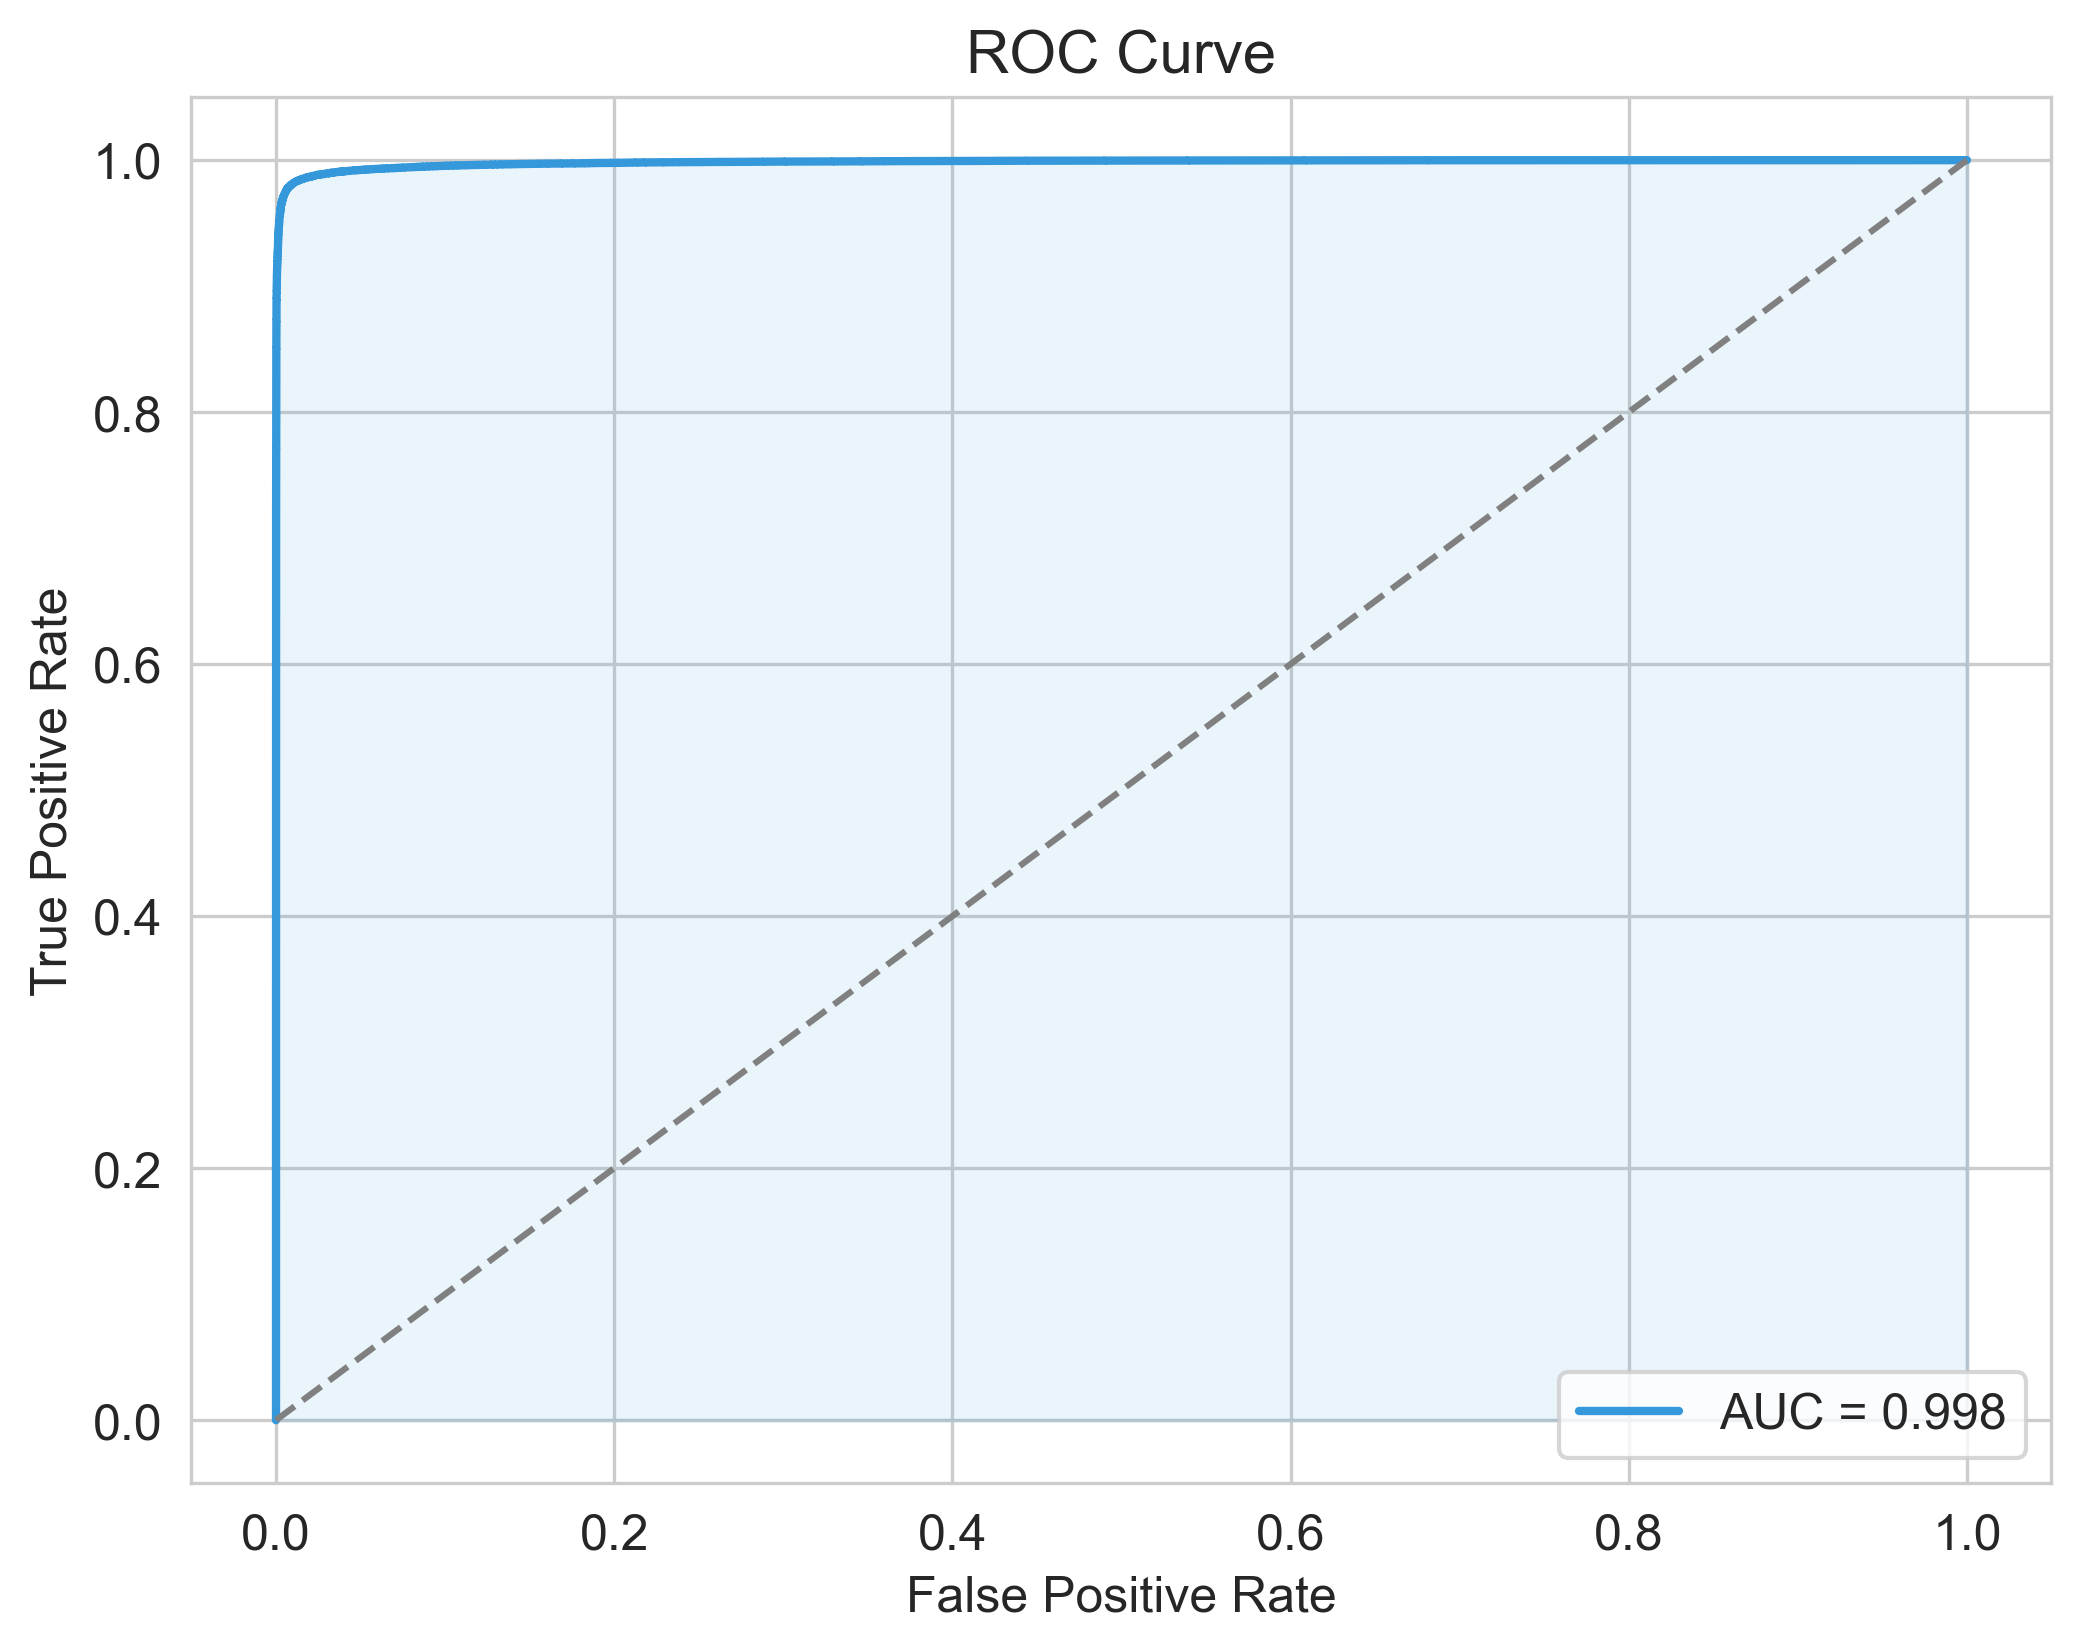
\includegraphics[width=0.8\textwidth]{../analysis/url/roc_curve.png}
    \caption{ROC Curve for URL Model}
    \label{fig:roc_curve_1}
\end{figure}

\begin{figure}[htbp]
    \centering
    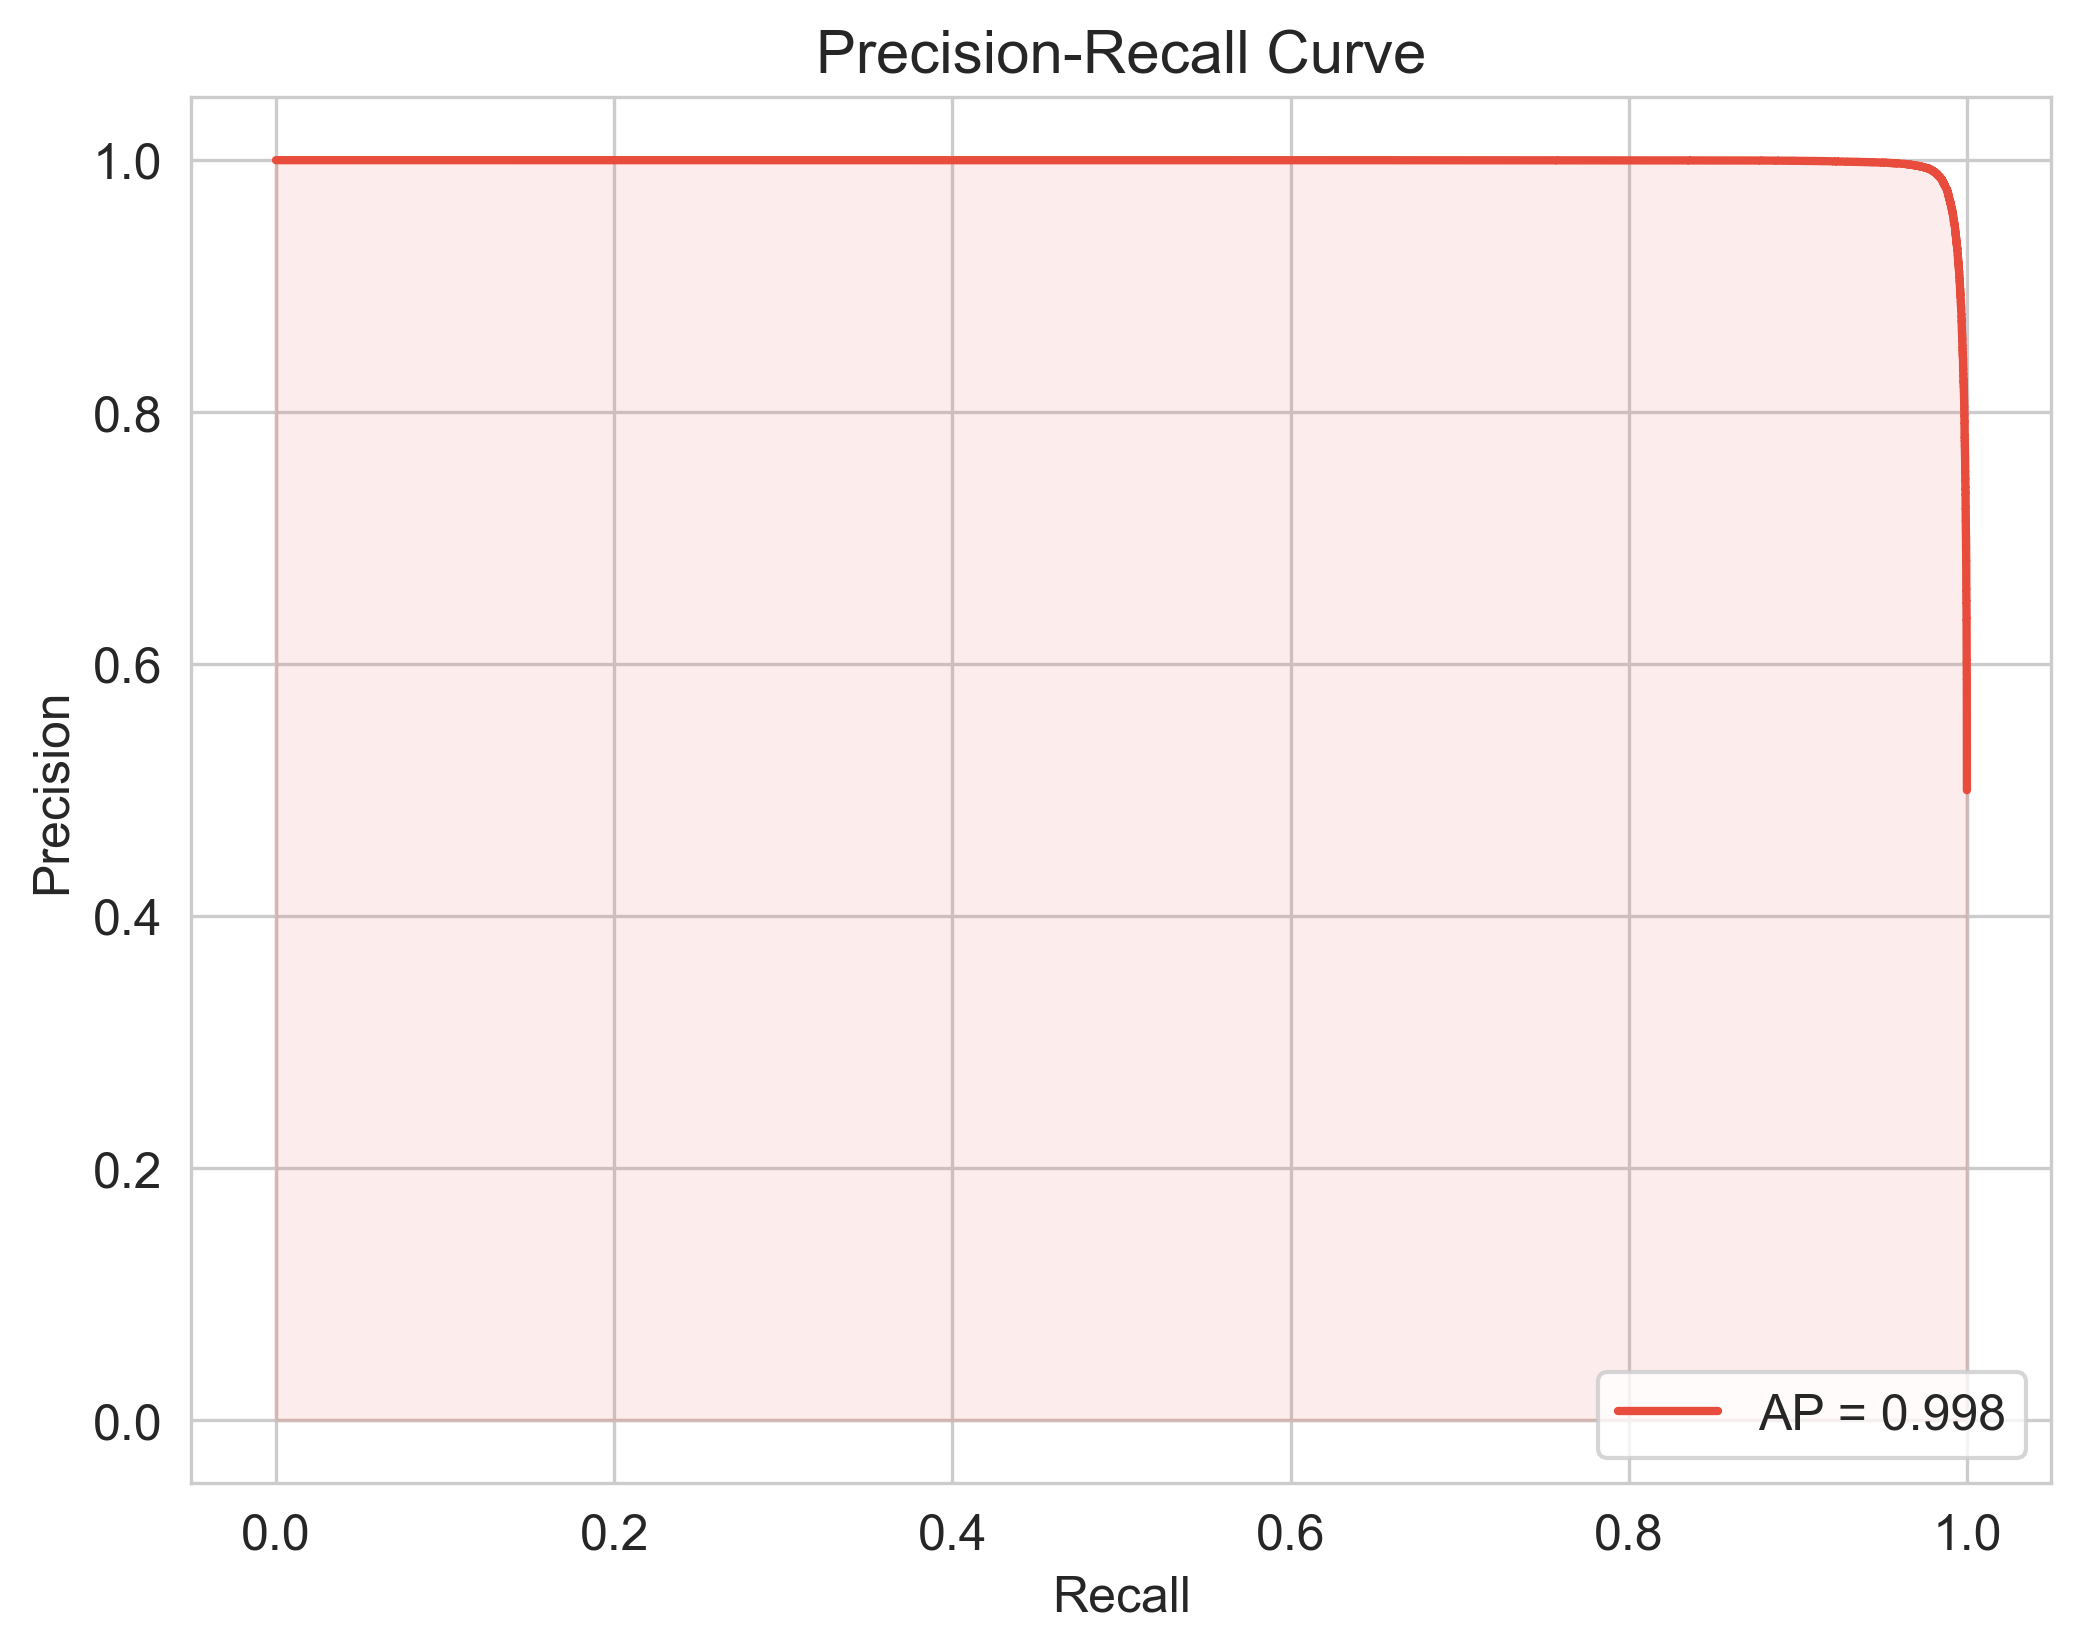
\includegraphics[width=0.8\textwidth]{../analysis/url/precision_recall_curve.png}
    \caption{Precision-Recall Curve for URL Model}
    \label{fig:precision_recall_curve_1}
\end{figure}

\begin{figure}[htbp]
    \centering
    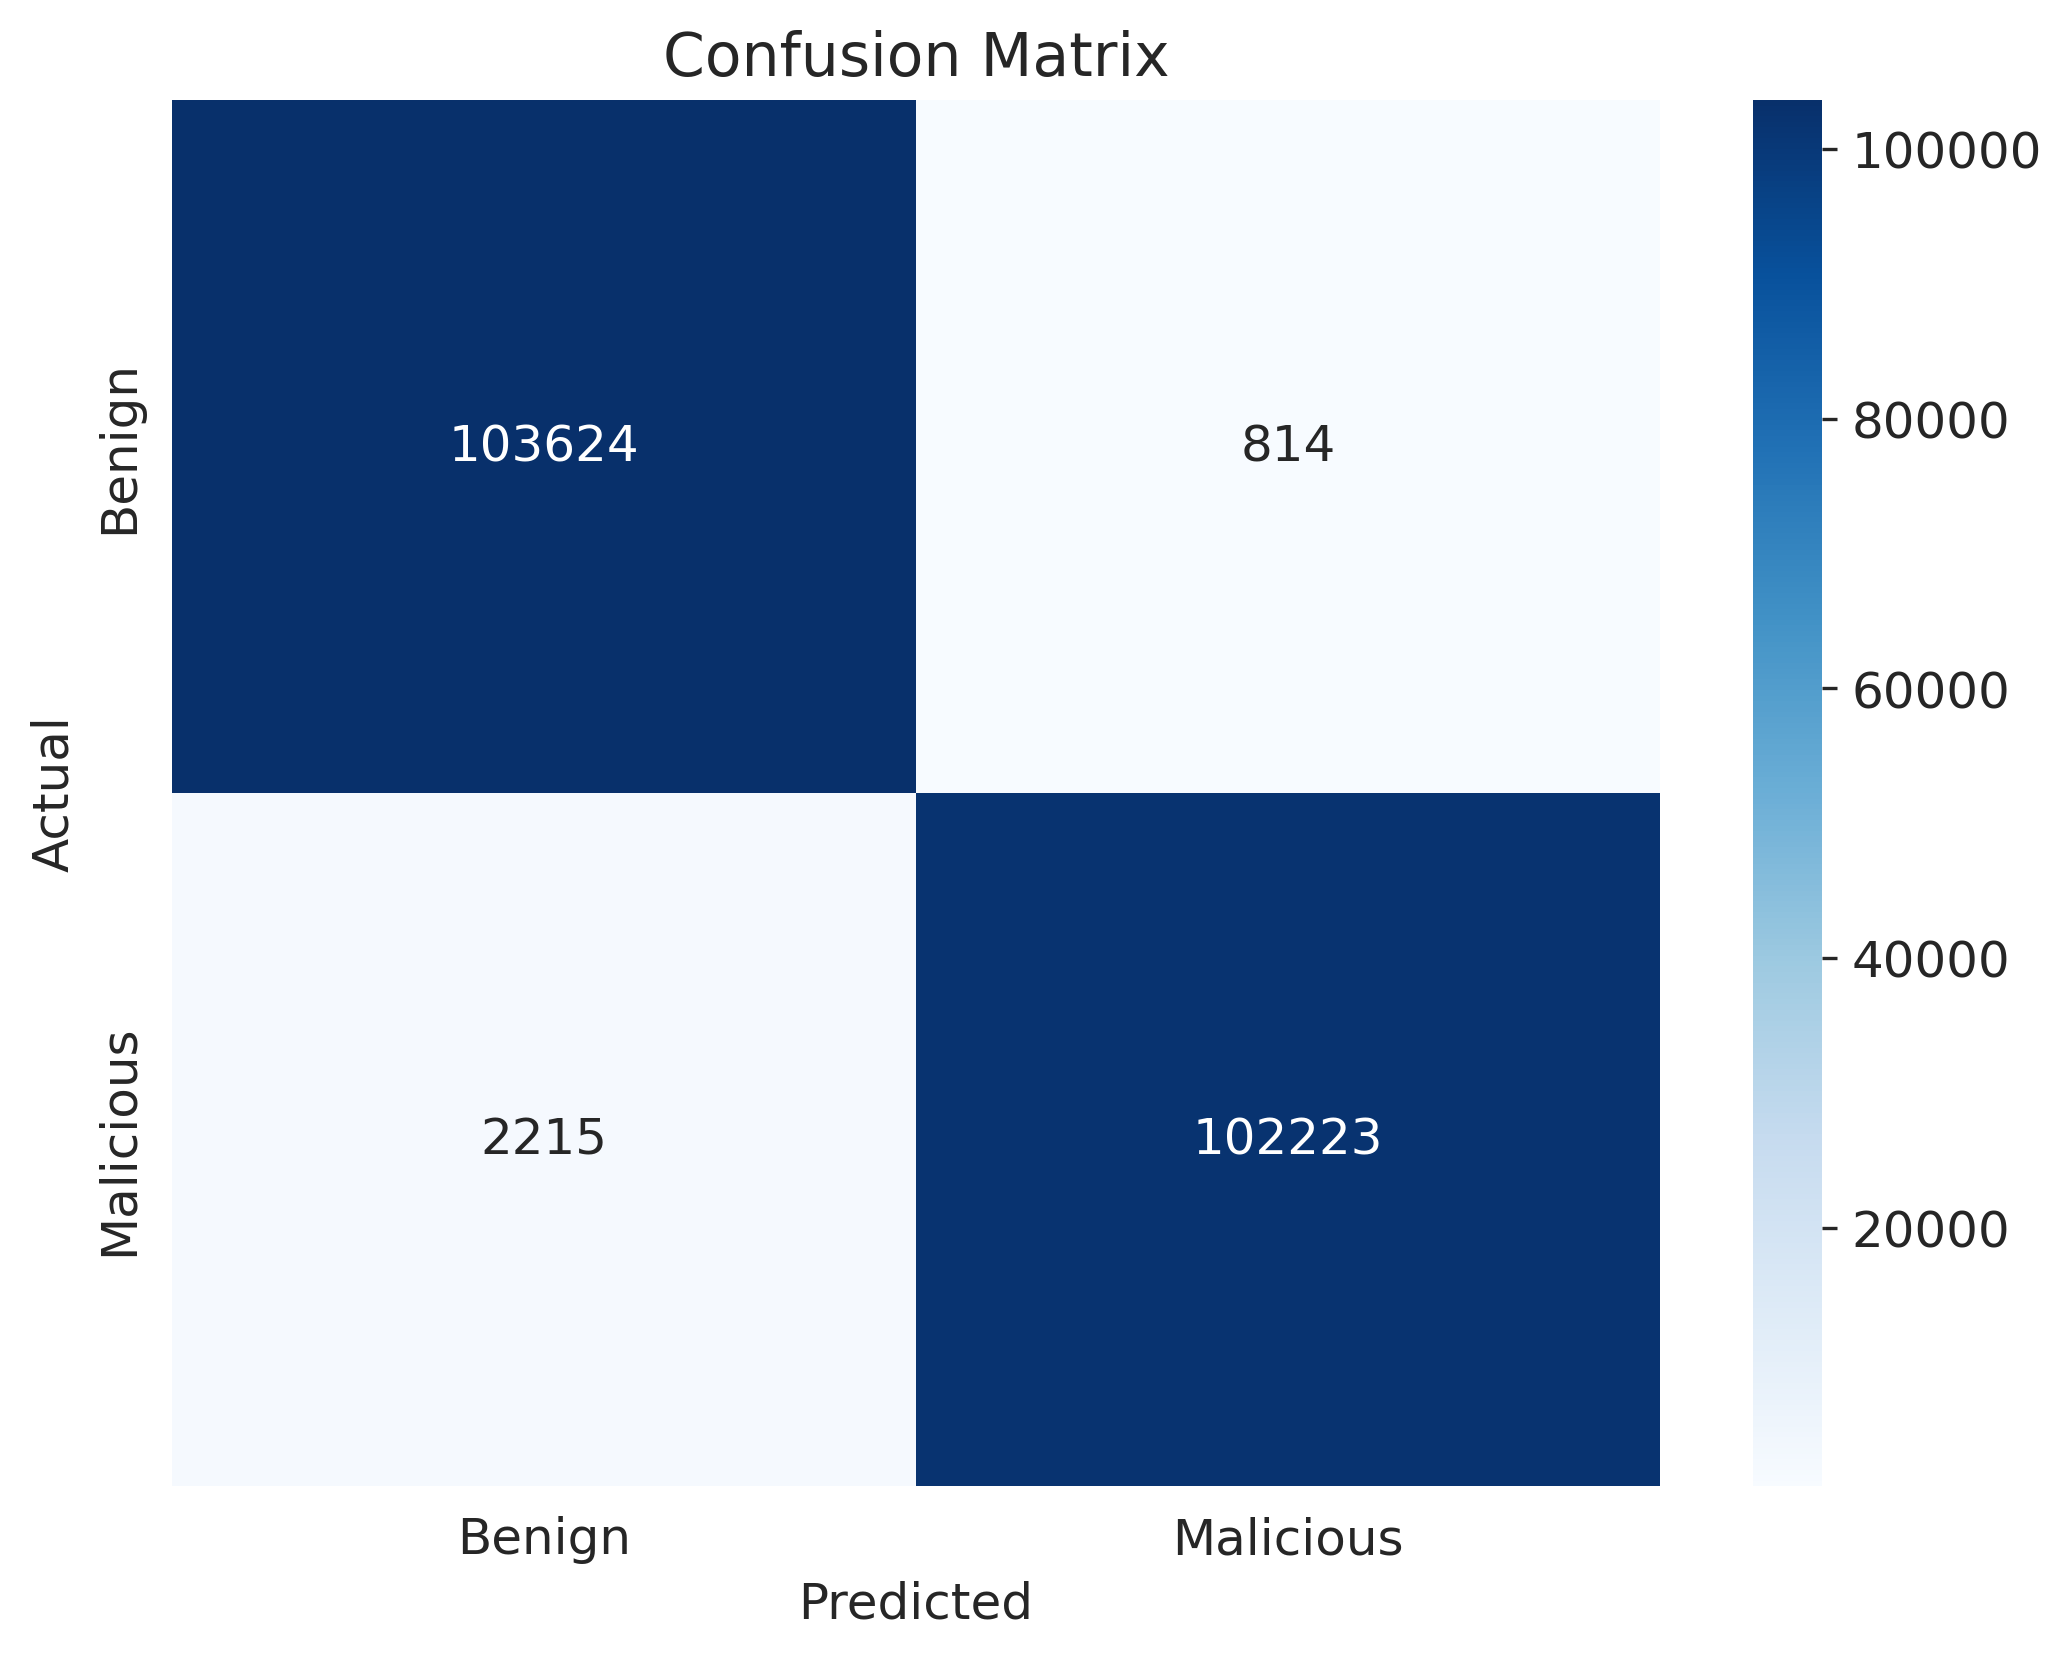
\includegraphics[width=0.8\textwidth]{../analysis/url/confusion_matrix.png}
    \caption{Confusion Matrix for URL Model}
    \label{fig:confusion_matrix_1}
\end{figure}

\subsubsection{SMS Model}
\subsubsection*{Feature Extraction}

We applied TF-IDF vectorization to capture word patterns and important terms while filtering out common English stopwords. The vectorization settings included:
\begin{itemize}
    \item Maximum features: 5000
    \item Minimum document frequency: 2
    \item Maximum document frequency: 0.95
\end{itemize}

\noindent
Training was done on the same laptop using \textbf{Stratified K-fold with 10 folds}. However, this time a \textbf{Random Forest Classifier} was used with the following hyperparameters:

\begin{itemize}
    \item 200 estimators
    \item Max depth of 30
\end{itemize}

\noindent
The model achieved the following results after training 6306 rows, taking around \textbf{54 secs}:

\begin{itemize}
    \item Accuracy: \textbf{96.73\%}
    \item AUC: \textbf{99.16\%}
    \item Average Precision: \textbf{99.34\%}
\end{itemize}

\begin{table}[htbp]
    \centering
    \caption{\textbf{SMS model Classification Report}}
    \begin{tabular}{l c c c c}
    \toprule
     & \textbf{Precision} & \textbf{Recall} & \textbf{F1-Score} & Support \\
    \midrule
    \textbf{Ham} & \textbf{0.96} & \textbf{0.97} & \textbf{0.97} & 3153 \\
    \textbf{Spam} & \textbf{0.97} & \textbf{0.96} & \textbf{0.97} & 3153 \\
    \midrule
    \textbf{Accuracy} & & & \textbf{0.97} & 6306 \\
    Macro Avg & 0.97 & 0.97 & 0.97 & 6306 \\
    Weighted Avg & 0.97 & 0.97 & 0.97 & 6306 \\
    \bottomrule
    \end{tabular}
    \label{tab:classification_report_2}
\end{table}

\noindent
Additionally, the following ROC curve, Precision-Recall curve, and confusion matrix were generated to visualize the model's performance:

\begin{figure}[htbp]
    \centering
    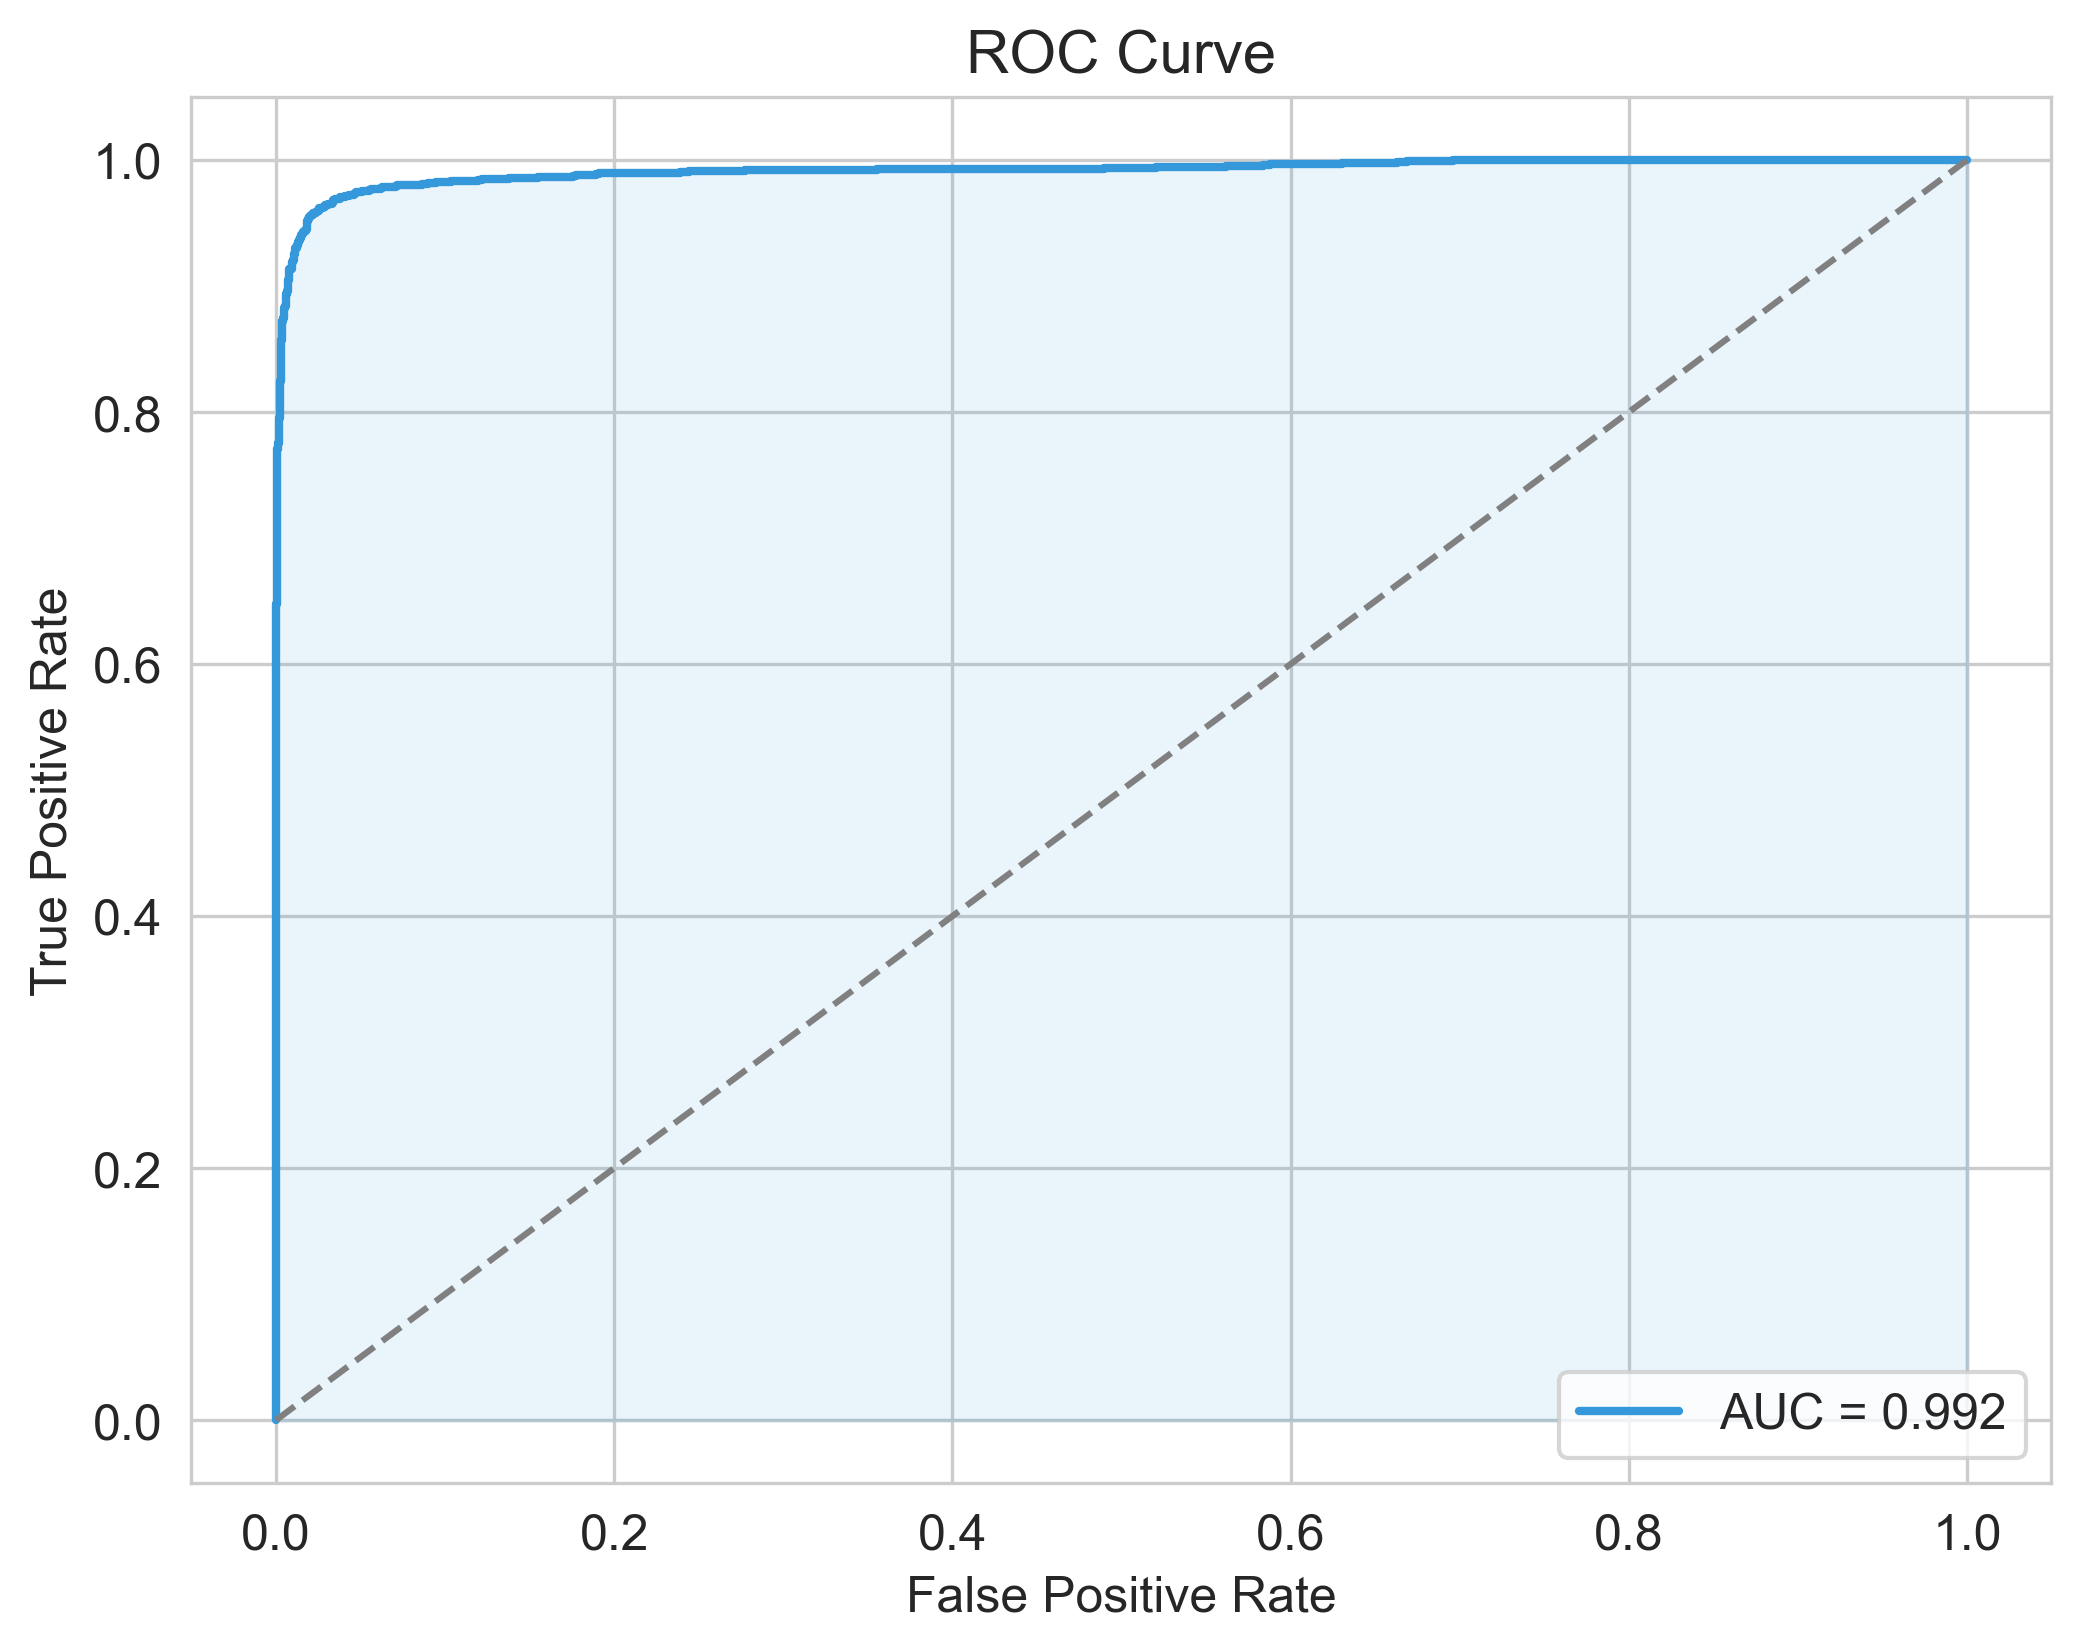
\includegraphics[width=0.8\textwidth]{../analysis/sms/randomforest/roc_curve.png}
    \caption{ROC Curve for SMS Model}
    \label{fig:roc_curve_2}
\end{figure}

\begin{figure}[htbp]
    \centering
    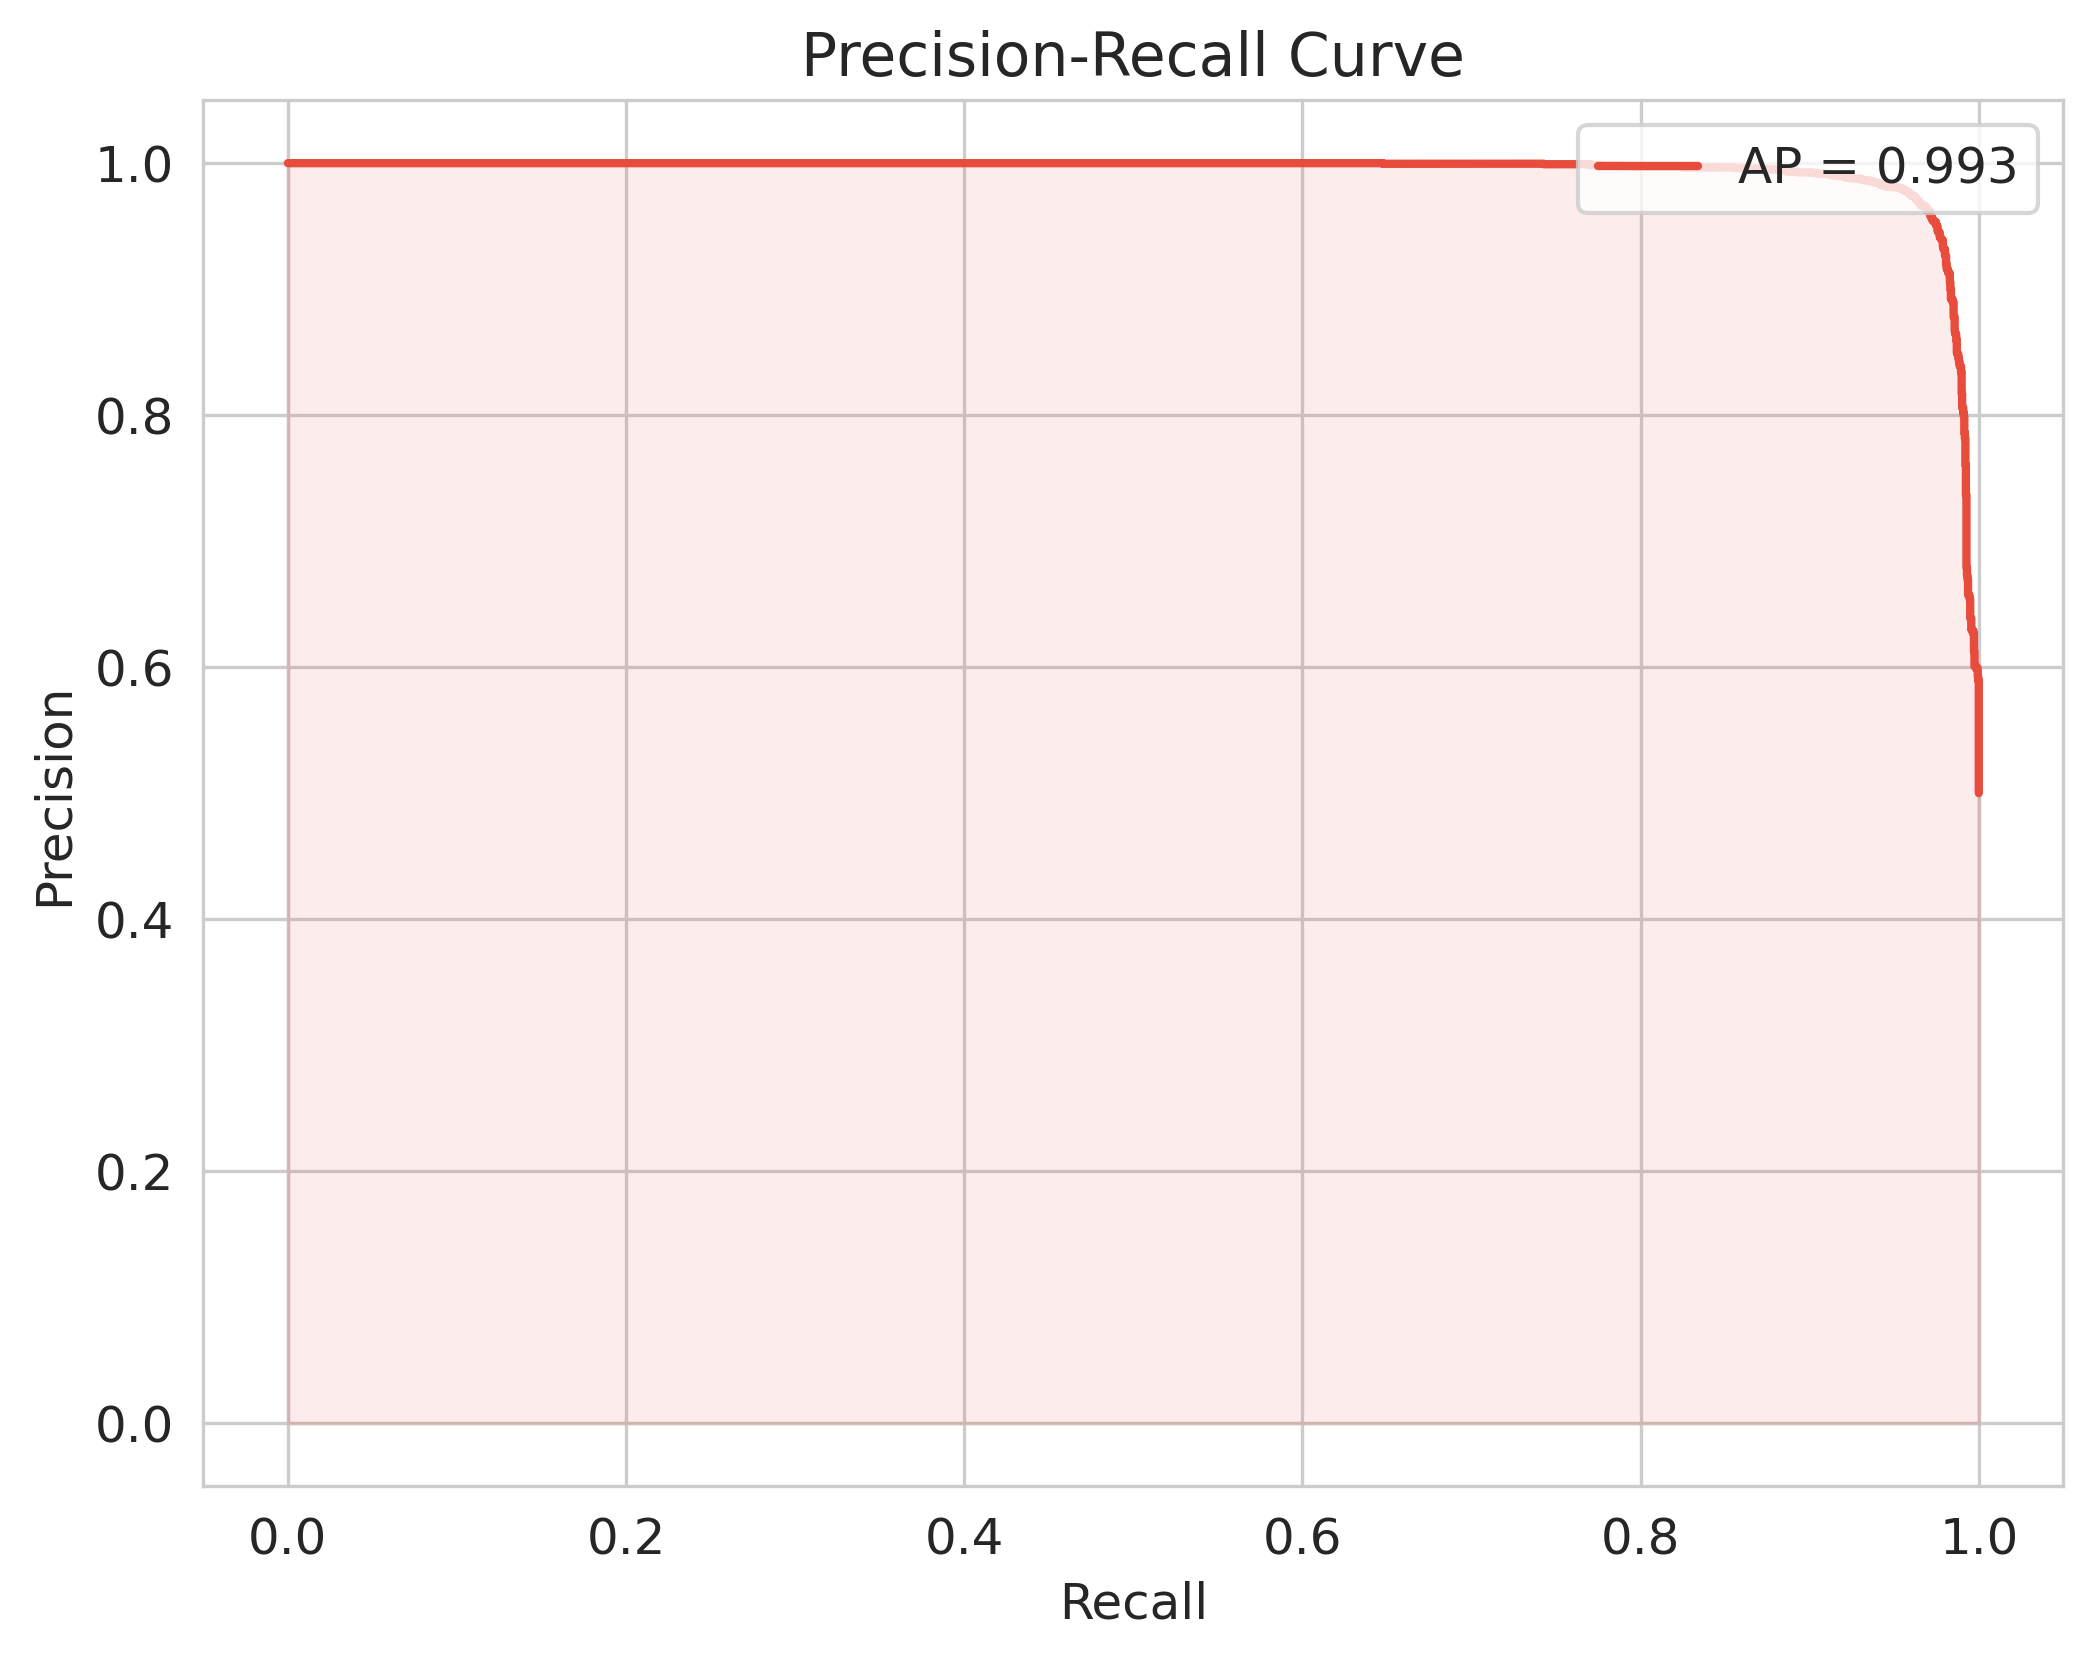
\includegraphics[width=0.8\textwidth]{../analysis/sms/randomforest/precision_recall_curve.png}
    \caption{Precision-Recall Curve for SMS Model}
    \label{fig:precision_recall_curve_2}
\end{figure}

\begin{figure}[htbp]
    \centering
    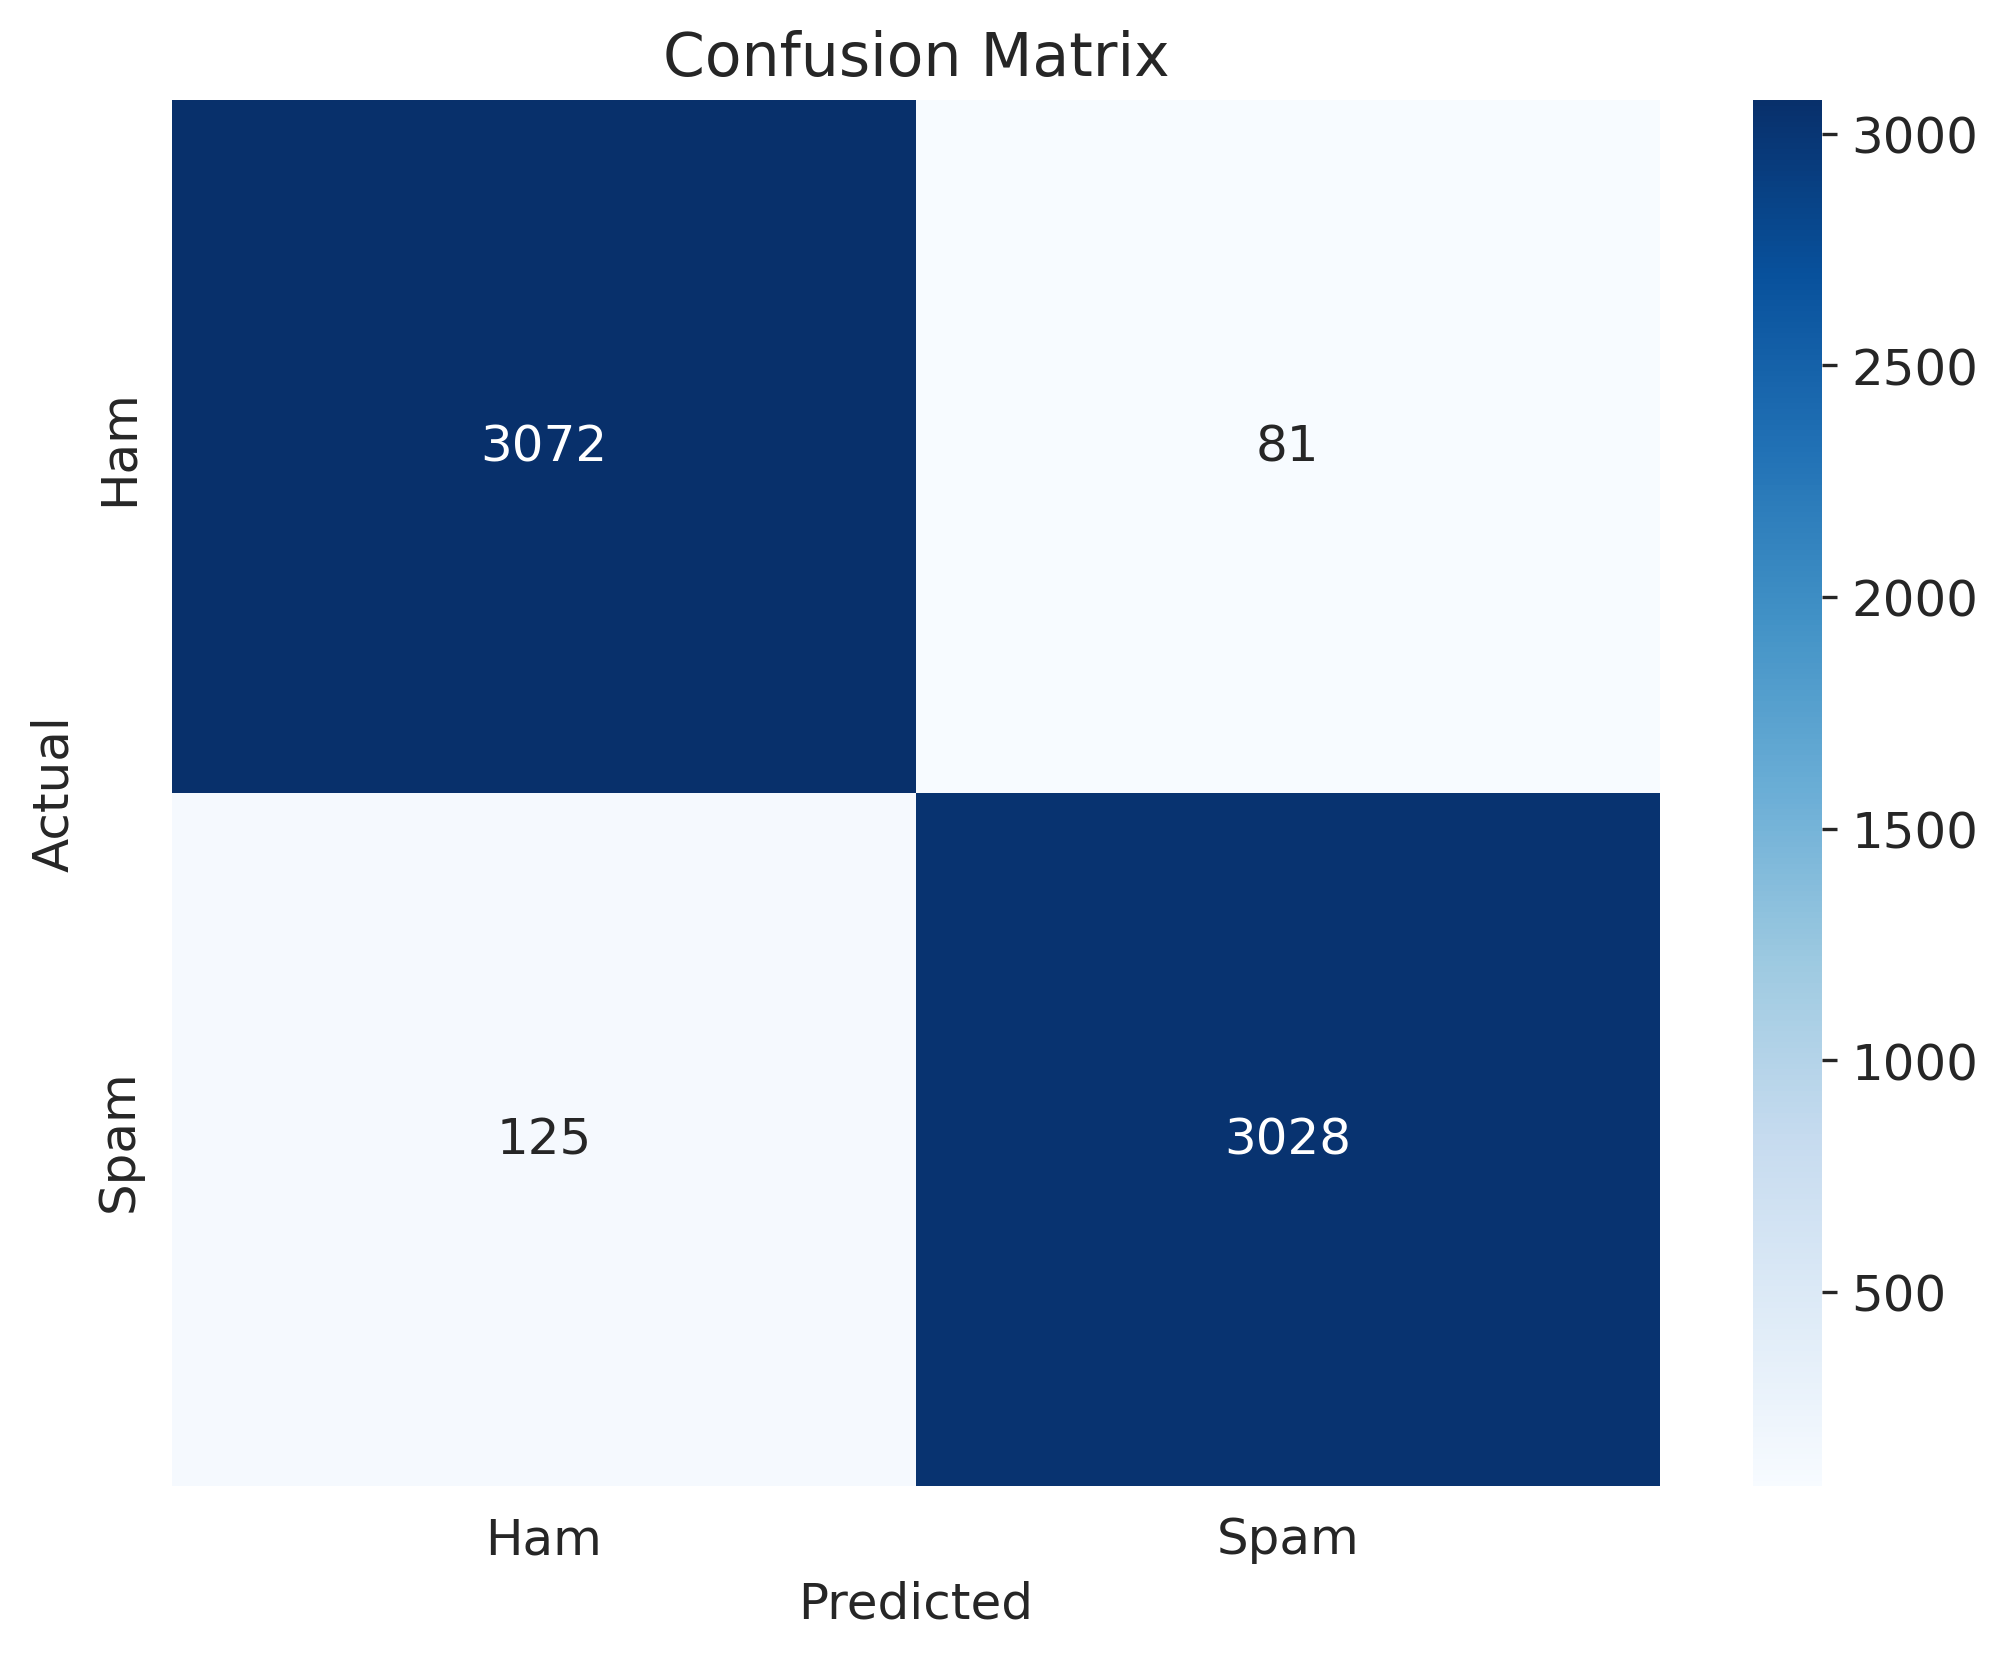
\includegraphics[width=0.8\textwidth]{../analysis/sms/randomforest/confusion_matrix.png}
    \caption{Confusion Matrix for SMS Model}
    \label{fig:confusion_matrix_2}
\end{figure}

\newpage

\noindent
    Furthermore, when training the model, we also decided to use another approach where we only train using the \textbf{SMS UCI Spam Collection Dataset} [2], using the same normalization approach (Balancing spam and non spam values, removing whitespaces, urls, etc). This was done to compare our results with the results of the study by Gawai and Salunke [8]. The model achieved the following results after training \textbf{1494 rows} (Much smaller than original SMS UCI dataset as there is a heavy bias), taking around \textbf{17 secs}: 

\begin{itemize}
    \item Accuracy: \textbf{97.19\%}
    \item AUC: \textbf{99.34\%}
    \item Average Precision: \textbf{99.48\%}
\end{itemize}

\begin{table}[htbp]
    \centering
    \caption{\textbf{SMS model Classification Report}}
    \begin{tabular}{l c c c c}
    \toprule
     & \textbf{Precision} & \textbf{Recall} & \textbf{F1-Score} & Support \\
    \midrule
    \textbf{Legitimate} & \textbf{0.96} & \textbf{0.99} & \textbf{0.97} & 747 \\
    \textbf{Spam} & \textbf{0.99} & \textbf{0.96} & \textbf{0.97} & 747 \\
    \midrule
    \textbf{Accuracy} & & & \textbf{0.97} & 1494 \\
    Macro Avg & 0.97 & 0.97 & 0.97 & 1494 \\
    Weighted Avg & 0.97 & 0.97 & 0.97 & 1494 \\
    \bottomrule
    \end{tabular}
    \label{tab:classification_report_3}
\end{table}

\noindent
We also generated the following ROC curve, Precision-Recall curve, and confusion matrix to visualize the model's performance:

\begin{figure}[htbp]
    \centering
    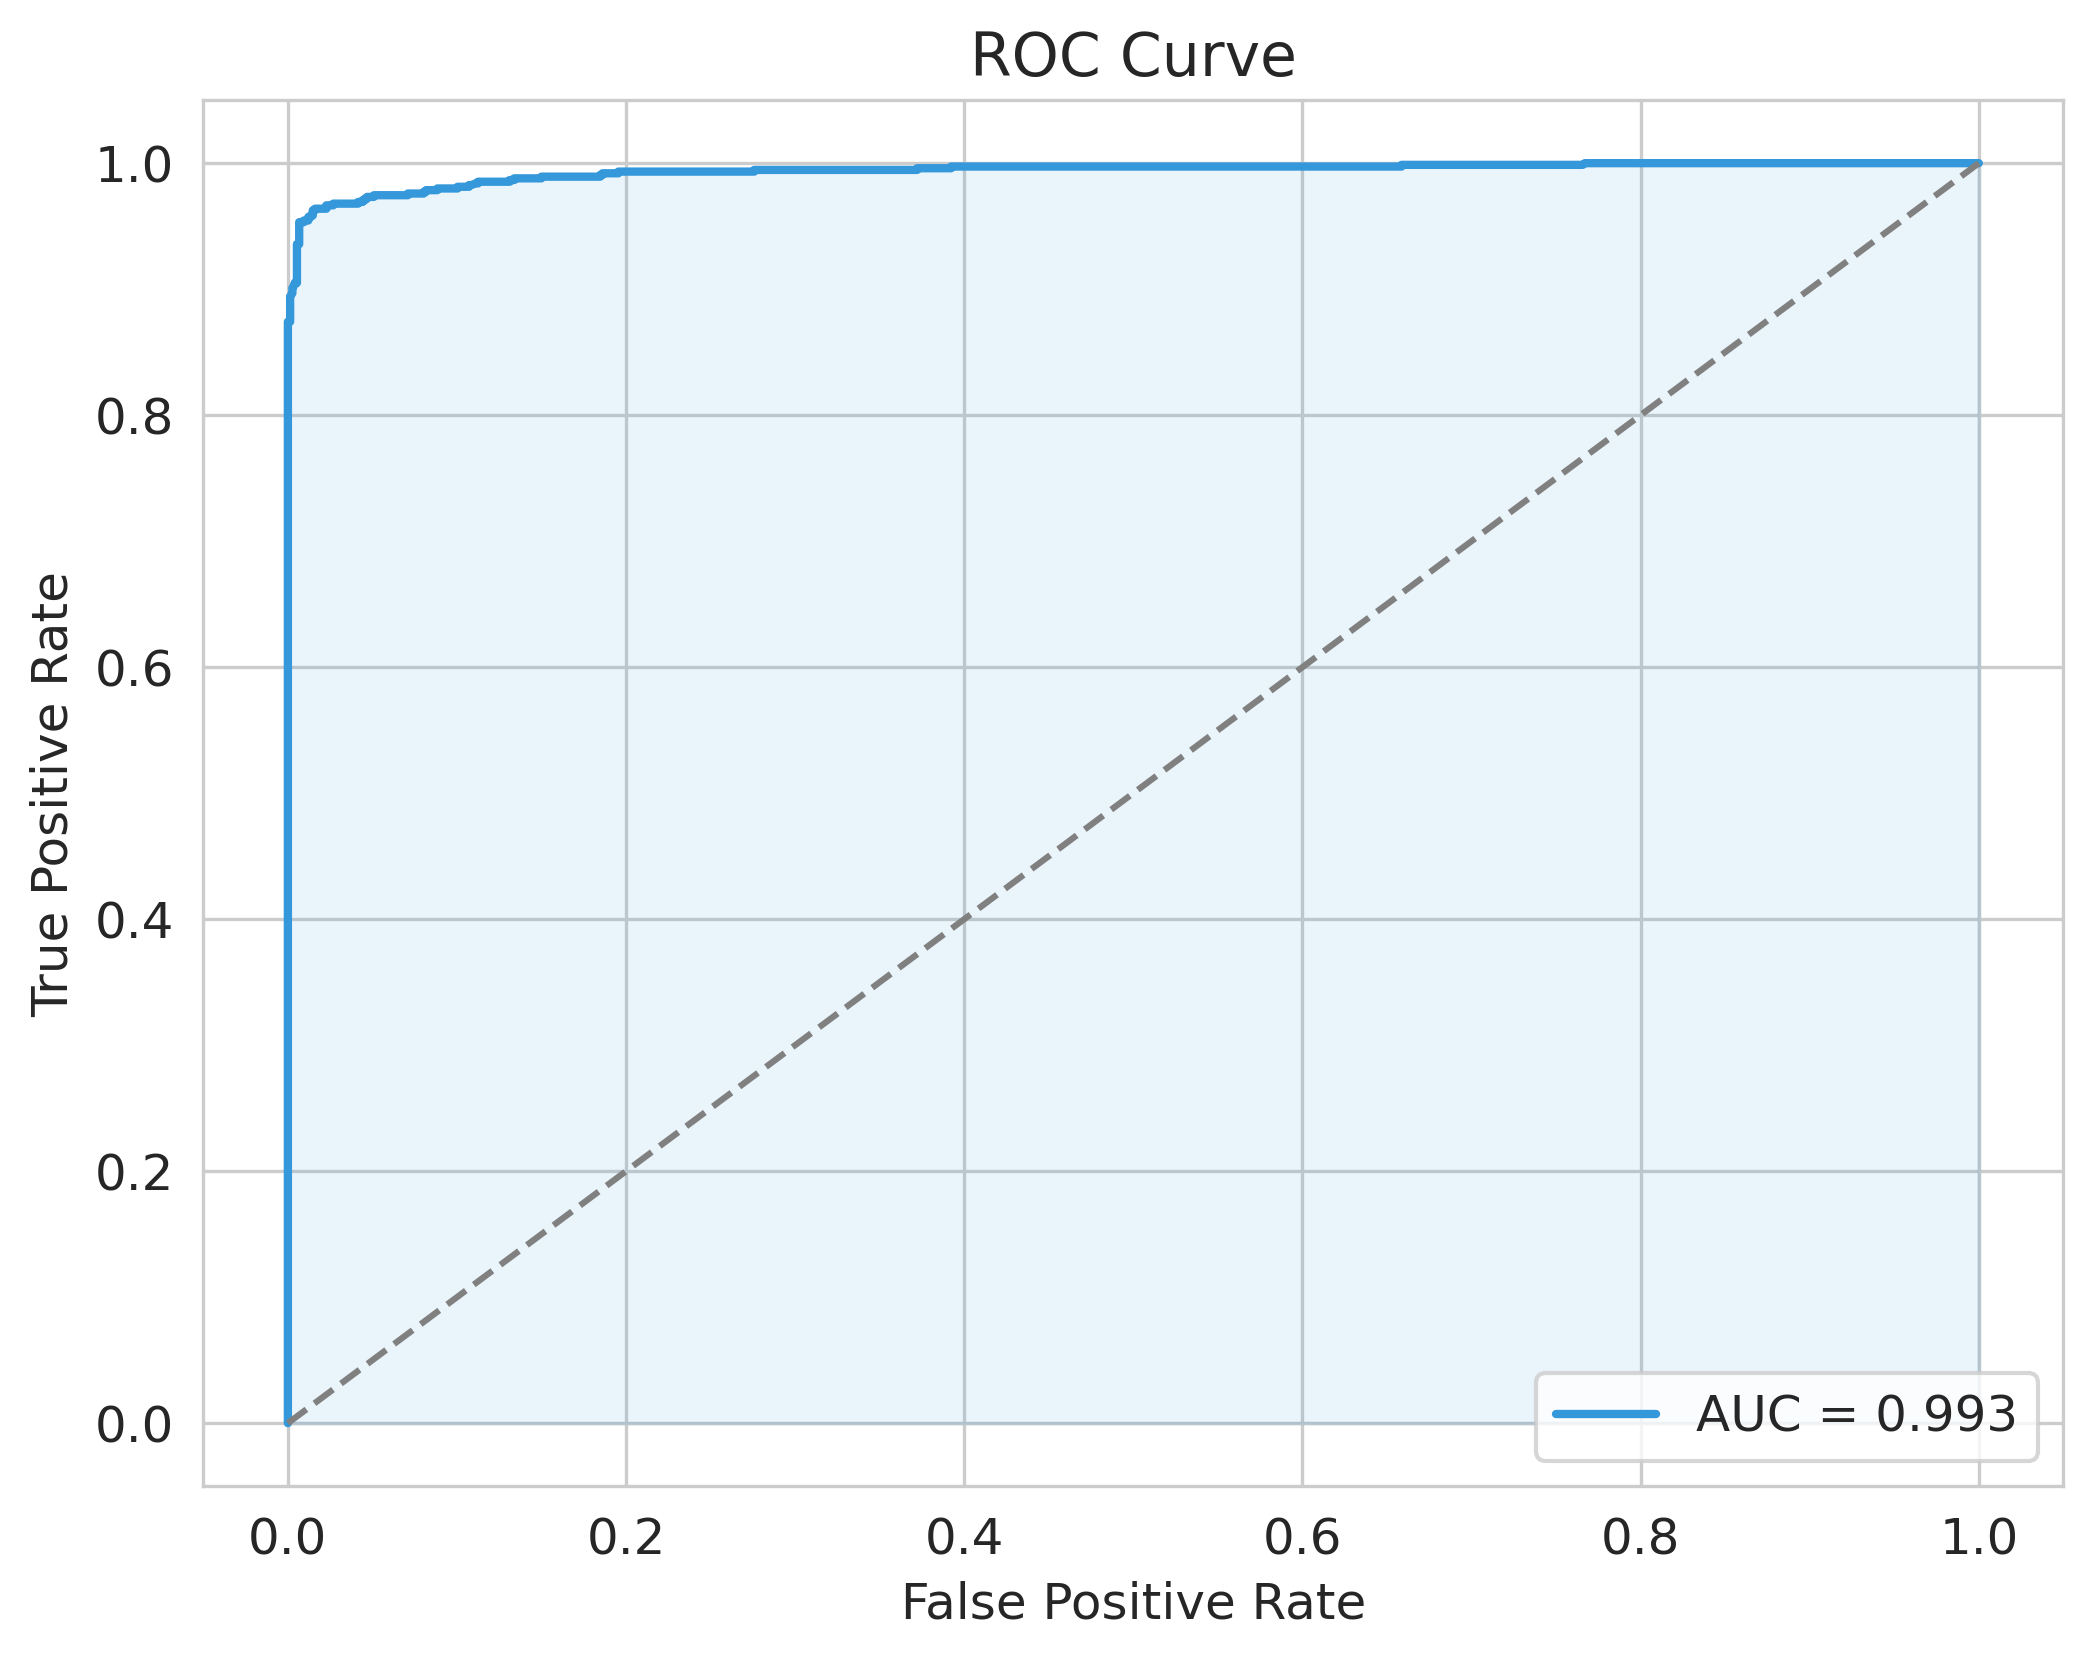
\includegraphics[width=0.8\textwidth]{../analysis/sms/randomforest/uci/roc_curve.png}
    \caption{ROC Curve for SMS Model (UCI Dataset)}
    \label{fig:roc_curve_3}
\end{figure}

\begin{figure}[htbp]
    \centering
    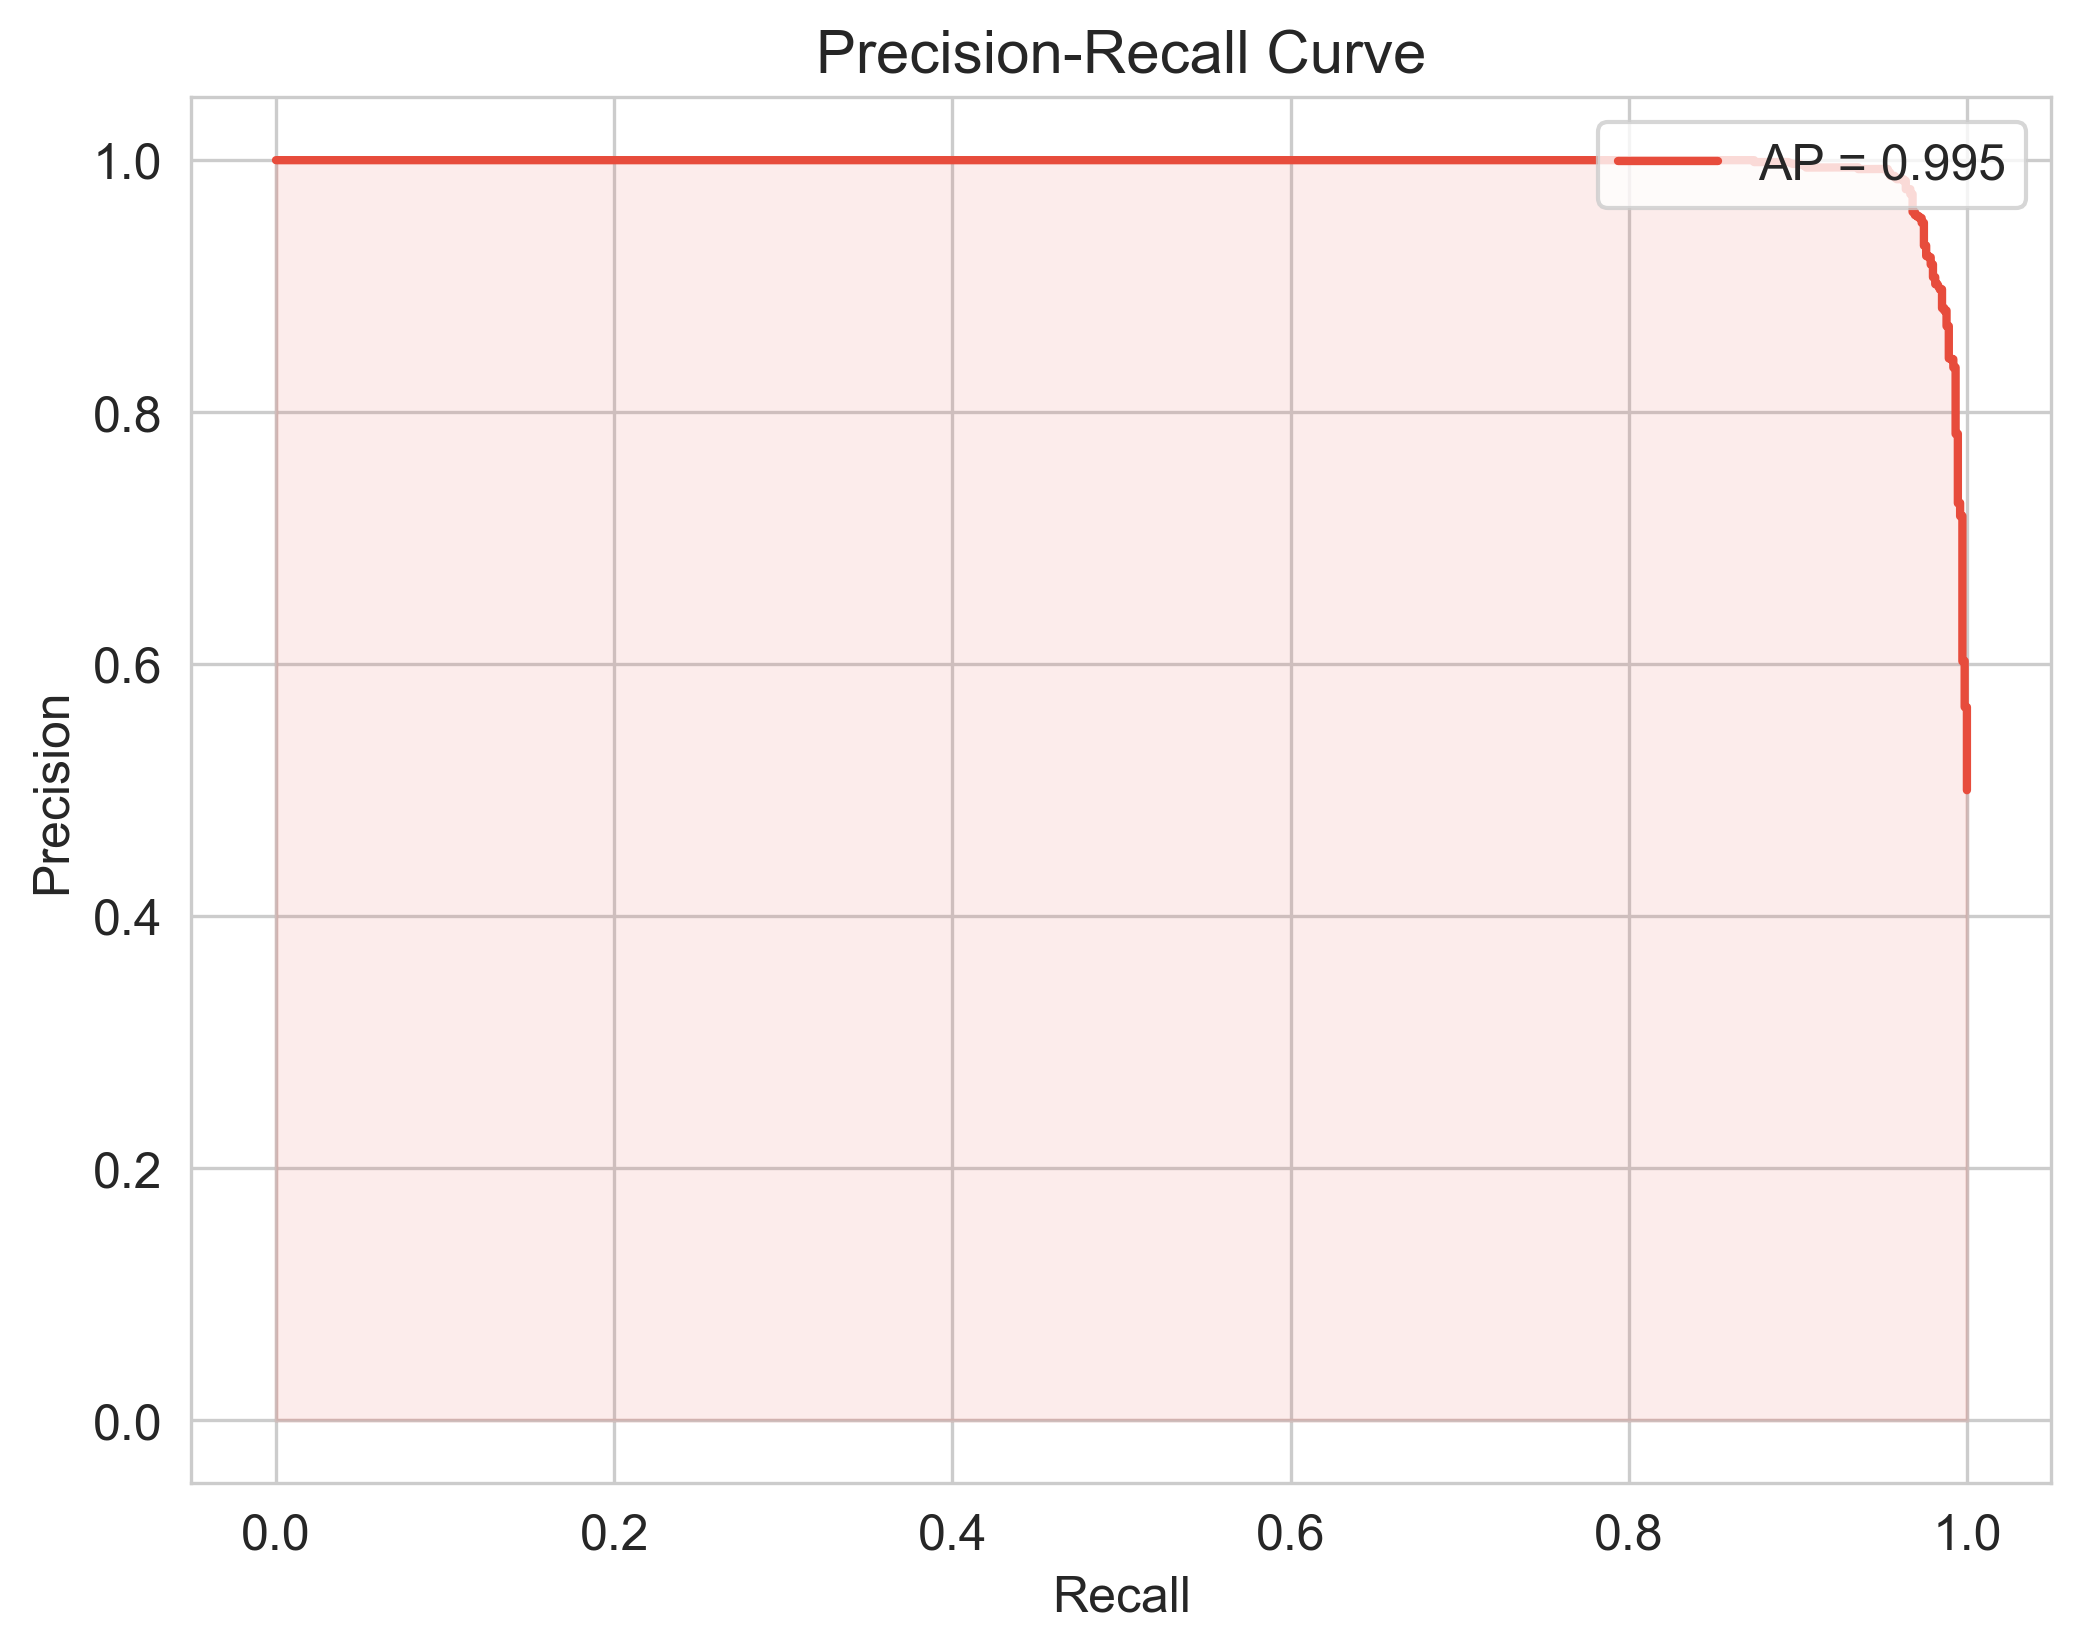
\includegraphics[width=0.8\textwidth]{../analysis/sms/randomforest/uci/precision_recall_curve.png}
    \caption{Precision-Recall Curve for SMS Model (UCI Dataset)}
    \label{fig:precision_recall_curve_3}
\end{figure}

\begin{figure}[htbp]
    \centering
    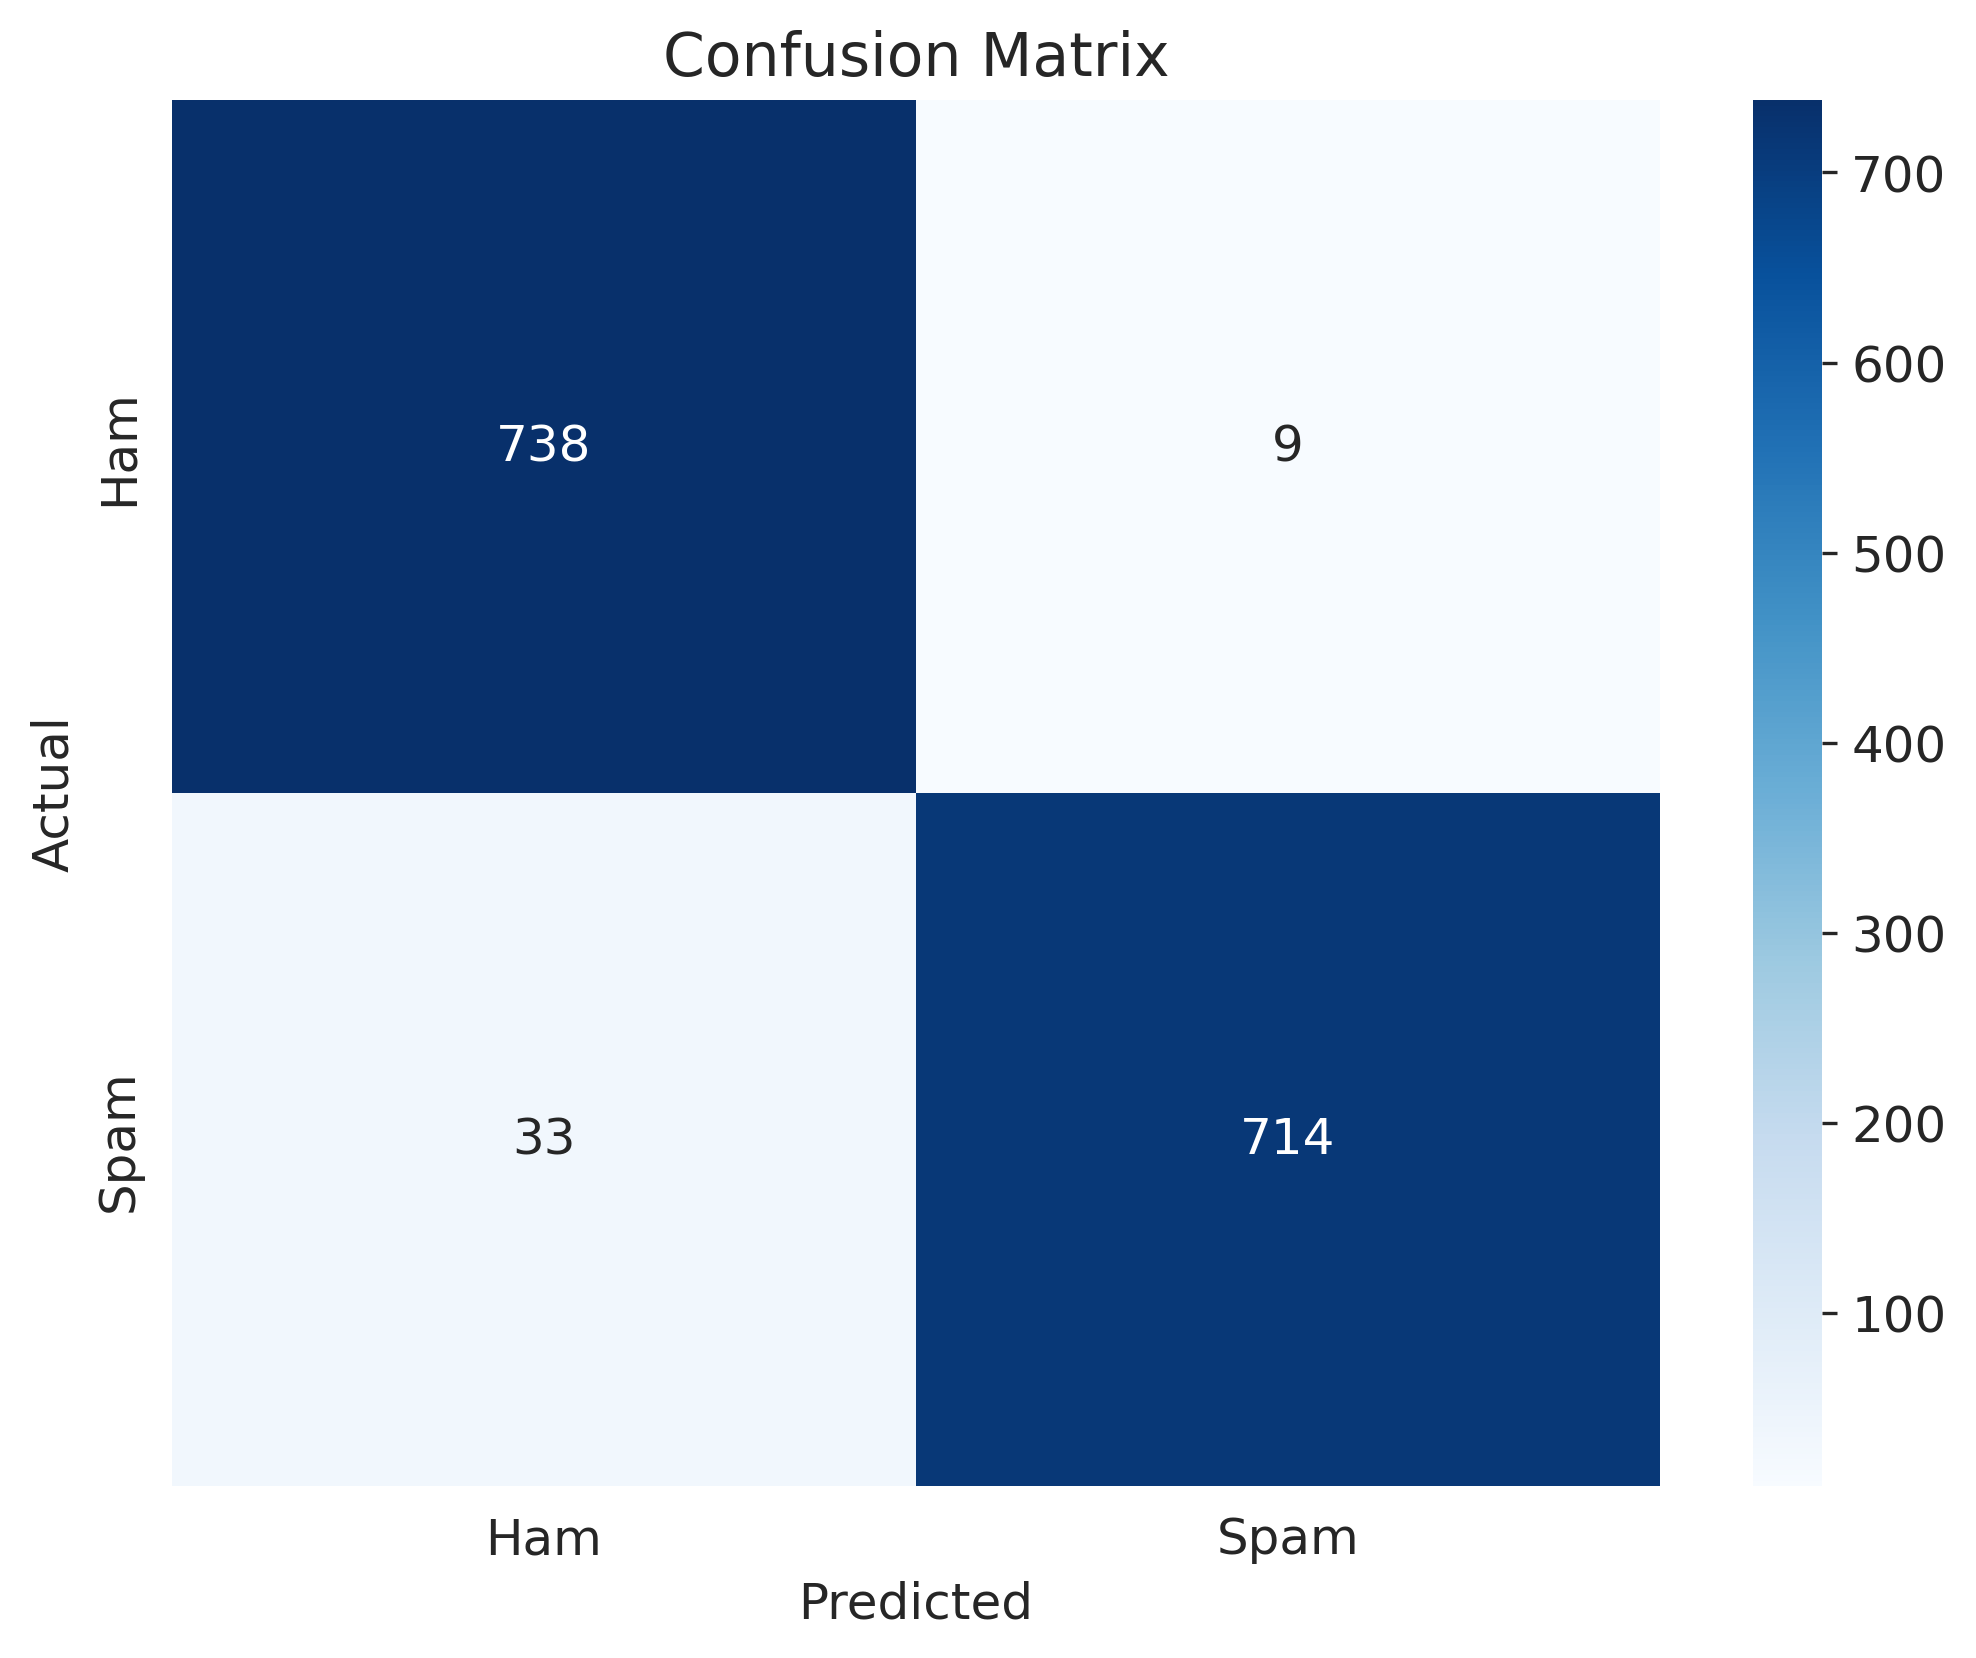
\includegraphics[width=0.8\textwidth]{../analysis/sms/randomforest/uci/confusion_matrix.png}
    \caption{Confusion Matrix for SMS Model (UCI Dataset)}
    \label{fig:confusion_matrix_3}
\end{figure}

\newpage

\subsubsection{Email Model}
\subsubsection*{Feature Extraction}
We applied TF-IDF vectorization separately to both the email subject and body, allowing the model to leverage textual patterns in each section.
\newline
\newline
Text vectorization settings:
\begin{itemize}
    \item Minimum document frequency: 3
    \item Maximum document frequency: 0.90
    \item 5000 max features
\end{itemize}

\noindent
Subject vectorization settings:
\begin{itemize}
    \item Minimum document frequency: 2
    \item Maximum document frequency: 0.95
    \item 1000 max features
\end{itemize}

\subsubsection*{Training}
We trained an \textbf{XGBoost classifier} (No Stratified K-fold), with the same hardware but with a \textbf{70/30 train-test split}:

\begin{itemize}
    \item 500 estimators
    \item Max depth of 10
    \item Learning rate of 0.05
    \item Subsampling of 0.8
    \item Early stopping at 30 rounds if no improvement
\end{itemize}

\noindent
The model achieved the following results after training 23000 rows, taking 249 secs:

\begin{itemize}
    \item Accuracy: \textbf{96.90\%}
    \item AUC: \textbf{99.59\%}
    \item Average Precision: \textbf{99.55\%}
\end{itemize}

\begin{table}[htbp]
    \centering
    \caption{Email Model Evaluation Report}
    \begin{tabular}{l c c c c}
    \toprule
     & \textbf{Precision} & \textbf{Recall} & \textbf{F1-Score} & Support \\
    \midrule
    \textbf{Legitimate} & \textbf{0.99} & \textbf{0.95} & \textbf{0.97} & 2649 \\
    \textbf{Spam} & \textbf{0.95} & \textbf{0.99} & \textbf{0.97} & 2649 \\
    \midrule
    \textbf{Accuracy}  & & & \textbf{0.97} & 5297 \\
    Macro Avg & 0.97 & 0.97 & 0.97 & 5297 \\
    Weighted Avg & 0.97 & 0.97 & 0.97 & 5297 \\
    \bottomrule
    \end{tabular}
    \label{tab:xgboost_evaluation}
\end{table}


\subsubsection{YouTube Comments Model}
\subsubsection*{Feature Extraction}

Here, we once again utilize a TF-IDF vectorizer for text, as well as one for author.

\begin{itemize}
    \item Textual Features: TF-IDF vectorization applied to comment text
    \item Author Based Features: TF-IDF vectorization applied to usernames to detect repeated spam patterns from specific users, as well as recognize patterns in usernames that look suspicious
\end{itemize}

\subsubsection*{Training}

Here, we train using a \textbf{Gradient Boosting Classifier} mainly so we can capture hierarchical relationships within the text data, since they are comments. This is all done using the same hardware and with a 70/30 train-test split. The hyperparameters include:

\begin{itemize}
    \item 200 estimators
    \item Max depth of 6
    \item Learning rate of 0.05
    \item Subsampling of 0.7
\end{itemize}

\noindent
The model achieved the following results after training 1962 rows, taking 0.73 secs:

\begin{itemize}
    \item Accuracy: \textbf{94.22\%}
    \item AUC: \textbf{98.65\%}
    \item Average Precision: \textbf{98.78\%}
\end{itemize}

\begin{table}[htbp]
    \centering
    \caption{YouTube Comments Model Evaluation Report}
    \begin{tabular}{l c c c c}
    \toprule
     & \textbf{Precision} & \textbf{Recall} & \textbf{F1-Score} & Support \\
    \midrule
    \textbf{Legitimate} & \textbf{0.91} & \textbf{0.98} & \textbf{0.94} & 286 \\
    \textbf{Spam} & \textbf{0.98} & \textbf{0.91} & \textbf{0.94} & 285 \\
    \midrule
    \textbf{Accuracy}  & & & \textbf{0.94} & 571 \\
    Macro Avg & 0.94 & 0.94 & 0.94 & 571 \\
    Weighted Avg & 0.94 & 0.94 & 0.94 & 571 \\
    \bottomrule
    \end{tabular}
    \label{tab:gbm_evaluation}
\end{table}

\newpage

\section{Inference}

The inference process across SMS, email, and comments, generally follows the same execution steps While the specifics vary slightly for each type of message, the overall approach remains the same.


\subsection{Preprocessing and Feature Extraction}

\begin{enumerate}
    \item URL Cleaning: Any URLs present in the text are extracted and normalized.
    \item Vectorization: The cleaned text is transformed using pre-trained vectorizers specific to each message type (SMS, email, comments). Email subjects and comment author names are also vectorized where applicable.
    \item URL Feature Extraction: If URLs are found in the text, a feature extraction function analyzes them based on characteristics such as length, presence of suspicious keywords, and domain reputation, as done within the training scripts feature extractor.
\end{enumerate}

\subsection{Probability Estimation}

\begin{enumerate}
    \item Text Classification: The vectorized text is passed through a trained classification model that returns a spam probability score.
    \item URL Spam Detection: If URLs are present, they are sent into the URL model to predict the likelihood of them being malicious or spam-related.
    \item Weighted Combination: The probability scores from text classification and URL analysis are combined using a weighted sum approach. The weight distribution varies depending on the message type, with URL spam probability often given higher significance if URLs are detected.
\end{enumerate}

\subsection{Final Decision}

The final spam probability score is then compared against a predefined threshold (typically 0.5). If the score meets or exceeds this threshold, the message is classified as spam; otherwise, it is classified as non-spam.

\section{Results and Discussion}
\subsection{Comparison to Traditional Methods}

\noindent
As mentioned previously, the study by Gawai and Salunke [8] aimed to compare the performance of various machine learning algorithms for SMS spam detection. The results of their study are shown within the table below:

\begin{table}[htbp]
    \centering
    \caption{Performance of different algorithms by Gawai and Salunke [8]} % Replace with your desired caption
    \label{tab:performance} % Add a label for referencing
    
    \begin{tabular}{l cccc cccc c}
    \toprule
    \textbf{Algorithms} & \multicolumn{2}{c}{\textbf{Precision}} & \multicolumn{2}{c}{\textbf{Recall}} & \multicolumn{2}{c}{\textbf{F1-Score}} & \textbf{Accuracy} \\
    \cmidrule(lr){2-3} \cmidrule(lr){4-5} \cmidrule(lr){6-7}
    & Ham & Spam & Ham & Spam & Ham & Spam & \\
    \midrule
    SVM & 0.96 & 0.99 & 0.99 & 0.70 & 0.98 & 0.82 & 0.97 \\
    Decision Trees & 0.98 & 0.91 & 0.99 & 0.81 & 0.98 & 0.86 & 0.96 \\
    \textbf{Random Forest} & \textbf{0.97} & \textbf{0.99} & \textbf{0.99} & \textbf{0.79} & \textbf{0.99} & \textbf{0.88} & \textbf{0.97} \\
    KNN & 0.94 & 0.99 & 0.99 & 0.54 & 0.97 & 0.70 & 0.95 \\
    \textbf{Naïve Bayes} & \textbf{0.98} & \textbf{0.99} & \textbf{0.99} & \textbf{0.85} & \textbf{0.99} & \textbf{0.92} & \textbf{0.98} \\
    \bottomrule
    \end{tabular}
\end{table}

\newpage

\noindent
When utilizing the same dataset and training algorithms, we get the following results:

\begin{table}[htbp]
    \centering
    \caption{Performance of different algorithms, Our Results} % Replace with your desired caption
    \label{tab:performance} % Add a label for referencing
    
    \begin{tabular}{l cccc cccc c}
    \toprule
    \textbf{Algorithms} & \multicolumn{2}{c}{\textbf{Precision}} & \multicolumn{2}{c}{\textbf{Recall}} & \multicolumn{2}{c}{\textbf{F1-Score}} & \textbf{Accuracy} \\
    \cmidrule(lr){2-3} \cmidrule(lr){4-5} \cmidrule(lr){6-7}
    & Ham & Spam & Ham & Spam & Ham & Spam & \\
    \midrule
    SVM & 0.96 & 0.99 & 0.99 & 0.96 & 0.97 & 0.97 & 0.97 \\
    Decision Trees & 0.94 & 0.94 & 0.94 & 0.94 & 0.94 & 0.94 & 0.96 \\
    \textbf{Random Forest} & \textbf{0.96} & \textbf{0.99} & \textbf{0.99} & \textbf{0.96} & \textbf{0.97} & \textbf{0.97} & \textbf{0.97} \\
    KNN & 0.95 & 0.95 & 0.95 & 0.95 & 0.95 & 0.95 & 0.95 \\
    \textbf{Naïve Bayes} & \textbf{0.97} & \textbf{0.98} & \textbf{0.98} & \textbf{0.97} & \textbf{0.98} & \textbf{0.98} & \textbf{0.98} \\
    \bottomrule
    \end{tabular}
\end{table}



\noindent
Additionally, as stated before, they trained their models on the UCI SMS Spam Collection Dataset [2]. When using the same dataset but following our normalization technique by balancing the dataset with equal number of spam and non spam results, we achieved the results shown in Table 10 above. The datasets in the end are quite different in size, as the original UCI dataset contains \textbf{5574 rows}, while our dataset only contains \textbf{1494 rows} after normalization. However, we can see that our results are quite similar to theirs. For example, for all algorithms, we receive the same accuracy scores. However, on average we achieved much \textbf{better results} when it comes to \textbf{Spam} detection, specfically when taking a look at the \textbf{Recall} and \textbf{F1-Score}, where when we look at \textbf{Random Forest} for example, \textbf{they received 0.79 and 0.88} respectively, while \textbf{we received 0.96 and 0.97} respectively. Coupled with the fact that we also trained our model using Stratified K-fold, we can see that our approach yields much better results when it comes to spam detection.
\newline

\noindent
Furthermore, when we compare the results of our \textbf{Naive Bayes} to their results using the Naive Bayes algorithm, we see both similar and slightly improved results. For Spam for example, \textbf{they received a precision of 0.99 and a recall of 0.85}, while \textbf{we received a precision of 0.98 and a recall of 0.97}. We also both have the \textbf{same accuracy of 98\%}. This shows that our model is able to achieve similar and if not better results compared to traditional methods, while also being able to outperform them in some cases. This highlights the importance of proper data normalization and preprocesssing, as well as using multiple training methods to achieve the best results possible; as even with the best training algorithms, if the data is not properly preprocessed, the results will not be as good as they could be.

\subsection{Analysis of Hybrid Approach}

\noindent
The hybrid approach that we implemented, by training a seperate model for URL spam detection, and then combining the results with the text model, also showed very promising results. In order to evaluate its effectiveness, we decided to compare the results of the hybrid approach, to that of the traditional approach. To begin with, we trained the SMS model using a balanced combination of UCI [2] with the SMS Spam Dataset [4] . This model was then used for both the tradtional and hybrid approach, with the only difference being that the hybrid approach also used the URL model to classify the URLs present in the messages. We then, using the UCI dataset [2], append maliscious and benign URLs to the end of the messages, to individually test each models ability to detect spam. 


\begin{table}[htbp]
    \centering
    \caption{\textbf{Sample of combined dataset with SMS and URL}}
    \begin{tabular}{ll}
    \toprule
    is\_spam & text \\
    \midrule
    1 & You have 1 new voicemail. Please call 08719181513. http://aslong.googlecode.com/svn/Soft.exe \\
    1 & You are a winner U have been specially selected 2 receive 1000 cash ... http://tech-keem.pw/local/ \\ 
    0 & Ok going to sleep. Hope i can meet her. https://www.tomgibsoncommunications.com/ \\
    \bottomrule
    \end{tabular}
    \label{tab:csv_sample}
\end{table}


\newpage

\noindent
For the traditional approach, we use the same model to classify the input messages as Legitimate or Spam. For the hybrid approach, we first classify the URLs using the URL model, and then combine the results with the SMS model to classify the input messages as Legitimate or Spam. If both models classify the input as Legitimate, then the input is classified as Legitimate. If either model classifies the input as Spam, then the input is classified as Spam. This way, we can see how well the hybrid approach performs compared to the traditional approach. Although this is not the most fair comparison, as the hybrid approach utilizes another URL model trained on the URL dataset, it is still a good way to see how well the hybrid approach performs compared to the traditional approach, in terms of real world applications of a detection system. The results post prediction for both approaches, are shown below:


\begin{table}[htbp]
    \centering
    \caption{Traditional model Approach prediction Results, using balanced UCI SMS Spam Collection Dataset [2]}
    \begin{tabular}{l c c c c}
    \toprule
     & Precision & Recall & F1-Score & Support \\
    \midrule
    0 & 1.00 & 0.26 & 0.41 & 374 \\
    1 & 0.57 & 1.00 & 0.73 & 374 \\
    \midrule
    \textbf{Accuracy} & & & \textbf{0.63} & 748 \\
    Macro Avg & 0.79 & 0.63 & 0.57 & 748 \\
    Weighted Avg & 0.79 & 0.63 & 0.57 & 748 \\
    \bottomrule
    \end{tabular}
    \label{tab:classification_report_4}
\end{table}

\begin{table}[htbp]
    \centering
    \caption{Hybrid Model Approach prediction Results, trained using balanced UCI SMS Spam Collection Dataset [2]}
    \begin{tabular}{l c c c c}
    \toprule
     & Precision & Recall & F1-Score & Support \\
    \midrule
    0 & 1.00 & 0.99 & 0.99 & 374 \\
    1 & 0.99 & 1.00 & 0.99 & 374 \\
    \midrule
    \textbf{Accuracy} & & & \textbf{0.99} & 748 \\
    Macro Avg & 0.99 & 0.99 & 0.99 & 748 \\
    Weighted Avg & 0.99 & 0.99 & 0.99 & 748 \\
    \bottomrule
    \end{tabular}
    \label{tab:classification_report_5}
\end{table}

% \begin{figure}[htbp]
%     \centering
%     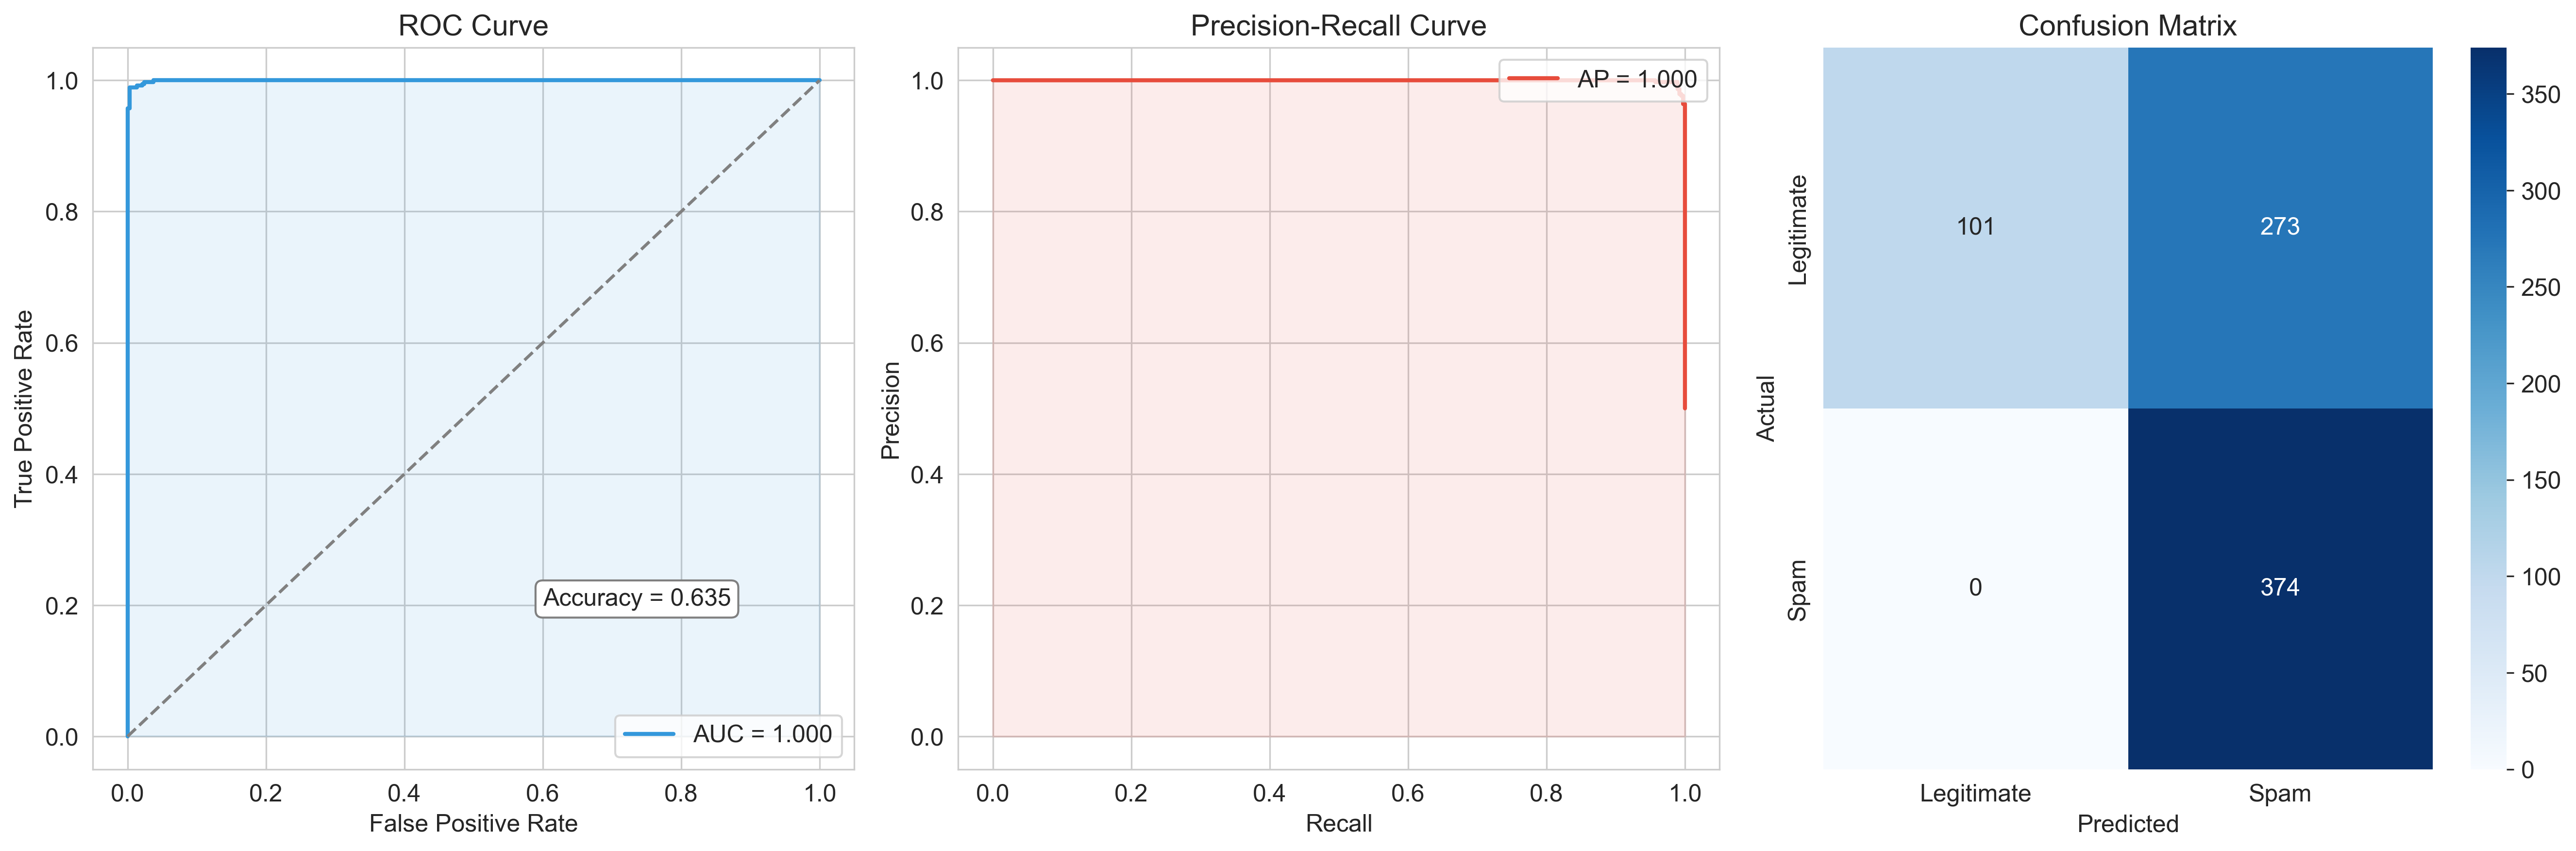
\includegraphics[width=0.8\textwidth]{../analysis/sms/sms_traditional_model_performance.png}
%     \caption{ROC Curve, Precision-Recall Curve, and Confusion Matrix for SMS Tradtional Model, trained using both UCI SMS Spam Collection Dataset [2] and SMS Spam Dataset [4]}
%     \label{fig:roc_curve_6}
% \end{figure}

\begin{figure}[htbp]
    \centering
    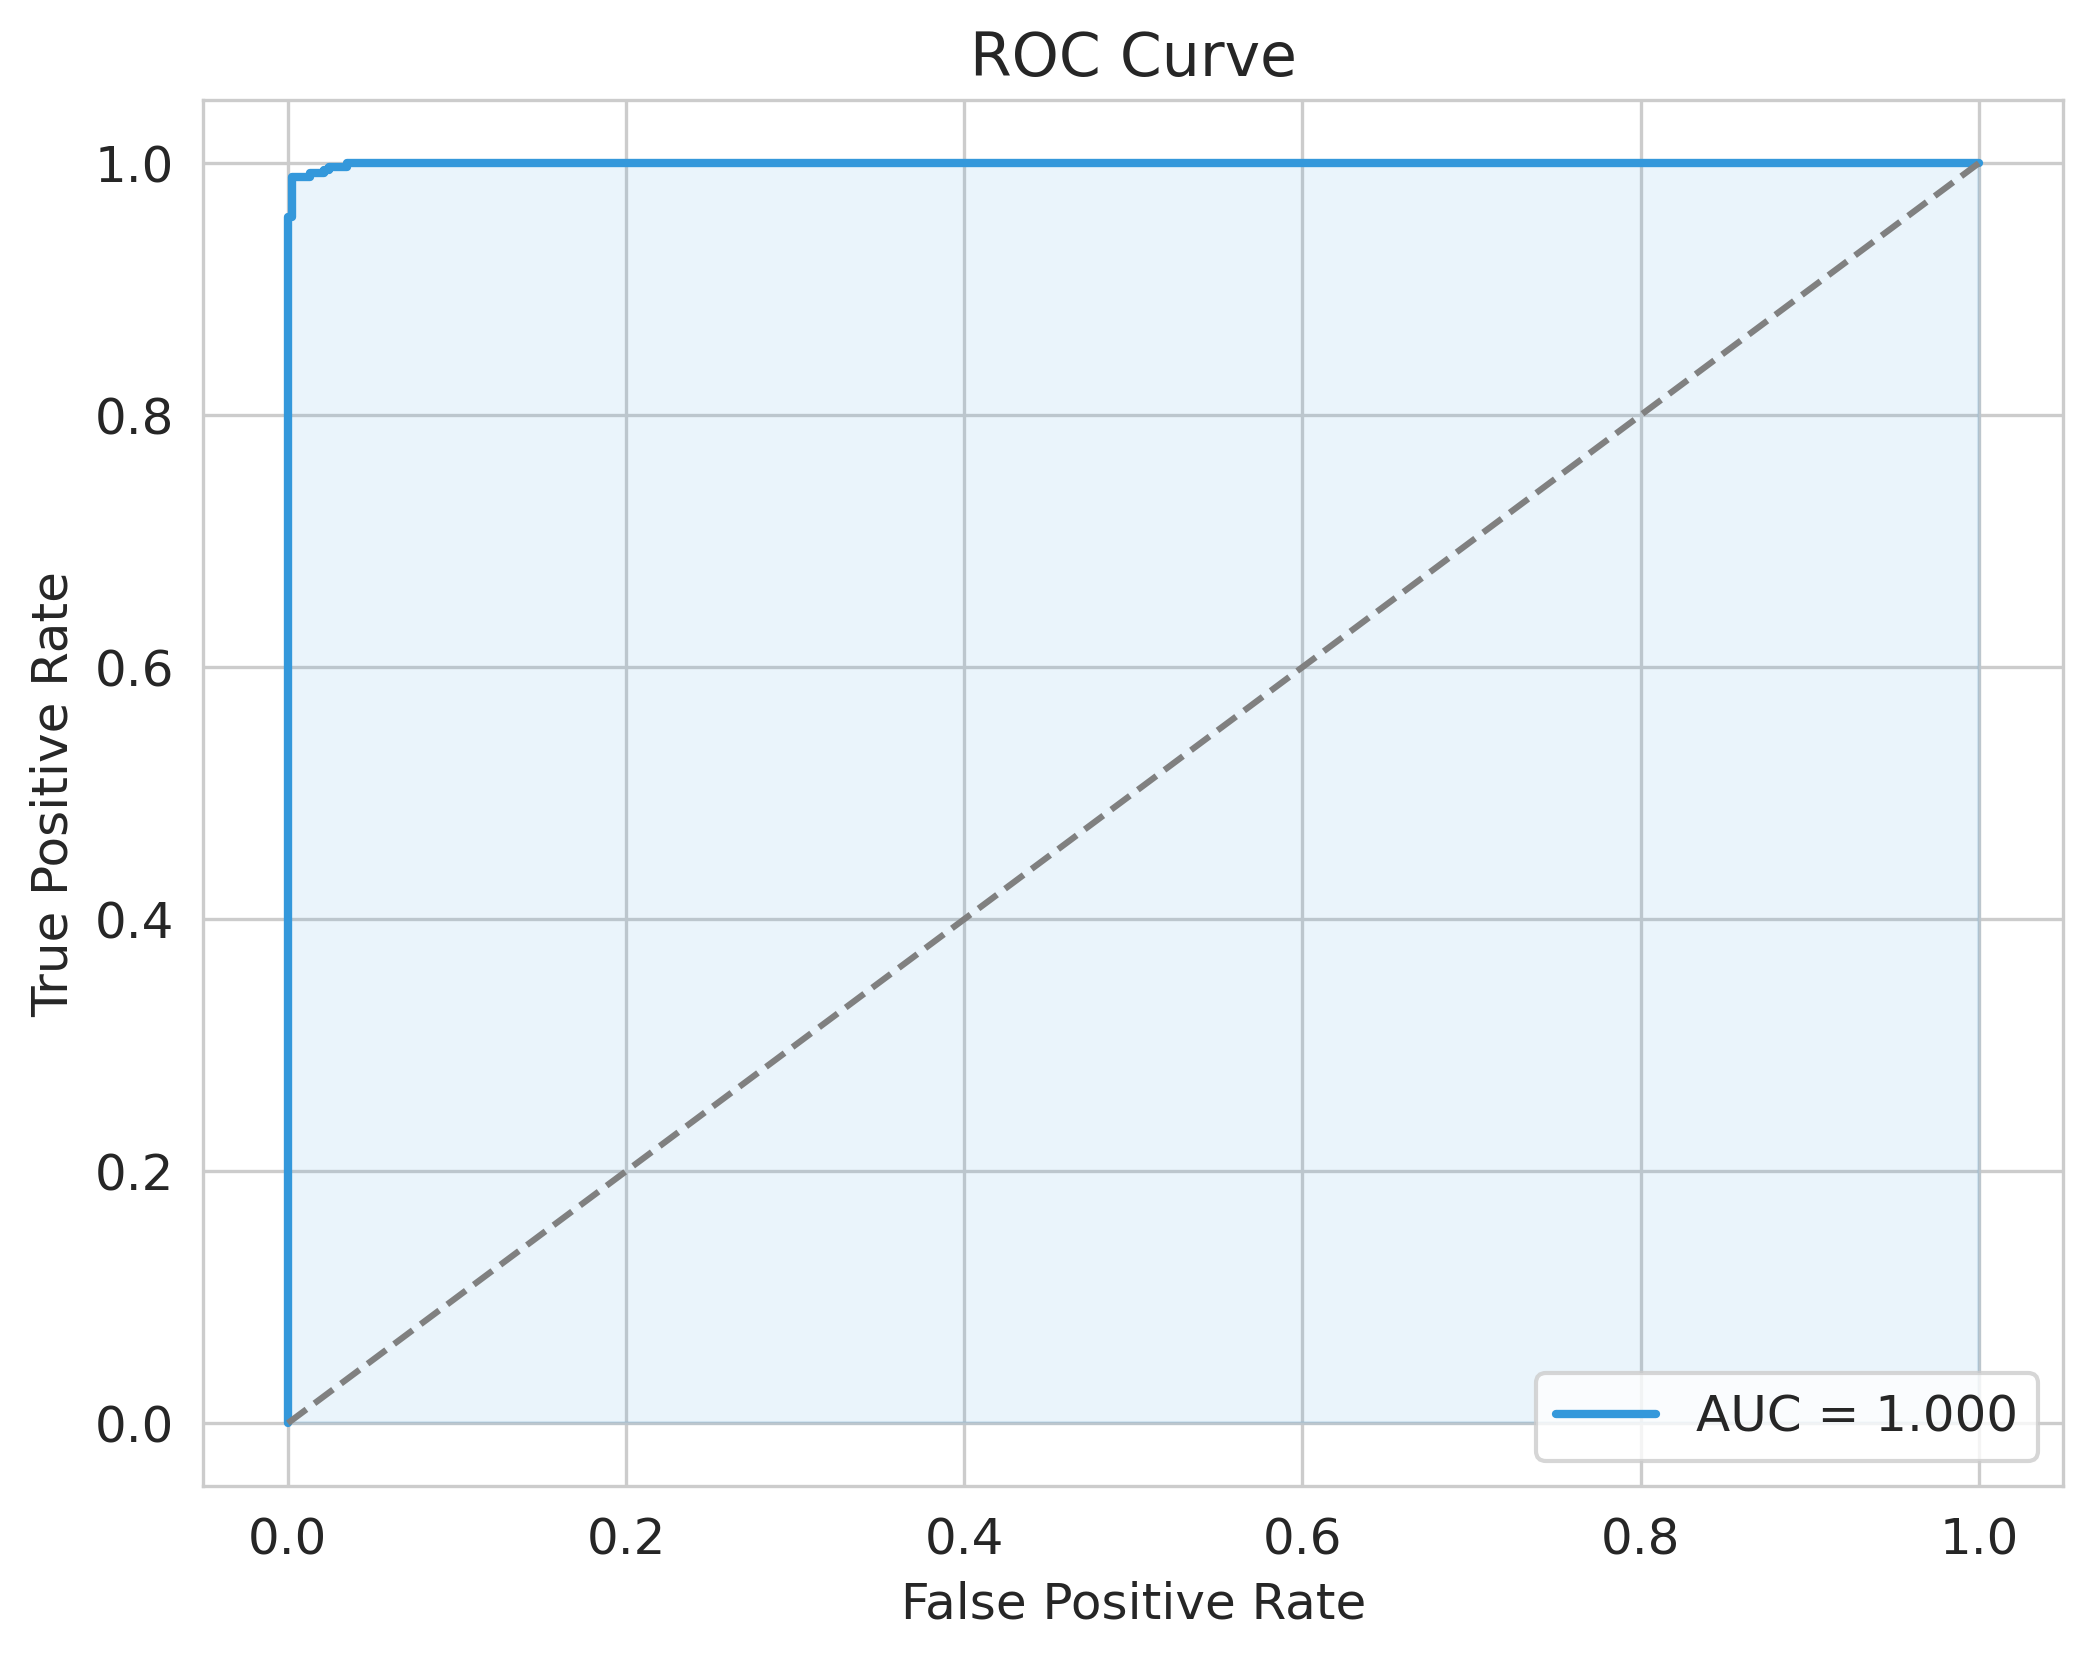
\includegraphics[width=0.8\textwidth]{../analysis/sms/traditional/roc_curve.png}
    \caption{ROC Curve for SMS Traditional Model, trained using both UCI SMS Spam Collection Dataset [2] and SMS Spam Dataset [4]}
    \label{fig:roc_curve_6}
\end{figure}

\begin{figure}[htbp]
    \centering
    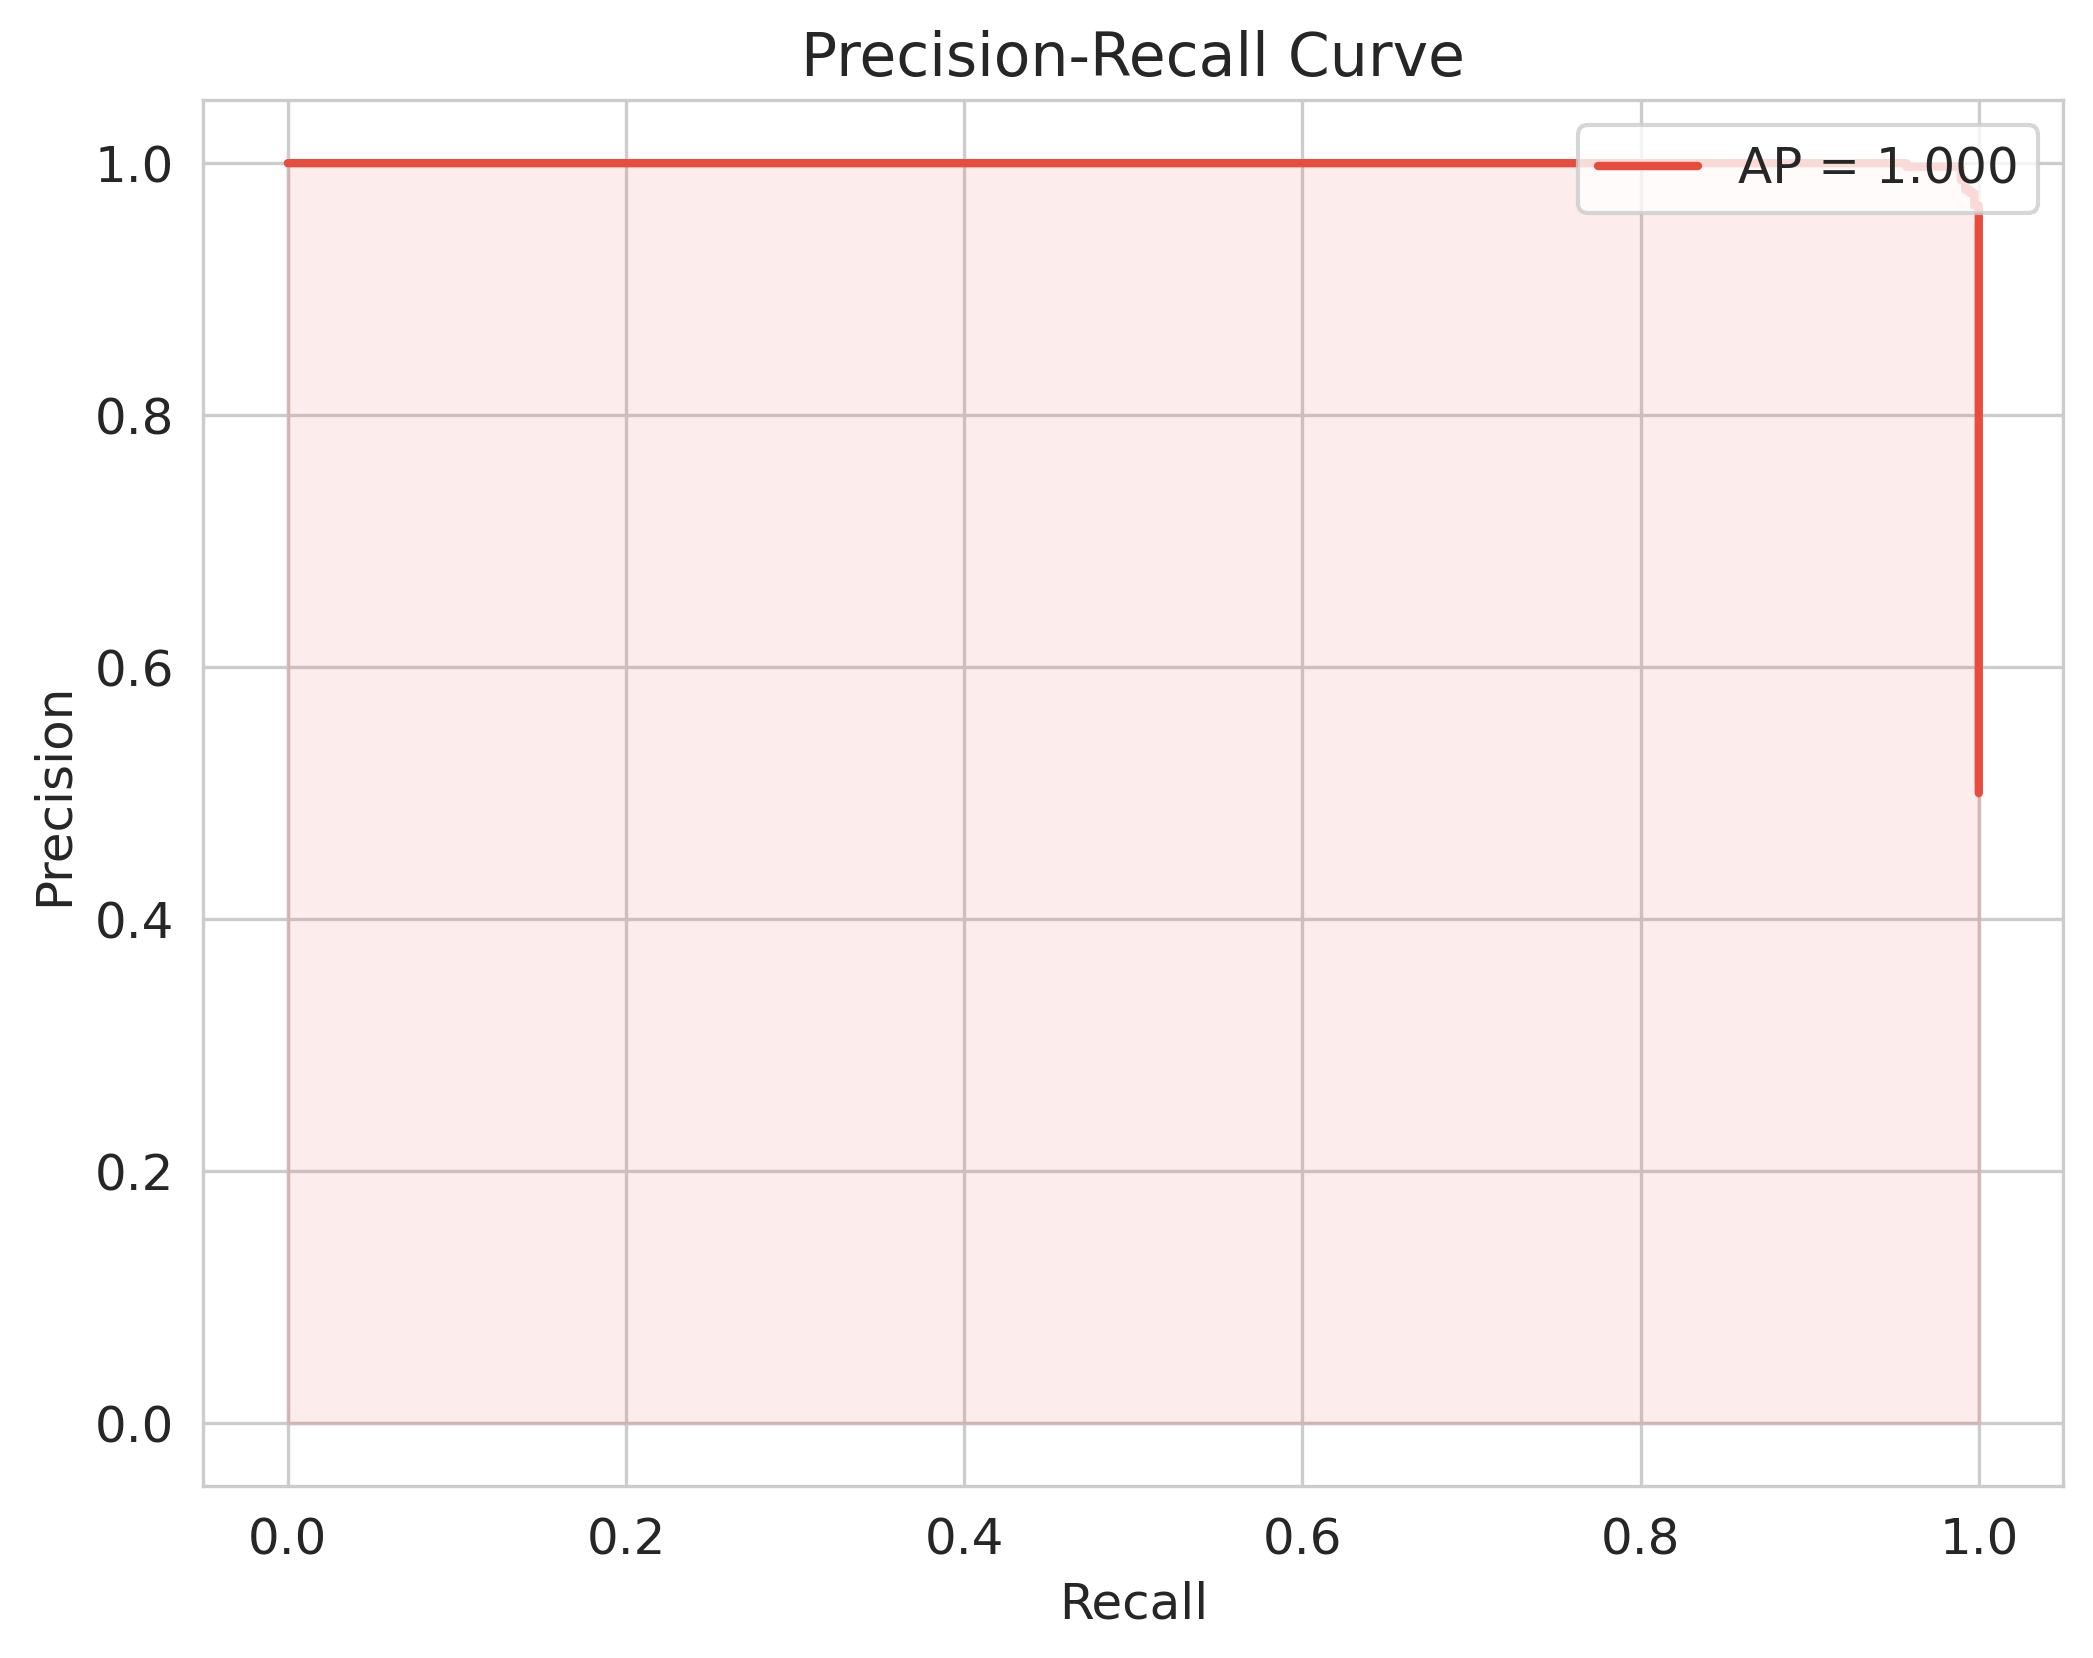
\includegraphics[width=0.8\textwidth]{../analysis/sms/traditional/precision_recall_curve.png}
    \caption{Precision-Recall Curve for SMS Traditional Model, trained using both UCI SMS Spam Collection Dataset [2] and SMS Spam Dataset [4]}
    \label{fig:precision_recall_curve_6}
\end{figure}

\begin{figure}[htbp]
    \centering
    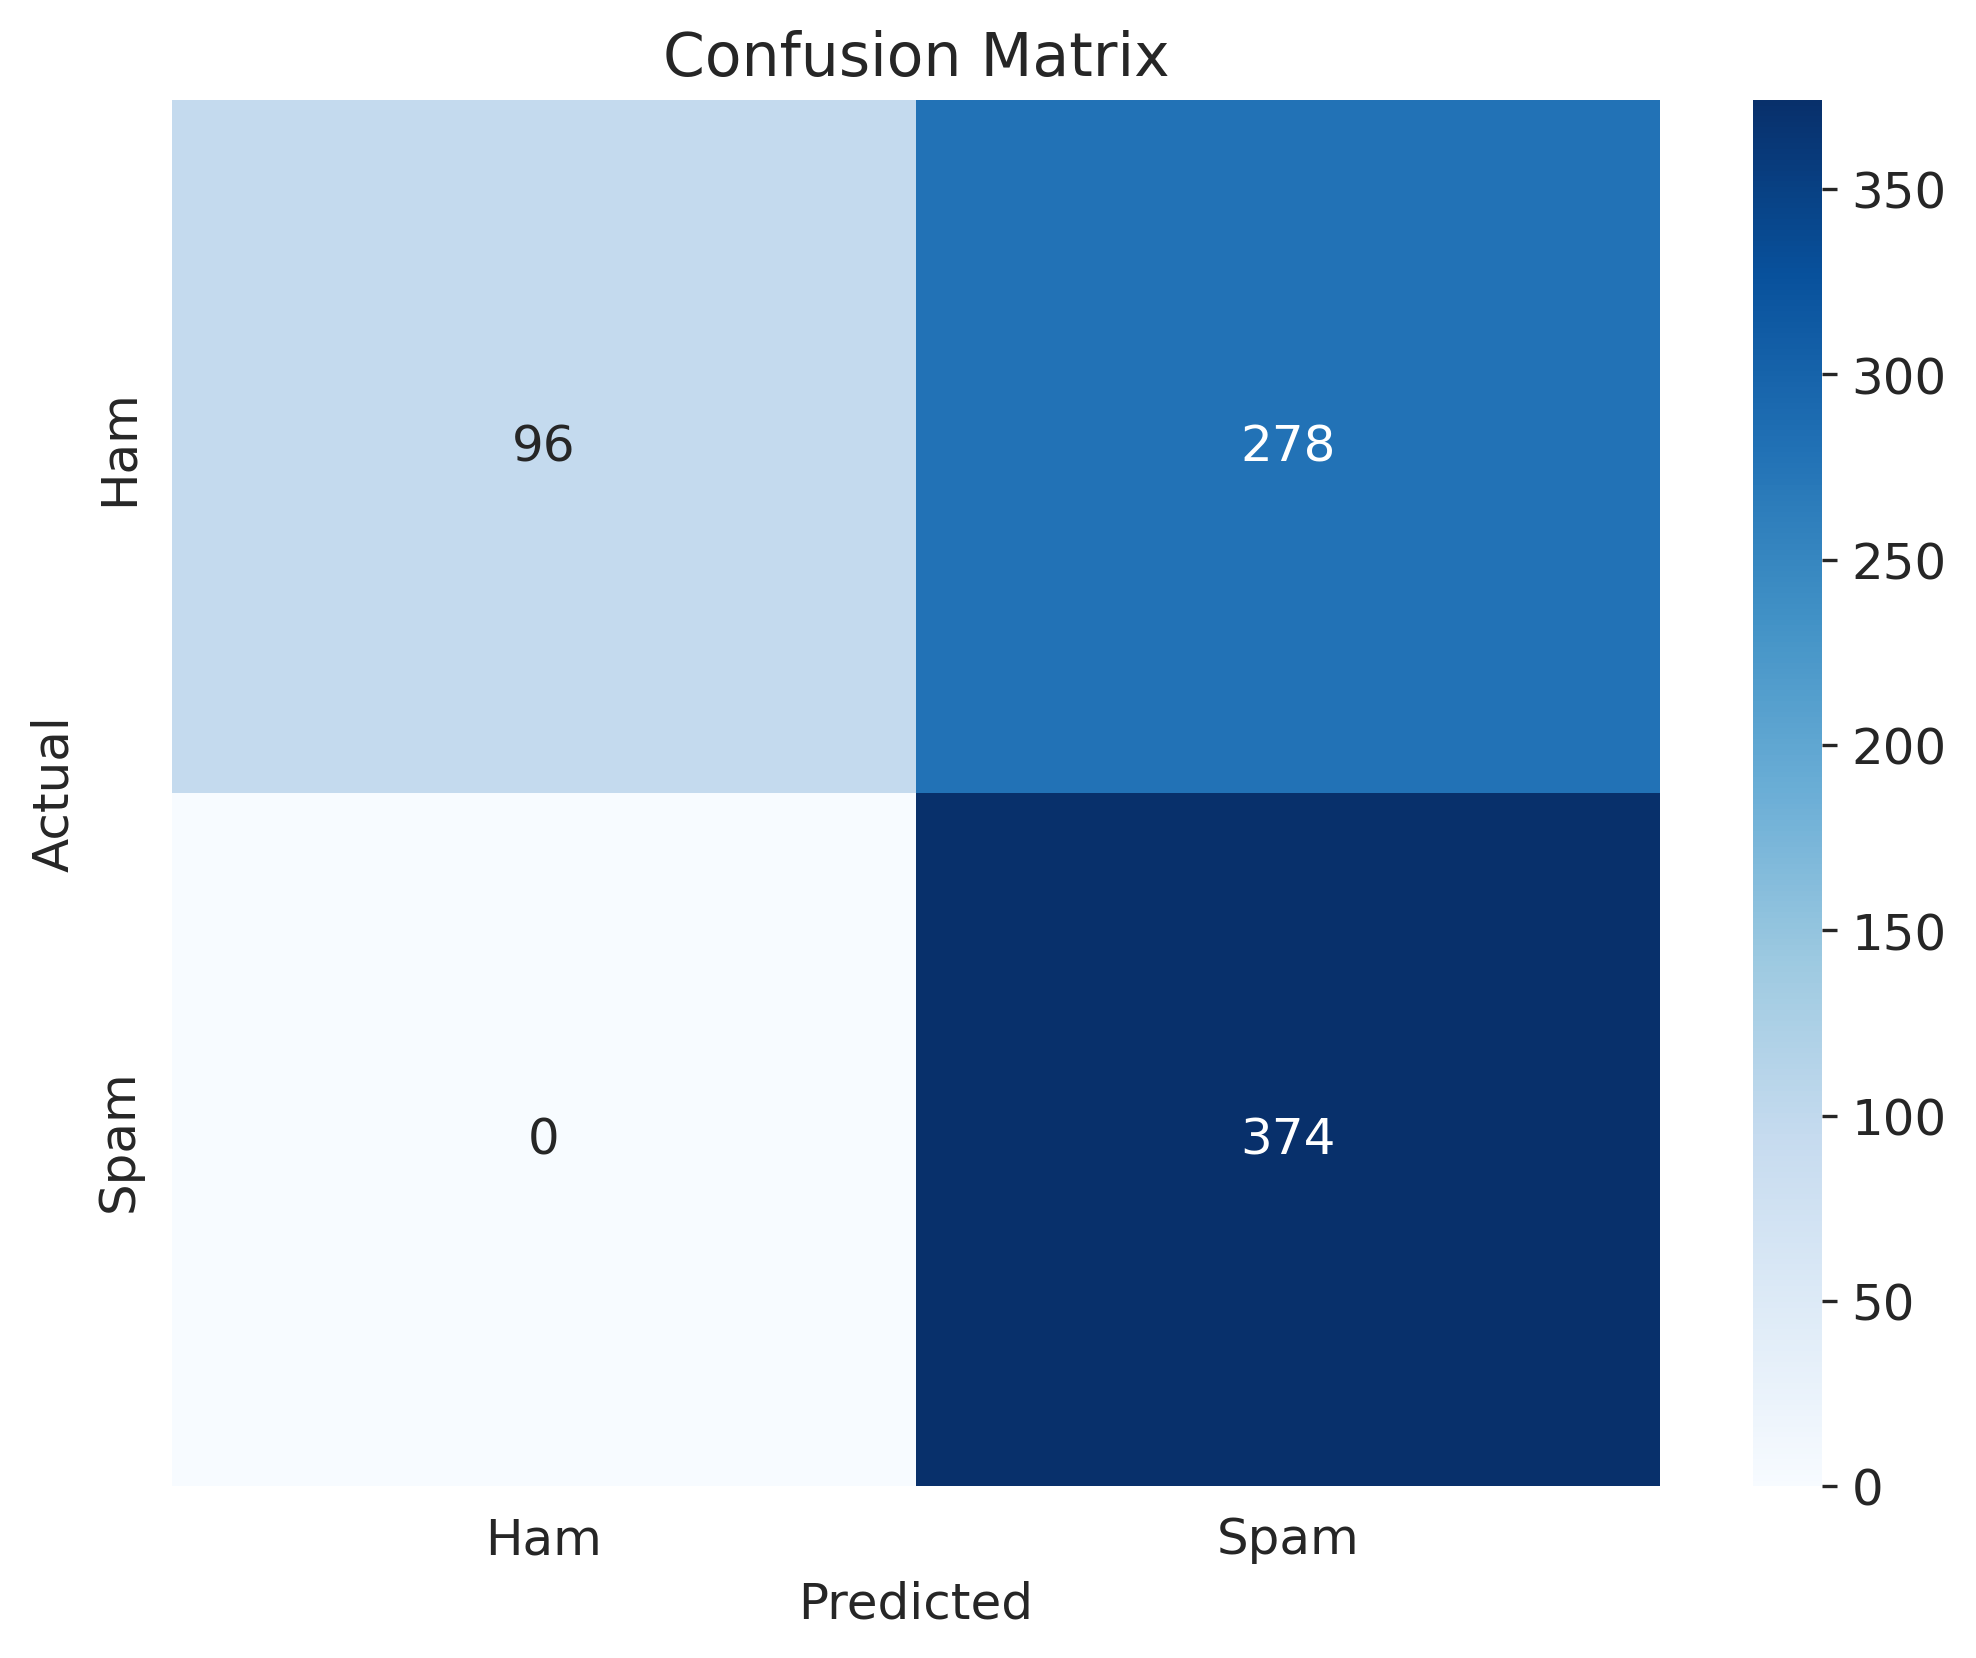
\includegraphics[width=0.8\textwidth]{../analysis/sms/traditional/confusion_matrix.png}
    \caption{Confusion Matrix for SMS Traditional Model, trained using both UCI SMS Spam Collection Dataset [2] and SMS Spam Dataset [4]}
    \label{fig:confusion_matrix_6}
\end{figure}

\begin{figure}[htbp]
    \centering
    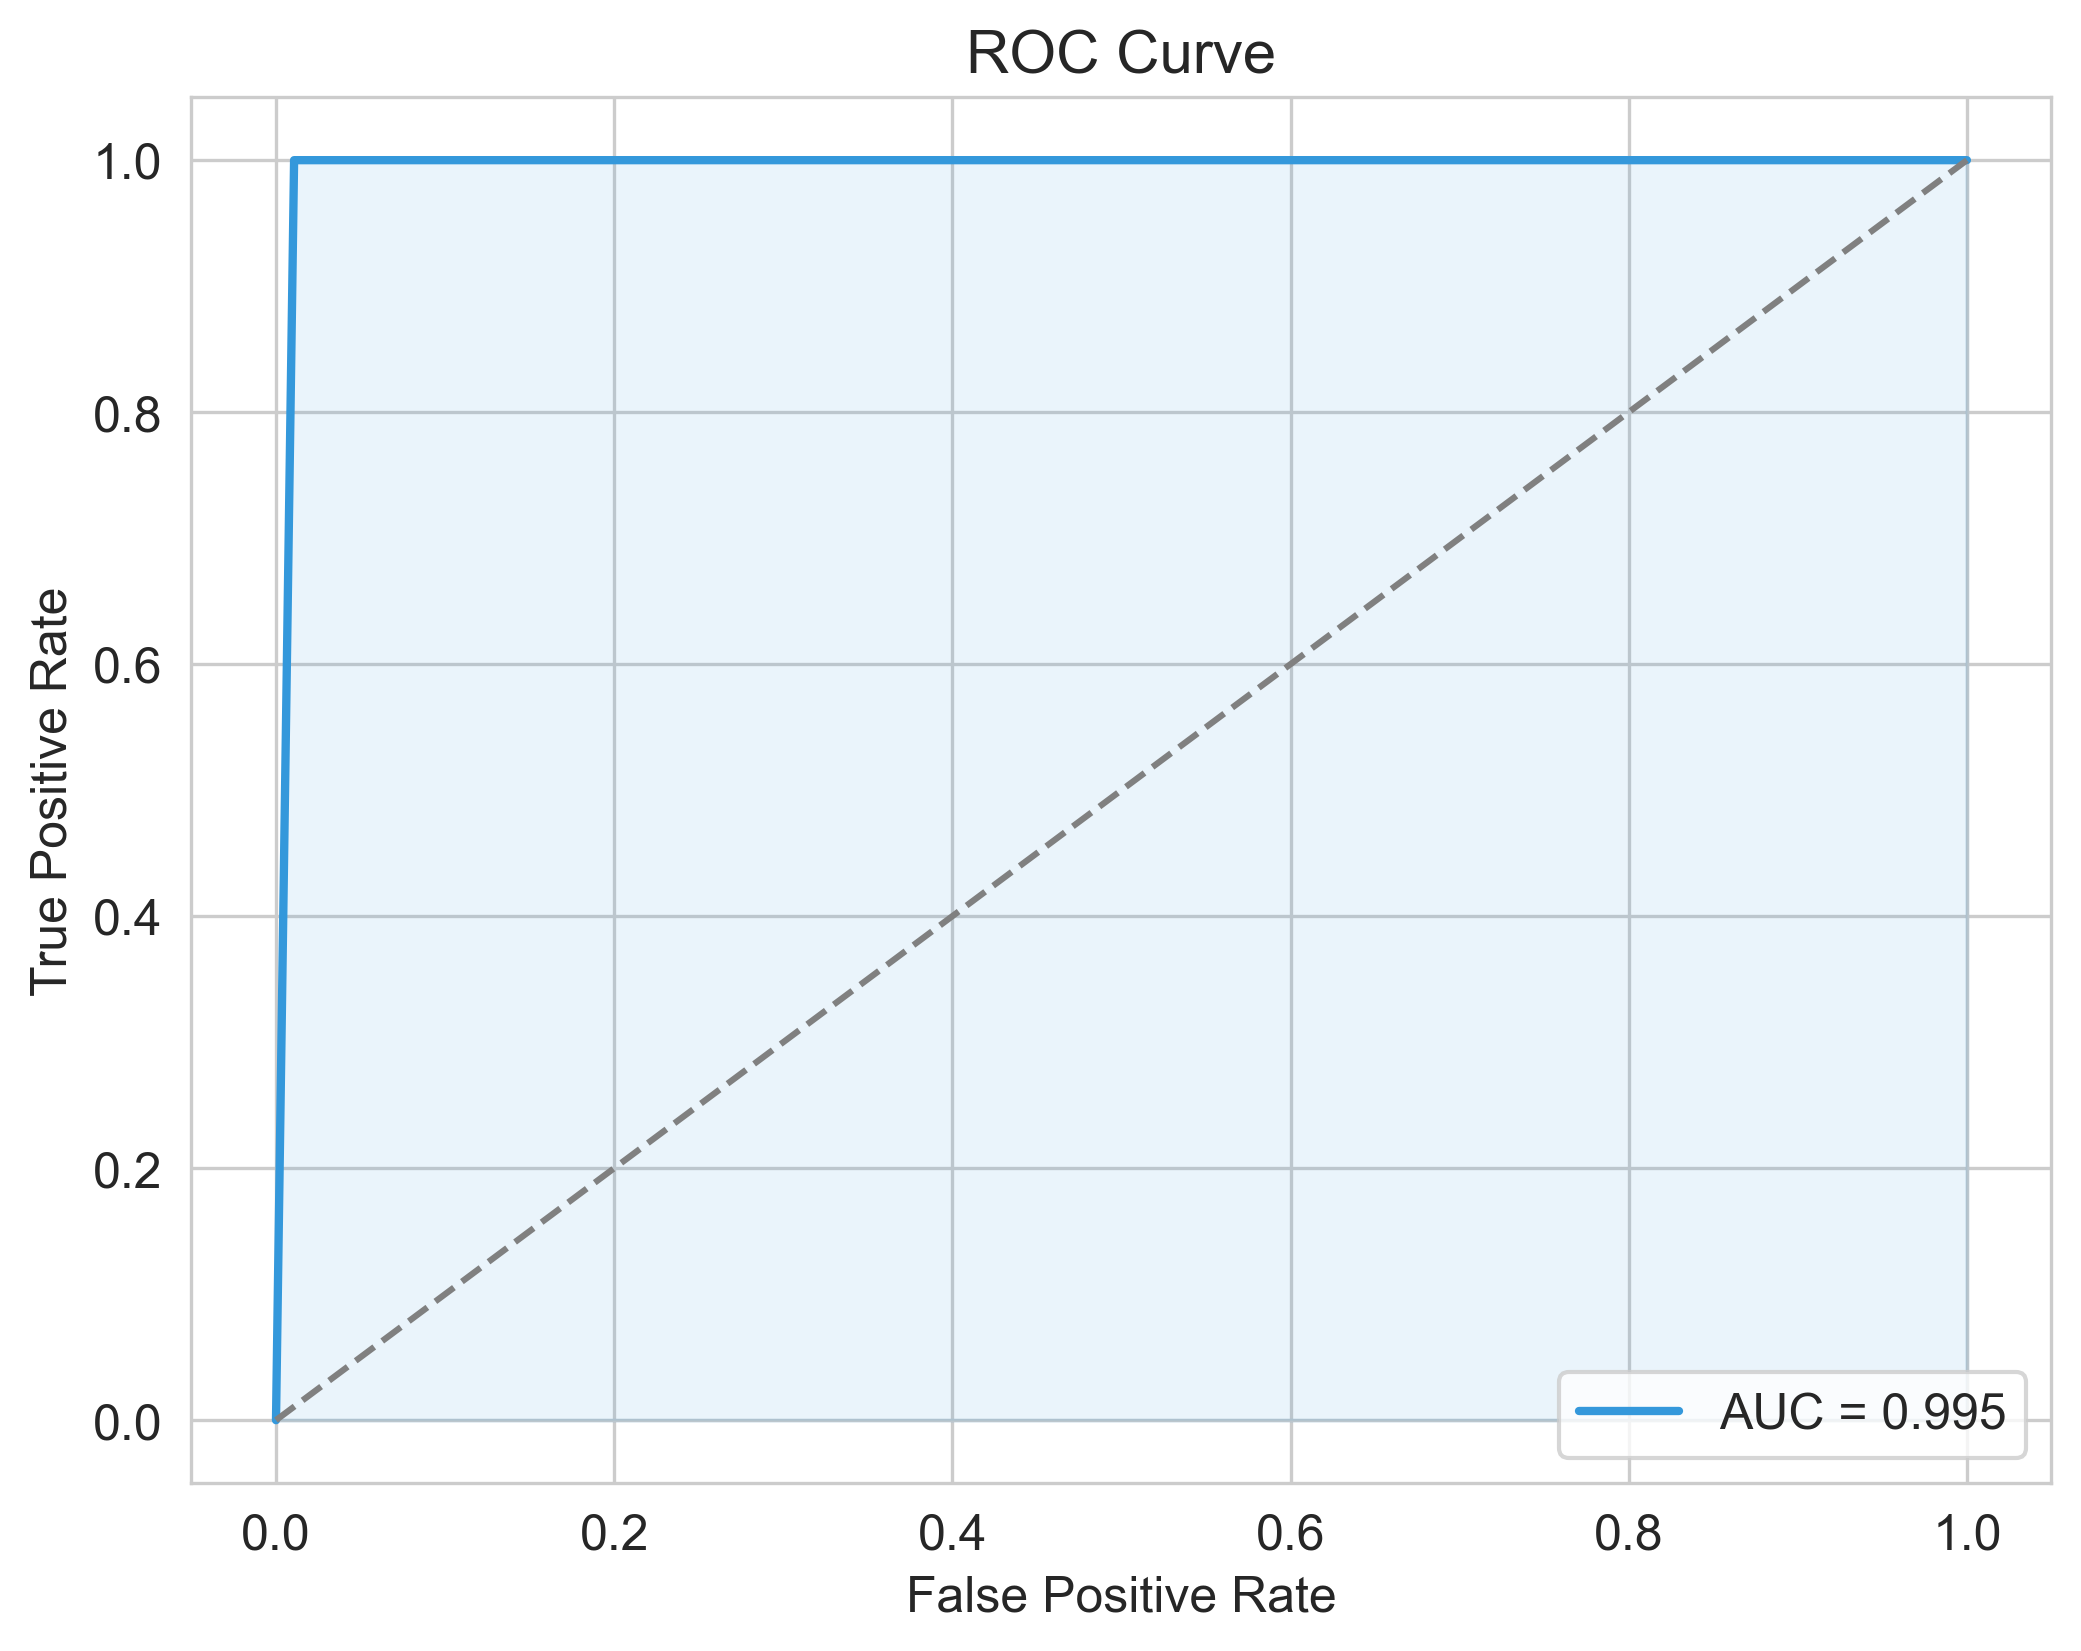
\includegraphics[width=0.8\textwidth]{../analysis/sms/hybrid/roc_curve.png}
    \caption{ROC Curve for SMS Hybrid Model, trained using both UCI SMS Spam Collection Dataset [2] and SMS Spam Dataset [4]}
    \label{fig:roc_curve_7}
\end{figure}

\begin{figure}[htbp]
    \centering
    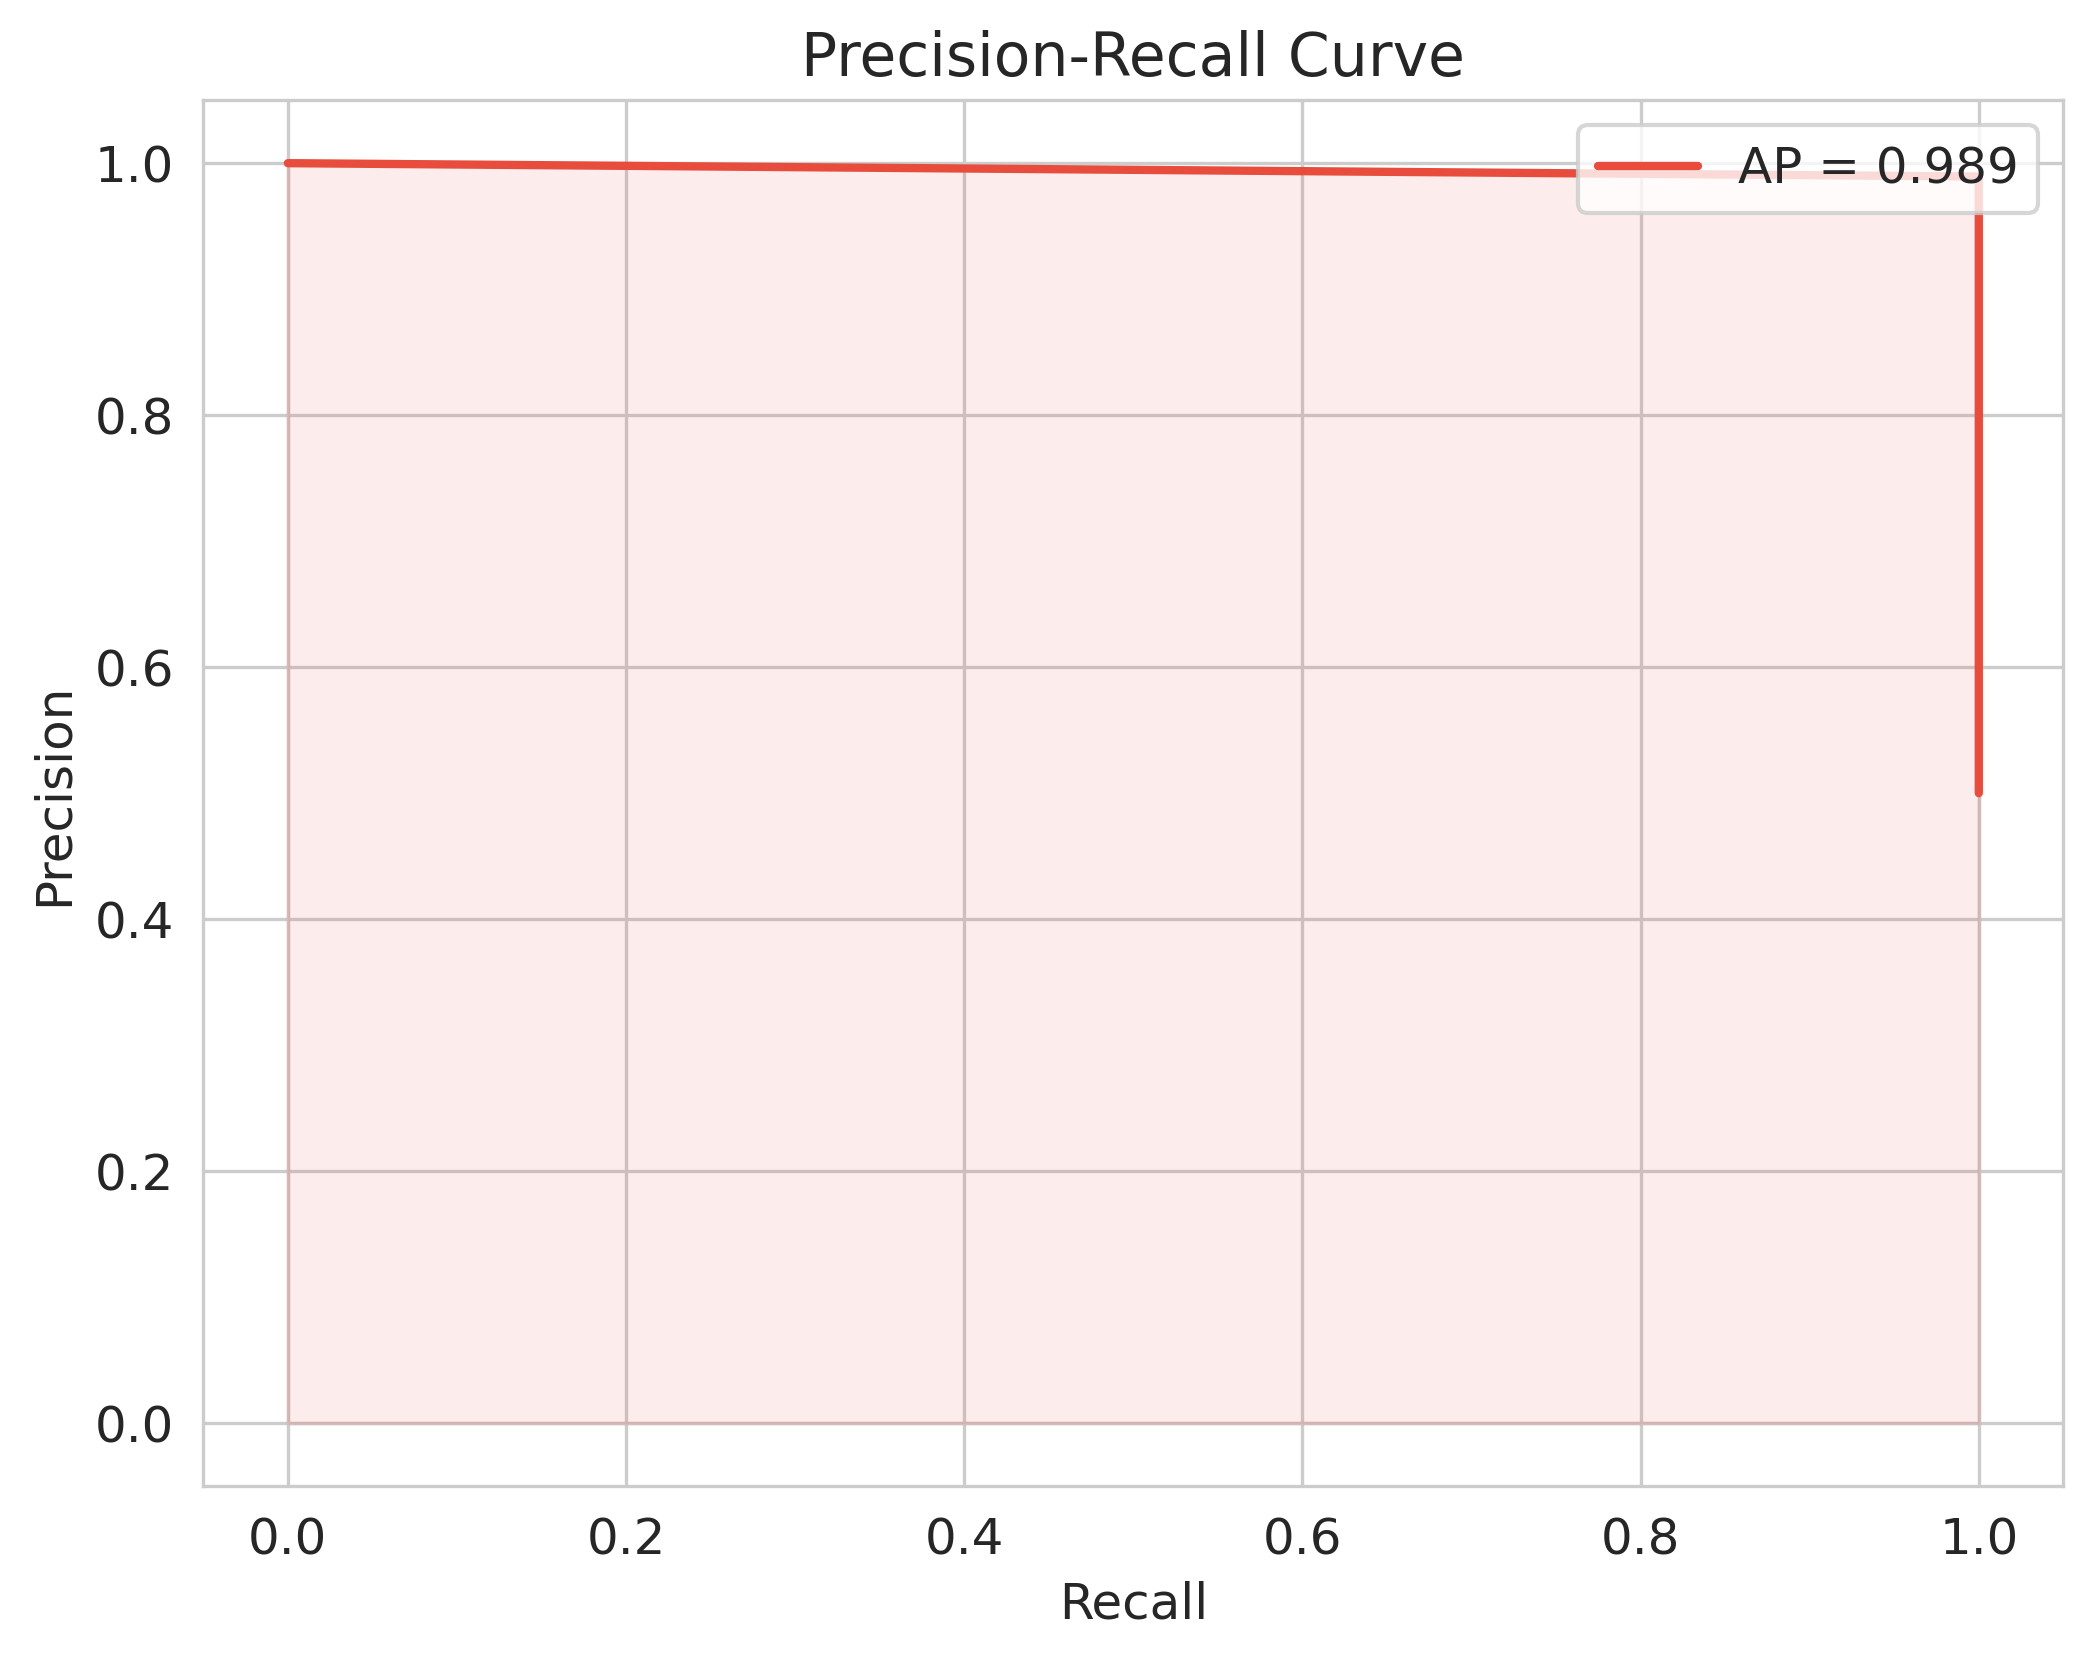
\includegraphics[width=0.8\textwidth]{../analysis/sms/hybrid/precision_recall_curve.png}
    \caption{Precision-Recall Curve for SMS Hybrid Model, trained using both UCI SMS Spam Collection Dataset [2] and SMS Spam Dataset [4]}
    \label{fig:precision_recall_curve_7}
\end{figure}

\begin{figure}[htbp]
    \centering
    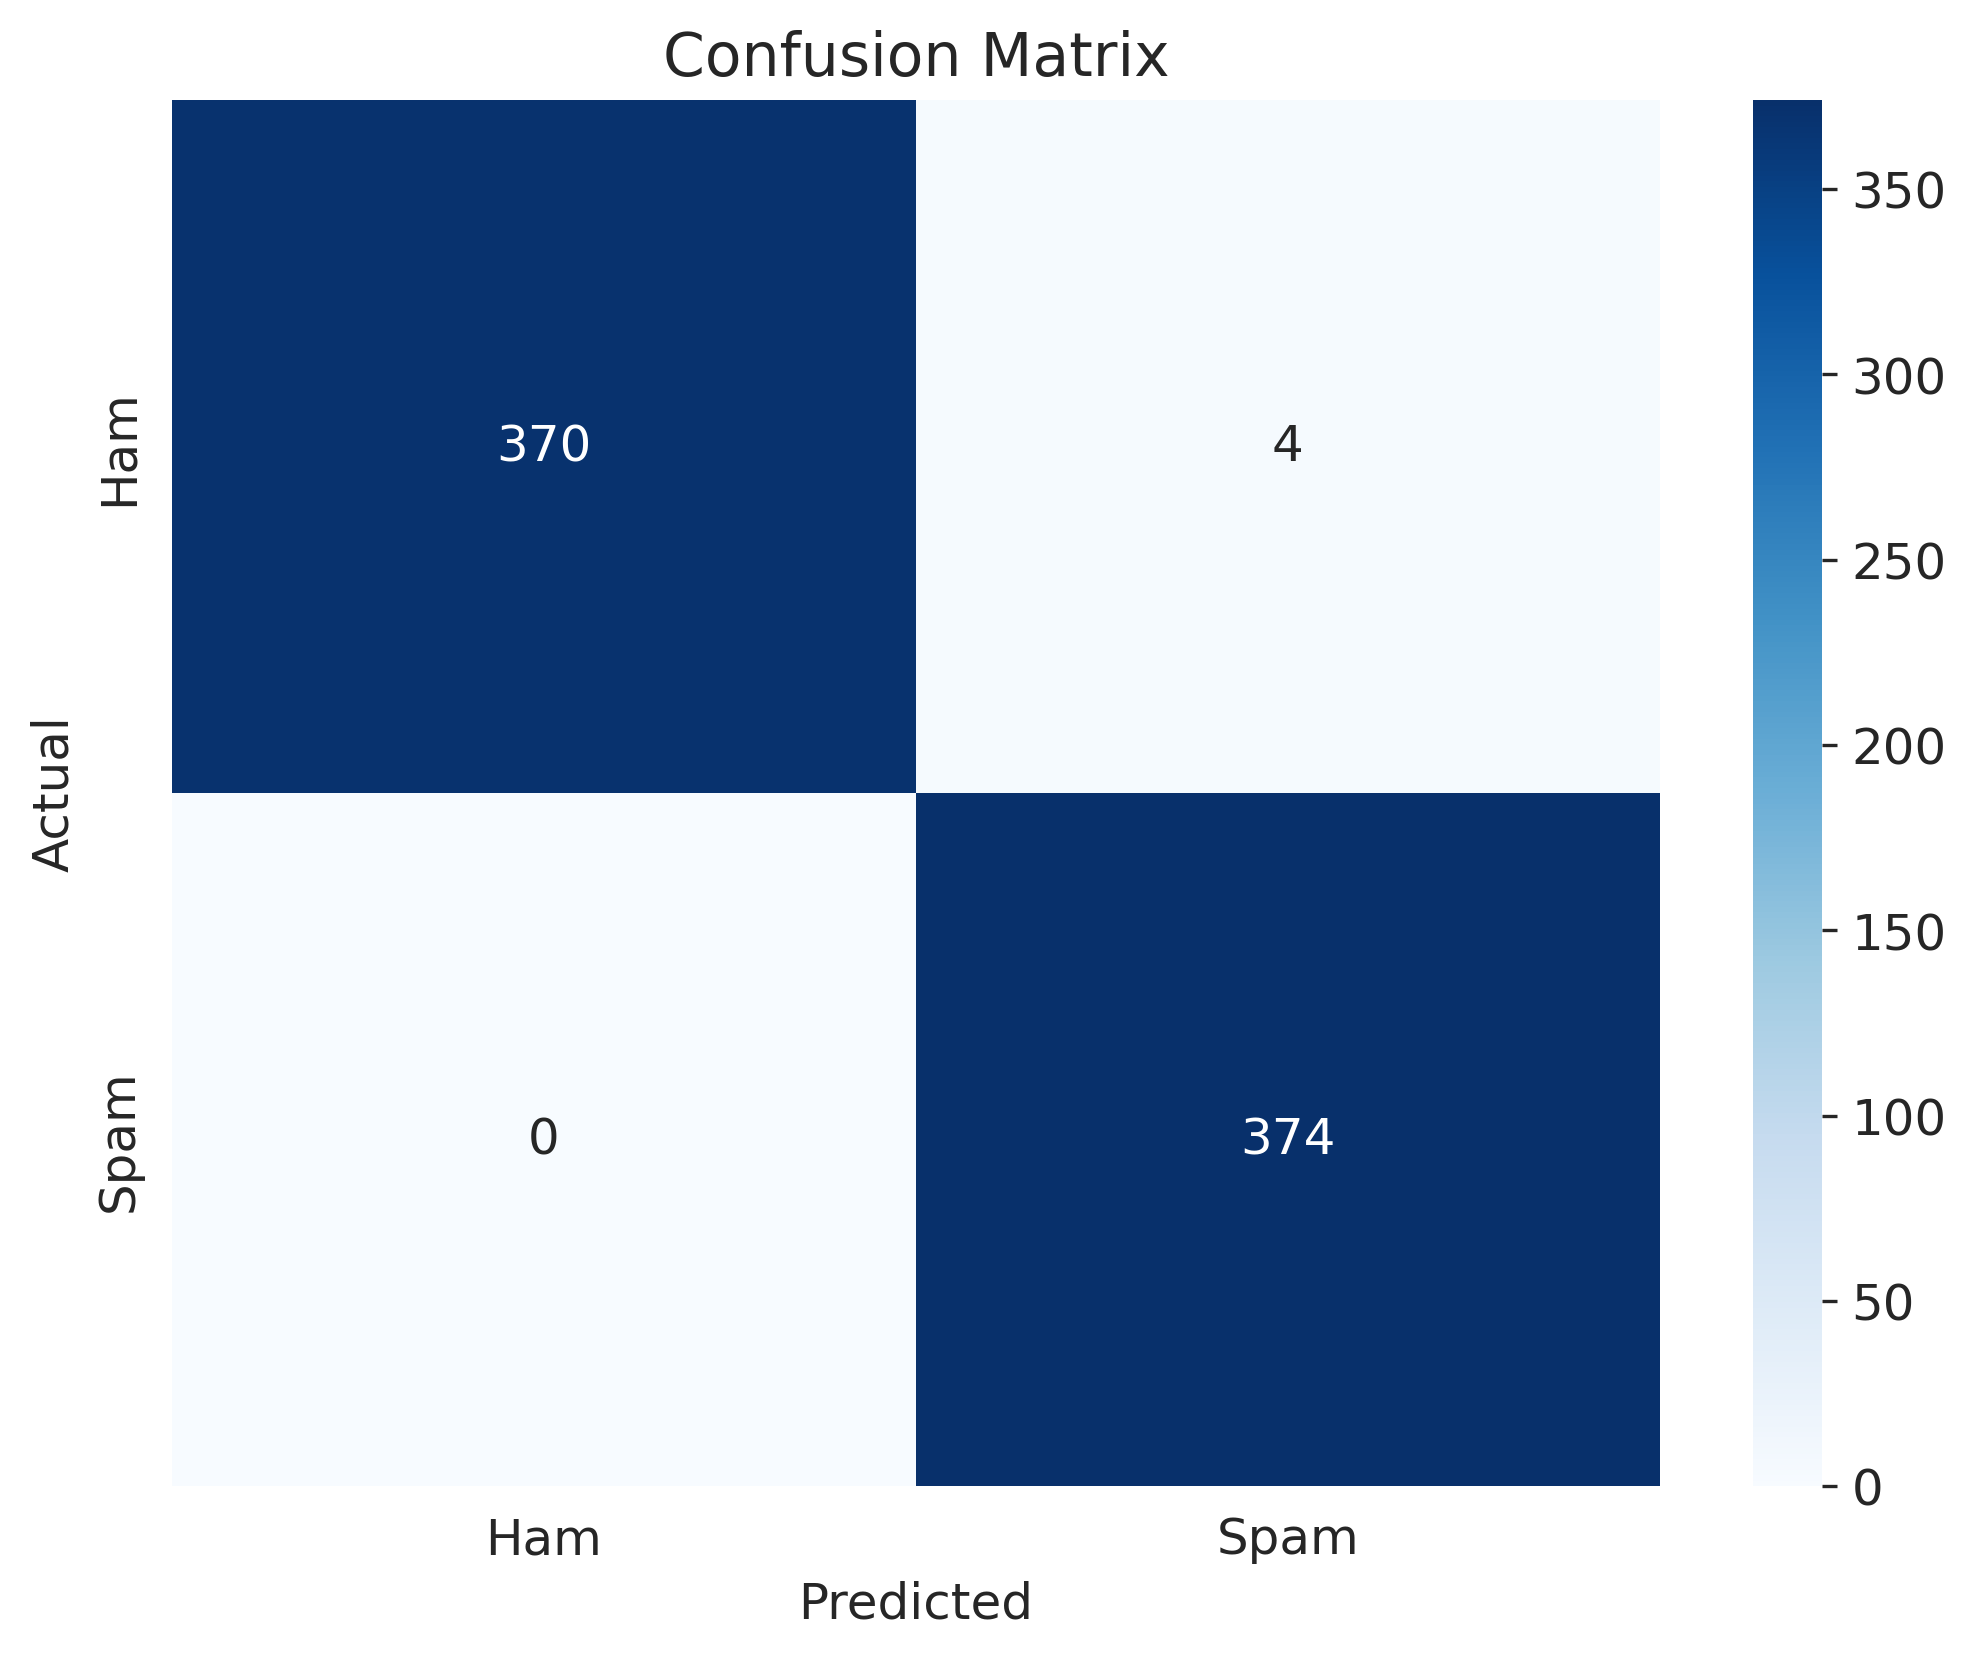
\includegraphics[width=0.8\textwidth]{../analysis/sms/hybrid/confusion_matrix.png}
    \caption{Confusion Matrix for SMS Hybrid Model, trained using both UCI SMS Spam Collection Dataset [2] and SMS Spam Dataset [4]}
    \label{fig:confusion_matrix_7}
\end{figure}

\newpage

\noindent
As shown in the tables above, we can see that the hybrid approach was able to achieve much better results than the traditional approach. The \textbf{hybrid approach} was able to achieve an \textbf{overall accuracy of 99\%}, while the \textbf{traditional approach} was only able to achieve an \textbf{accuracy of 63\%}. This shows that the hybrid approach is much more effective in detecting spam messages, especially when it comes to messages containing URLs. Furthermore, we can also see that the \textbf{hybrid approach} was able to achieve a much better \textbf{F1-Score}, with a score of \textbf{0.99}, while the \textbf{traditional approach} only achieved a score of \textbf{0.57}.

\subsection{Model Explainability and Interpretability}

\noindent
Understanding the decision-making process of spam-detection models is vital for building trust and transparency. While single metrics, such as classification accuracy provides useful performance metrics, it alone is an incomplete description of most real-world tasks [22]. Therefore, we must question why the model makes each decision. Studies regarding spam detectors have shown that the lack of interpretability in deep learning models can negatively impact model improvement efforts, "Interpretability remains a significant concern, as the complexity of these models often makes it challenging to understand the rationale behind specific classifications” [23]. Various techniques such as feature-importance scores can be used to help better understand which features are most important for the model's decision-making process. 

\begin{figure}[htbp]
    \centering
    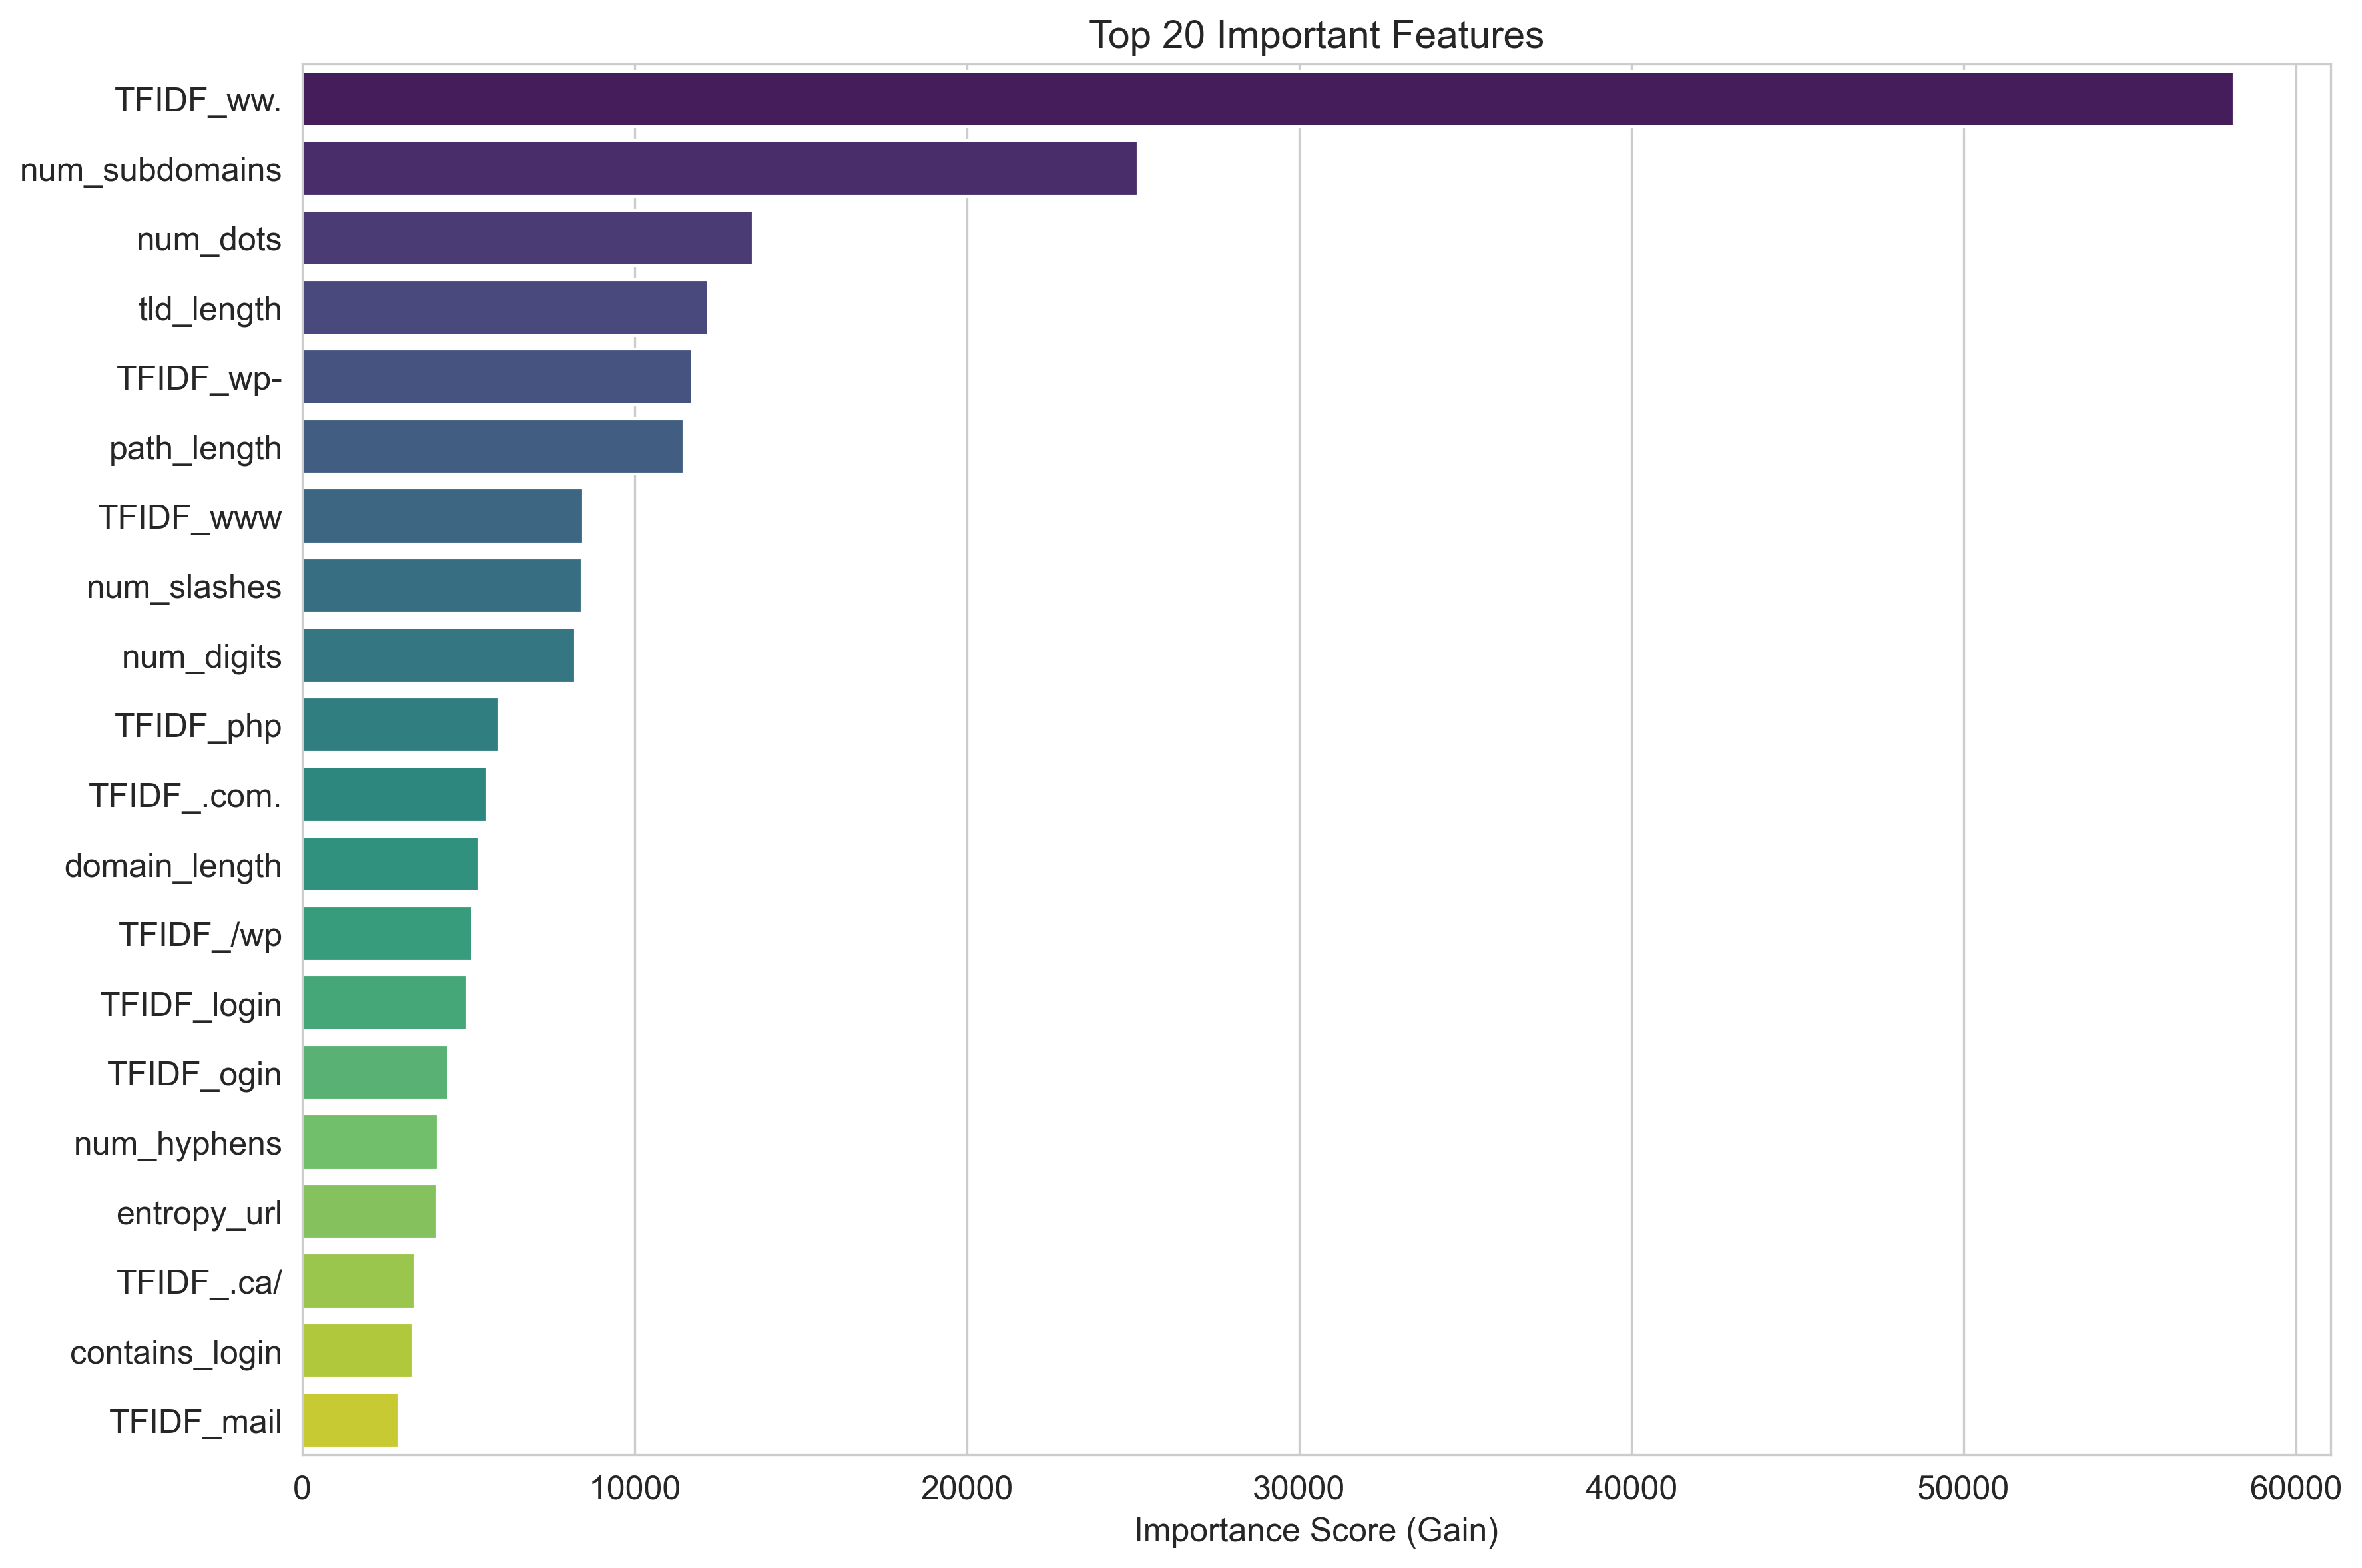
\includegraphics[width=0.8\textwidth]{../analysis/url/feature_importance.png}
    \caption{Feature Importance for URL Model}
    \label{fig:feature_importance_1}
\end{figure}

\noindent
To analyze which features were most important for out URL model, we plotted the top 20 predictors using gain-based feature importance. As shown in Figure~\ref{fig:feature_importance_1}, character-level TF-IDF n-grams such as \texttt{TFIDF\_ww.} and \texttt{TFIDF\_wp} dominate the TF-IDF features, while \texttt{num\_subdomains} and \texttt{num\_dots} lead among the engineered features. These results indicate the model's dependence on both structural URL characteristics and textual content. By analysing the feature importance, we are able to confirm that the model prioritizes meaningful features, giving us confidence in its decision-making process.

\subsection{LSTM Benchmark}

\noindent
To provide a deep learning baseline, using the Python TensorFlow library, we trained a bidirectional LSTM model on the SMS UCI dataset, using 5-fold Stratified Cross-Validation. The LSTM achieved the following results after training \textbf{1494 rows}, taking \textbf{12 secs}:

\begin{itemize}
    \item Accuracy: \textbf{95.65\%}
    \item AUC: \textbf{98.82\%}
    \item Average Precision: \textbf{98.92\%}
\end{itemize}

\begin{table}[htbp]
    \centering
    \caption{\textbf{SMS LSTM Model Classification Report}}
    \begin{tabular}{l c c c c}
    \toprule
     & \textbf{Precision} & \textbf{Recall} & \textbf{F1-Score} & Support \\
    \midrule
    \textbf{Legitimate} & \textbf{0.95} & \textbf{0.96} & \textbf{0.96} & 747 \\
    \textbf{Spam} & \textbf{0.96} & \textbf{0.95} & \textbf{0.96} & 747 \\
    \midrule
    \textbf{Accuracy} & & & \textbf{0.96} & 1494 \\
    Macro Avg & 0.96 & 0.96 & 0.96 & 1494 \\
    Weighted Avg & 0.96 & 0.96 & 0.96 & 1494 \\
    \bottomrule
    \end{tabular}
    \label{tab:classification_report_6}
\end{table}

\noindent
While the LSTM demonstrated strong performance, our Random Forest model slightly outperformed it with an accuracy of 97.00\%. This highlights that, for structured short-form text like SMS with limited data, traditional models with proper preprocessing can not only match but also exceed the performance of deep learning models. Perhaps if we had a much larger dataset, the LSTM model would have been able to outperform the Random Forest model. However, this is not the case here, as we are limited by the size of the dataset.

\subsection{Future Deployment Strategy}

\noindent
A functional web application has already been developed and deployed locally, allowing users to input messages, which then communicates with the backend API endpoints for real-time spam classification. Future deployment will incolve transitioning the application from localhost to a production enviornment. This will include containerizing the application using Docker and hosting it on a scalable cloud platform, such as AWS or Heroku. Kubernetes will be used to manage the containerized application for scalability and reliability. Additionally, to ensure our model remains effective over time, we will implement a monitoring system such as Grafana, to track performance and trigger updates. This pipeline ensures the application remains scalable and responsive to real-world usage.

\subsection*{Conclusion}
In conclusion, our study demonstrates the effectiveness of a hybrid approach for spam detection by combining traditional text-based models with a dedicated URL classification model. By addressing the limitations of existing datasets and employing advanced feature extraction techniques, we achieved high accuracy and robustness across SMS, email, and YouTube comments. The results indicate that our hybrid model significantly outperforms traditional methods, particularly in scenarios involving URLs. Additionally, training datasets being adequately balanced is an absolute must when it comes to reliable spam detection, as well as reliable training techniques such as Stratified K-fold. Overall, this research highlights the importance of continuous innovation in spam detection methodologies to adapt to evolving threats in digital communication.


\newpage
\subsection*{References}
[1] S. D. Gupta, S. Saha, and S. K. Das, "SMS Spam Detection Using Machine Learning," *J. Phys. Conf. Ser.*, vol. 1797, no. 1, p. 012017, Feb. 2021, doi: 10.1088/1742-6596/1797/1/012017.
\newline
\newline
[2] UCI Machine Learning Repository, "SMS Spam Collection Dataset," [Online]. Available: https://www.kaggle.com/datasets/uciml/sms-spam-collection-dataset. [Accessed: 2025-03-24].
\newline
\newline
[3] S. Kumar, "Malicious and Benign URLs," [Online]. Available: https://www.kaggle.com/datasets/siddharthkumar25/malicious-and-benign-urls/data. [Accessed: Mar. 24, 2025].
\newline
\newline
[4] T. Kumar, "SMS Spam Dataset," [Online]. Available: https://www.kaggle.com/datasets/tinu10kumar/sms-spam-dataset. [Accessed: Mar. 24, 2025].
\newline
\newline
[5] N. Bharathi, "Email Spam Dataset," [Online]. Available: https://www.kaggle.com/datasets/nitishabharathi/email-spam-dataset?select=enronSpamSubset.csv. [Accessed: Mar. 24, 2025].
\newline
\newline
[6] V. Venky, "Spam Mails Dataset," [Online]. Available: https://www.kaggle.com/datasets/venky73/spam-mails-dataset. [Accessed: Mar. 24, 2025].
\newline
\newline
[7] A. Waheed, "Youtube Comments Spam Dataset," [Online]. Available: https://www.kaggle.com/datasets/ahsenwaheed/youtube-comments-spam-dataset. [Accessed: Mar. 24, 2025].
\newline
\newline
[8] S. Gawai and S. S. Salunke, "Classifying SMS as Spam or Ham Leveraging NLP and Machine Learning Techniques," in *2024 International Conference on Communication, Computing and Internet of Things (IC3IoT)*, 2024, pp. 1-6.
\newline
\newline
[9] M. F. Johari, K. L. Chiew, A. R. Hosen, and A. S. Khan, “Key insights into recommended SMS spam detection datasets,” Scientific Reports, vol. 15, Art. 8162, 2025.
\newline
\newline
[10] H. Al-Kaabi, A. D. Darroudi, and A. K. Jasim, “Survey of SMS Spam Detection Techniques: A Taxonomy,” AlKadhim Journal for Computer Science, vol. 2, no. 4, pp. 23–34, Dec. 2024.
\newline
\newline
[11] Y. Bilgen and M. Kaya, “EGMA: Ensemble learning-based hybrid model approach for spam detection,” Applied Sciences, vol. 14, no. 21, Art. 9669, 2024.
\newline
\newline
[12] H. C. Altunay, “SMS spam detection system based on deep learning architectures for Turkish and English messages,” Applied Sciences, vol. 14, no. 24, Art. 11804, 2024.
\newline
\newline
[13] M. A. Shaaban, Y. F. Hassan, and S. K. Guirguis, “Deep convolutional forest: A dynamic deep ensemble approach for spam detection in text,” Evol. Intell., vol. 8, no. 6, pp. 4897–4909, 2022.
\newline
\newline
[14] E. H. Tusher, M. A. Ismail, M. A. Rahman, A. H. Alenezi, and M. Uddin, “Email Spam: A comprehensive review of optimized detection methods, challenges, and open research problems,” IEEE Access, vol. 12, pp. 143627–143657, 2024.
\newline
\newline
[15] X. Liu, “Deciphering spam through AI: From traditional methods to deep learning advancements in email security,” in Proc. Int. Conf. on Eng. Management, IT \& Intelligence (EMITI), 2024, pp. 54–60.
\newline
\newline
[16] G. Airlangga, “Spam Detection on YouTube Comments Using Advanced Machine Learning Models: A Comparative Study,” Brilliance: Research of Artificial Intelligence, vol. 4, no. 2, pp. 500–508, 2024.
\newline
\newline
[17] M. Sam’an and K. Imaddudin, “Hybrid deep learning model for YouTube spam comment detection,” Int. J. Electr. Comput. Eng., vol. 14, no. 3, pp. 3313–3319, 2024.
\newline
\newline
[18] H. Oh, “A YouTube spam comments detection scheme using cascaded ensemble machine learning model,” IEEE Access, vol. 9, pp. 144121–144128, 2021.
\newline
\newline
[19] M. R. Al Saidat, S. Y. Yerima, and K. Shaalan, “Advancements of SMS spam detection: A comprehensive survey of NLP and ML techniques,” Procedia Comput. Sci., vol. 244, pp. 248–259, 2024.
\newline
\newline
[20] A. S. Xiao and Q. Liang, “Spam detection for YouTube video comments using machine learning approaches,” Machine Learning with Applications, vol. 16, Art. 100550, 2024.
\newline
\newline
[21] N. R. R. Rao and G. A. F. Vinodhini, “Measuring the efficiency of random forest, naive bayes, multilayer perceptron and support vector machine in email spam detection,” in Proc. ICONNECT-2024, 2025.
\newline
\newline
[22] F. Doshi-Velez and B. Kim, "Towards a Rigorous Science of Interpretable Machine Learning," arXiv Preprint arXiv:1702.08608, Feb. 2017. [Online]. Available: https://arxiv.org/abs/1702.08608
\newline
\newline
[23] X. Liu, “Deciphering Spam Through AI: From Traditional Methods to Deep Learning Advancements in Email Security,” Proceedings of the 1st International Conference on Engineering Management, Information Technology and Intelligence, pp. 553–558, 2024, doi: https://doi.org/10.5220/0012958700004508.


\newpage

\end{document}